\documentclass[letterpaper]{article}


\usepackage[final,nonatbib]{neurips_2021}




\usepackage[utf8]{inputenc} %
\usepackage[T1]{fontenc}    %
\usepackage{hyperref}       %
\usepackage{url}            %
\usepackage{booktabs}       %
\usepackage{amsfonts}       %
\usepackage{nicefrac}       %
\usepackage{microtype}      %
\usepackage{xcolor}         %
\usepackage{graphicx}
\usepackage{subcaption}
\usepackage{booktabs} %
\usepackage{lipsum}
\usepackage{amsmath}
\usepackage{amssymb, amsthm, latexsym}
\usepackage{multirow}
\usepackage{wrapfig}


\usepackage{algorithm,algorithmic}



\usepackage{enumitem}
\usepackage{caption}
\setlist[itemize]{itemsep=0pt}


\newcommand{\Exp}{\mathbf{E}}
\newcommand{\Prob}{\mathbf{P}}
\newcommand{\R}{\mathbb{R}}
\newcommand{\eqdef}{\stackrel{\text{def}}{=}}
\newcommand{\ve}[2]{\left\langle #1 , #2 \right\rangle}
\def\<#1,#2>{\left\langle #1,#2\right\rangle}

\usepackage{thmtools}

\newtheorem{lemma}{Lemma}[section]
\newtheorem{theorem}{Theorem}[section]
\newtheorem{definition}{Definition}[section]
\newtheorem{proposition}{Proposition}[section]
\newtheorem{assumption}{Assumption}[section]
\newtheorem{corollary}{Corollary}[section]
\newtheorem{remark}{Remark}[section]





\newcommand\tagthis{\addtocounter{equation}{1}\tag{\theequation}}
\newcommand{\argmin}{\mathop{\arg\!\min}}

\newcommand{\cA}{{\cal A}}
\newcommand{\cB}{{\cal B}}
\newcommand{\cC}{{\cal C}}
\newcommand{\cD}{{\cal D}}
\newcommand{\cE}{{\cal E}}
\newcommand{\cF}{{\cal F}}
\newcommand{\cG}{{\cal G}}
\newcommand{\cH}{{\cal H}}
\newcommand{\cJ}{{\cal J}}
\newcommand{\cK}{{\cal K}}
\newcommand{\cL}{{\cal L}}
\newcommand{\cM}{{\cal M}}
\newcommand{\cN}{{\cal N}}
\newcommand{\cO}{{\cal O}}
\newcommand{\cP}{{\cal P}}
\newcommand{\cQ}{{\cal Q}}
\newcommand{\cR}{{\cal R}}
\newcommand{\cS}{{\cal S}}
\newcommand{\cT}{{\cal T}}
\newcommand{\cU}{{\cal U}}
\newcommand{\cV}{{\cal V}}
\newcommand{\cX}{{\cal X}}
\newcommand{\cY}{{\cal Y}}
\newcommand{\cW}{{\cal W}}
\newcommand{\cZ}{{\cal Z}}
\newcommand{\Var}{\mathrm{Var}}

\newcommand{\mA}{{\bf A}}
\newcommand{\mB}{{\bf B}}
\newcommand{\mC}{{\bf C}}
\newcommand{\mE}{{\bf E}}
\newcommand{\mF}{{\bf F}}
\newcommand{\mG}{{\bf G}}
\newcommand{\mH}{{\bf H}}
\newcommand{\mI}{{\bf I}}
\newcommand{\mJ}{{\bf J}}
\newcommand{\mK}{{\bf K}}
\newcommand{\mL}{{\bf L}}
\newcommand{\mM}{{\bf M}}
\newcommand{\mN}{{\bf N}}
\newcommand{\mO}{{\bf O}}
\newcommand{\mP}{{\bf P}}
\newcommand{\mQ}{{\bf Q}}
\newcommand{\mR}{{\bf R}}
\newcommand{\mS}{{\bf S}}
\newcommand{\mT}{{\bf T}}
\newcommand{\mU}{{\bf U}}
\newcommand{\mV}{{\bf V}}
\newcommand{\mW}{{\bf W}}
\newcommand{\mX}{{\bf X}}
\newcommand{\mY}{{\bf Y}}
\newcommand{\mZ}{{\bf Z}}

\newcommand{\sign}{\mathrm{sign}}
\newcommand{\cnorm}{\omega}
\newcommand{\EE}{\mathbb{E}}
\newcommand{\PP}{\mathbb{P}}
\newcommand{\VV}{\mathbb{V}}

\newcommand{\prox}{\mathop{\mathrm{prox}}\nolimits}
\newcommand{\proxR}{\prox_{\gamma R}}
\newcommand{\proxkR}{\prox_{\gamma^k R}}
\newcommand{\mean}{\overline}
\newcommand{\sumin}{\sum_{i=1}^n}


\newcommand{\Mod}[1]{\ \mathrm{mod}\ #1}

\title{Moshpit SGD: Communication-Efficient\\ Decentralized Training\\ on Heterogeneous Unreliable Devices}

\author{%
  Max Ryabinin\thanks{Equal contribution. Correspondence to \texttt{mryabinin0@gmail.com}.} \\
  Yandex, Russia\\
  HSE University, Russia\\
  \And
  Eduard Gorbunov\footnotemark[1]\\
  MIPT, Russia\\
  HSE University, Russia\\
  Yandex, Russia\\
  \And
  Vsevolod Plokhotnyuk\\
  Yandex, Russia\\
  HSE University, Russia\\
  \And
  Gennady Pekhimenko\\
  University of Toronto, Canada\\
  Vector Institute, Canada
}

\begin{document}

\maketitle

\begin{abstract}
Training deep neural networks on large datasets can often be accelerated by using multiple compute nodes. 
This approach, known as distributed training, can utilize hundreds of computers via specialized message-passing protocols such as Ring All-Reduce.
However, running these protocols at scale requires reliable high-speed networking that is only available in dedicated clusters.
In contrast, many real-world applications, such as federated learning and cloud-based distributed training, operate on unreliable devices with unstable network bandwidth.
As a result, these applications are restricted to using parameter servers or gossip-based averaging protocols.
In this work, we lift that restriction by proposing Moshpit All-Reduce --- an iterative averaging protocol that exponentially converges to the global average.
We demonstrate the efficiency of our protocol for distributed optimization with strong theoretical guarantees.
The experiments show 1.3x speedup for ResNet-50 training on ImageNet compared to competitive gossip-based strategies and 1.5x speedup when training ALBERT-large on preemptible compute nodes.
\end{abstract}

\section{Introduction}\label{sect:intro}

Many recent influential discoveries in deep learning were enabled by the trend of scaling model and dataset size.
Over the last decade, computer vision has grown from training models with 60 million parameters~\cite{alexnet} on 1.3 million images~\cite{imagenet_cvpr09} to 15 times more parameters~\cite{Kolesnikov2020BigT} and 200 times more training data~\cite{jft-300m}. In natural language processing, the state-of-the-art language models~\cite{gpt3} with 175 billion parameters are trained on over 570GB of texts, and even this does not saturate the model quality~\cite{kaplan2020scaling}.
Training these large models can take years even with a top-of-the-line GPU server~\cite{gpt3costlambda}. As a result, researchers and practitioners often have to run distributed training with multiple machines~\cite{mlperf}.

The dominant approach to distributed deep learning is data-parallel training~\cite{valiant1990bridging}, where each worker processes a fraction of the training batch and then exchanges its gradients with peers. If done naïvely, the gradient exchange step can overload the network as the number of workers increases. To combat this issue, modern distributed training algorithms take advantage of communication-efficient protocols, such as all-reduce~\cite{bandwidth_optimal_allreduce}. These protocols 
allow workers to collectively compute the global average gradient with a constant communication overhead, regardless of the total number of peers.

However, this efficiency makes the protocols more fragile: if any single participant fails or takes too long to process its batch, all other nodes are stalled.
Therefore, scaling all-reduce protocols beyond a couple of servers requires specialized infrastructure with dedicated ultra-high bandwidth networking~\cite{mlperf}.
This kind of infrastructure is notoriously expensive compared to regular
GPU servers or preemptible cloud VMs (see Appendix~\ref{sect:cloud_costs} for details).

Hence, it is tempting to consider distributed training on cheap unreliable instances as a cost-efficient alternative. A similar scenario arises in federated learning~\cite{mcmahan2017communication}, where a single model is trained on heterogeneous devices due to privacy concerns.
In both scenarios, workers use a shared network, where both latency and bandwidth can vary drastically due to interference from other users~\cite{variability_azure}\nocite{variability_aws}. Furthermore, compute nodes are also subject to failure (or preemption) caused by factors beyond the protocol's control.

Running large-scale distributed training in these circumstances requires fault- and latency-tolerant algorithms~\cite{lian2017can,sgpush}. Most of these algorithms replace all-reduce averaging with \textbf{gossip}: each participant periodically downloads the latest parameters from their neighbors in a sparsely connected communication graph and averages the results. The updates gradually propagate through the graph over multiple rounds of averaging.
However, the communication required to perform gossip grows linearly with the number of neighbors. Hence, when scaling to hundreds of peers, decentralized SGD has to keep the communication graph sparse, slowing down the convergence.

In this work, we propose an alternative approach. Instead of relying on a predefined communication graph, participants dynamically organize themselves into groups using a fully decentralized matchmaking algorithm called \textbf{Moshpit All-Reduce}. This strategy allows us to use communication-efficient all-reduce protocols that significantly reduce the network load compared to gossip-based averaging, while still being able to operate in unreliable hardware and network conditions.

Our contributions can be summarized as follows:
\begin{itemize}
    \item We propose {\bf Moshpit All-Reduce} --- a novel decentralized averaging protocol for large-scale training with unreliable communication-constrained devices. According to our analysis, this method has exponential convergence rate independent of network topology and size.
    \item Armed with this averaging protocol, we develop {\bf Moshpit SGD} for distributed optimization. We derive convergence rates for this algorithm and establish its equivalence to Centralized (Local) SGD in terms of iteration complexity under realistic assumptions.
    \item Our experiments demonstrate that Moshpit All-Reduce is significantly more efficient under network latency in realistic conditions. In particular, we train ResNet-50 on ImageNet to 75\% accuracy 1.3 times faster than existing decentralized training algorithms and pretrain ALBERT-large 1.5 times faster on preemptible cloud VMs.\footnote{Implementation and code of experiments are at \href{https://github.com/yandex-research/moshpit-sgd}{\texttt{github.com/yandex-research/moshpit-sgd}}.}
\end{itemize}


\section{Related work}\label{sect:related}

\subsection{Distributed training}\label{sect:related_distributed}

In this work, we focus on distributed data-parallel training, where each device runs forward and backward pass of the entire model on a subset of training examples. While there are many alternative techniques~\cite{huang2019gpipe,shazeer2017outrageously,zero}, data-parallel is still the most popular strategy. Even the model-parallel approaches for extremely large models rely on data parallelism at the top level~\cite{zero,megatron2,switch}.

Training on multiple nodes was first implemented with parameter server (PS)~\cite{ps}. This training strategy relies on a dedicated node that stores model parameters and executes optimization steps using the gradients sent by workers. 
In turn, worker nodes iteratively download the latest version of model parameters from the server, compute gradients and submit them back to the PS. This strategy is easy to implement and use, but it has an unavoidable bottleneck: the entire system performance is limited by the network throughput of a single server. Since then, the scientific community proposed numerous extensions to PS that alleviate the bottleneck by reducing the communication load~\cite{deepgradientcompression,localsgd_first,Stich18local,koloskova2020decentralized,li2020acceleration}, introducing asynchronous updates~\cite{recht2011hogwild,projectadam} or training with multiple servers~\cite{sharded_ps_first, byteps}.

% A recent extension of this method, called BytePS~\cite{byteps}, is particularly relevant in the context of our work: its authors propose to use several CPU-only parameter servers to balance the network load across the nodes. The adaptive algorithm proposed in our work can obtain this architecture as a special case given the communication capabilities of each participant; we elaborate on this result in Section~\ref{sect:method_algorithm}. 

The issue of uneven communication load has also inspired the development and widespread adoption of another group of methods that rely on All-Reduce for gradient averaging~\cite{goyal2017accurate,mikami2019massively,lamb}. All-Reduce is a family of collective operations that allow nodes to efficiently aggregate (e.g. average) their local vectors and distribute the result across all devices~\cite{ringallreduce,mpich_rabenseifner,torus_allreduce}. Unlike parameter servers, All-Reduce assigns equal roles to all devices, making it easier to scale to a large number of homogeneous workers.

The popularity of AR-SGD sparked many practical applications for different scenarios. One particularly relevant application is elastic training~\cite{pytorch_elastic,elastic_horovod}, which allows the user to add or remove workers at any point without interrupting the training run.
While this bears a lot of similarity with collaborative training, we have found that elastic training systems are designed around global state synchronization, which makes them highly dependent on the homogeneity of the workers and their network connectivity. The overall efficiency is bounded by the performance of the lowest-performing node; as a result, introducing even a single low-bandwidth participant to such systems reduces the training speed by orders of magnitude.

Seeking to avoid the need for synchronization and centralized orchestration, the research community has developed decentralized training algorithms. These algorithms can be broadly divided into two categories: directly passing updates between peers~\cite{sgp,slowmo} or running All-Reduce in small alternating groups~\cite{moshpit,wagma}. Compared to PS and All-Reduce, both categories provide a greater degree of fault tolerance but often require more steps to converge due to delayed updates~\cite{dp_sgd,wagma}.

Most practical use cases of the above techniques take place in HPC or cloud conditions, but there is one notable exception. In Federated Learning, multiple parties train a shared model on decentralized privacy-sensitive data that cannot be shared between devices~\cite{FedLearningOriginal}. For that reason, federated learning algorithms prioritize data privacy over training efficiency, often leaving most of the compute resources unused~\cite{FedLearningAtScale,FedLearningDecentralized}. For a more detailed overview of Federated Learning, refer to Appendix~\ref{appendix:related_federated}.



\subsection{Volunteer Computing}\label{sect:related_volunteer}

Volunteer computing (VC) is a paradigm of distributed computing where people donate the idle time of their desktops, smartphones, and other personal devices to solve a computationally hard problem collectively. This approach has seen successful applications in bioinformatics, physics and other scientific areas~\cite{larson_crowd, folding_covid, lhc_at_home, seti_at_home, qmc_at_home, folding_timeline,einstein_at_home}.

In all these applications, volunteer computing allows researchers to access vast computational resources. In Folding@home, over 700,000 volunteers have collectively contributed 2.43 exaFLOPs of compute to COVID-19 research in April of 2020~\cite{folding_exaflop_2}. Another project named BOINC (Berkeley Open Infrastructure for Network Computing) brings together 41.548 petaFLOPs from over 790,000 active computers as of 17 March 2020~\cite{anderson2004boinc}. Volunteer computing systems were also the first ``supercomputers'' to reach 1 petaFLOP and 1 exaFLOP barriers~\cite{folding_exaflop_2, folding_petaflop}. These results became possible due to the contributions of a broad range of devices from high-end workstations to smartphones and even gaming consoles~\cite{folding_ps3}.

Unfortunately, this compute diversity is also the main limitation of VC. Any volunteer computing system should be able to run on a wide range of available hardware and maintain integrity even if some participants disconnect. Furthermore, the resources available to a project can vary over time, as most volunteers are only sharing their hardware when it is unused. Finally, volunteer devices are interconnected with a shared high latency network at typical home internet connection speeds.

As a result, there were only a few successful attempts to apply volunteer computing to machine learning workloads. One such project is MLC@Home~\cite{clemens2021mlds}, which relies on volunteers to train many small independent models. 
This specific problem can be solved with no direct communication between participants. By contrast, distributed training of a single model requires significantly more communication and does not allow a natural way to ``restart'' failed jobs. When it comes to distributed training of neural networks, most volunteer computing projects rely on parameter server architectures~\cite{lc0,volunteer_dl_async,atre2021distributed}. As a result, these systems are bounded by the throughput of parameter servers and the memory available on the weakest GPU. The only notable exception is Learning@home~\cite{hivemind_dmoe}, which uses expert parallelism to train larger models spanning multiple computers; however, this approach has only been tested in simulated conditions.

% ,   beating the world most powerful supercomputers achieving record breaking 2.43 exaflops in April of 2020. 
% The main advantage of volunteer computing is 
%  revealed the promising potential of volunteer computing systems
% By reason of the worldwide lockdowns, due to the COVID-19, volunteer computing gaining increasing popularity, projects like Folding@Home revealed the promising potential of VC systems, beating the world most powerfull supercomputers achieving record breaking 2.43 exaflops in April of 2020. Actually, it is the first computing system ever reached exaflop speed. [With the help of 700000 volunteers donated their home PC for this research project, folding@home has become the first computing system ever crossed exaflop barrier. Moreover, some of the past research projects made with folding@home utilized not only home PC but playstation3 and android smartphones.] Another known example of VC system is Berkeley Open Infrastructure for Network Computing (BOINC) allows volunteers to donate computers while they are not using them. BOINC brings together about 137,805 active participants and 791,443 active computers (hosts) worldwide processing on average 41.548 PetaFLOPS as of 17 March 2020 [COPYPASTE LINE].


% Speaking of a design of volunteer computing system it should be able to handle following limitations:
% • Fault tolerance. It is expected that most of voluteers are sharing their personal computing power while not using it, hence we can not rely on any node as it may become unavailable at any time. 
% • Hardware heterogeneity.
% • High latency, low throughput.

% \begin{itemize}
%     \item volunteer computing offers a LOT of flops
%     \item prior art: folding/seti@home, 3 collaborative papers on DL
%     \item volunteer computing is principally different from other setups
%     \item Problem 1: highly heterogeneous hardware, network availability, latency, NAT
%     \item Problem 2: hardware failures, network failures, IP changes, 
%     \item mention: some of the peers may be malicious, but that's another story
%     \item Problem 3: peers join and leave all the time, but algorithms need stable conditions
%     \item None of the strategies above can deal with volunteer computing. Explain why.
% \end{itemize}
% \vspace{100px}



\section{Method}\label{sect:method}

Using pretrained large language models for NLP tasks consists of two main workloads: inference and fine-tuning. The inference workload typically consists of encoding an input text, then generating tokens autoregressively.
In turn, fine-tuning requires updating either all of the model's parameters or (more commonly for large models) a small set of trainable weights (e.g., adapters or soft prompts) by backpropagation. These two workloads also cover more advanced use cases:
\begin{itemize}
    \item Manually engineering prompts for a given task, then deploying the model with these prompts.
    \item Fine-tuning with adapters~\citep{hu2021lora, houlsby2019parameter, tfew} or ``soft'' prompts~\citep{ptune-liu, ptune-lester, ptune-v2} and inferencing fine-tuned models.
    \item Distillation into a smaller task-specific model for faster inference~\citep{schick2021generatingdatasets}\nocite{west2021symbolickd}.
\end{itemize}

Counter-intuitively, we found that inference is more challenging than fine-tuning for cost-efficient setups. To that end, we dedicate most of this section to inference-specific problems. As for fine-tuning, we describe a way to support arbitrary parameter-efficient fine-tuning in Section~\ref{sect:fine-tuning}.

\subsection{Performance bottlenecks of LLM inference}\label{sect:method_analysis}

Unlike training, autoregressive LLM inference cannot be done with a single pass through the model. Instead, the model needs to process one token at a time, pass it through the entire model, then generate the next token and repeat the process. In case of model parallelism, training an $n$-layer\footnote{Here and below, the term \textit{model layer} (or \textit{block}) refers to one transformer block that typically combines self-attention, a feed-forward network, normalization layers, and a residual connection~\citep{transformer}.} model on a sequence of $t$ tokens needs $O(n)$ communication rounds, while generating the same sequence needs $O(n \cdot t)$ rounds, making it more susceptible to network latency. Similarly with parameter offloading, generating a sequence of $t$ tokens needs loading every layer $t$ times, which also takes $O(n \cdot t)$ time.

The other problem of autoregressive generation is dealing with attention for past tokens~\citep{transformer}. During an inference step $t$, each layer needs to attend to $t - 1$ previous attention keys and values. Existing inference algorithms store past entries in accelerator memory. Caching half-precision activations of a 2048-token sequence for large models like GPT-3~\citep{gpt3} or OPT-175B~\citep{opt} (with 96 layers of 12288 units each) takes up 9.6~GB GPU memory \textit{for each sequence}. Offloading these cached values faces the same problems as offloading in general.

An alternative solution is to recompute all previous tokens on every inference step, storing only one set of keys \& values at a time.
Naturally, this approach needs increasingly more computation with sequence length $t$, for a total of $O(t^3)$ time for transformer-based models\footnote{All public LLMs with 100B+ parameters use standard attention that scales as $O(n^2)$ for sequence length $n$.}.Surprisingly, this approach is often more efficient than offloaded caching, especially for shorter sequences due to the overhead from loading and storing cache from RAM or SSD.

Parameter offloading can still be efficient when generating \textit{large amounts of short sequences} in bulk. Each individual sequence still takes a long time to generate, but the system maintains high throughput by running many samples in parallel.
Unfortunately, this scenario does not cover many important LLM use cases. For instance, it is incompatible with in-context learning or prompt engineering, where the model needs to process long sequences of training examples~\citep{gpt3}. More importantly, it does not support ``interactive'' applications where LLM needs to quickly respond to a user input. This rules out many LLM applications such as conversation systems or input completion (e.g. ChatGPT or Smart Compose).

Hence, we explore a new solution based on pipeline-parallelism. A related line of work~\citep{ds_inference} investigates model parallelism to inference LLMs in GPU clusters. However, their approach does not apply to our more affordable setups: cheap ``preemptible'' instances or connecting existing resources over the Internet. To operate in these conditions, an inference algorithm needs to deal with node preemption, network errors, and high latency.

\subsection{Distributed generation with fault tolerance}\label{sect:method_algorithm}

In this section, we formulate an algorithm for inferencing LLMs in a fleet of unreliable geographically distributed devices connected over the Internet. Each device can act as a server, a client, or both. A~\textbf{client} is a node operated by the user, which runs inference or fine-tuning jobs through the swarm of servers. A client only holds input and output embeddings ($< 3\%$ of model weights for BLOOM-176B) and delegates running transformer blocks (the most expensive computations) to remote servers. A \textbf{server} is a GPU-enabled node holding a set of consecutive transformer blocks and processing requests coming from client nodes.

For simplicity, we assume that every block is hosted on several servers and examine this assumption in the next section. Following this notation, a fault-tolerant algorithm should allow each client to complete an inference job with reproducible results even if some remote servers fail during inference.

As we discuss in Section~\ref{sect:method_analysis}, autoregressive generation requires many sequential communication rounds, making it sensitive to network latency.
However, if every device stores its past attention cache, every round only transfers activations for a single token, i.e. several kilobytes of data\footnote{For GPT-3 and OPT-175B, one 12288-dimensional token embedding in 16-bit precision takes up 24 KiB.}. We use this model to directly minimize the inference time over possible pipeline configurations. As we show later in Section~\ref{sect:experiments_controlled}, this allows efficient inference over a low-bandwidth Internet connection.

A more challenging problem is how to recover from node and network failures. If a remote server shuts down, any cached attention keys stored on that server will be lost with it. There are two naïve solutions to this problem: restarting inference from scratch or recomputing past embeddings on every step. Restarting might be enough at a small scale. However, running 50B+ models may involve many unreliable devices, making it unlikely to generate long sequence without at least one failure. In turn recomputing past attention caches requires communicating past tokens on every communication round, resulting in $O(n \cdot t^2)$ total data transferred, where $n$ is the number of pipeline layers and $t$ is the sequence length. In other words, both these solutions struggle to generate long sequences.

We address this problem by maintaining two types of cache: \textit{server-side cache} holds past attention keys and values for their layers, like in existing inference algorithms, while \textit{client-side cache} holds past inputs sent to a given pipeline stage\footnote{Here, a \textit{pipeline stage} is a set of consecutive model layers hosted on one server (as in pipeline parallelism).}. If a server disconnects, a client can find another server with that pipeline stage and use client-side cache to restore the server state.

The resulting procedure is described in Algorithm~\ref{alg:main}.
For every pipeline stage, the client maintains a heap (priority queue) of servers that hold this stage (and may hold additional stages). The servers in queue are ordered by the network latency, measured from past communication. These queues are maintained through the lifetime of a client. To begin generation, the client runs a beam-search-like procedure to find a sequence of servers that results in the least total inference time under our performance model. When running inference steps, a client keeps track of intermediate activations sent between pipeline stages. If a remote server fails or leaves, the client retrieves the next best server (or multiple servers) and requests it to restore the attention state from the client's cached activations.

\begin{figure*}[tb]
\begin{minipage}{0.56\textwidth}

\vspace{-10px}
\begin{algorithm}[H]
  \caption{Generating sequence, client-side code}
  \label{alg:main}
\begin{algorithmic}[1]
  \REQUIRE prefix\_tokens, embeddings, known\_servers
  \STATE generated\_sequence = list()
  \STATE cache = dictionary()
  \STATE streams = dictionary()
  \STATE chain = find\_best\_chain(known\_servers)

  \FOR{$\text{server} \in \text{chain}$}
    
    \STATE streams[server] = {\color{blue}rpc\_inference}(server)
    \STATE cache[server] = list()
  \ENDFOR
  \STATE
  \STATE inputs = embeddings(prefix\_tokens)
  \WHILE{should\_continue(generated\_sequence)}
    \STATE tail\_servers = copy(chain)
    \WHILE{not empty(tail\_servers)}
      \STATE server = tail\_servers.pop\_left()
      \STATE \textbf{try:}
      \STATE \hspace{16px} \(\triangleright\) Attempt normal inference
      \STATE \hspace{16px} outputs = streams[server].send(inputs)
      \STATE \hspace{16px} cache[server].append(inputs)
      \STATE \hspace{16px} inputs = outputs

      \STATE \textbf{catch} ServerFailed:
      \STATE \hspace{16px} \(\triangleright\) Replace the failed server
      \STATE \hspace{16px} streams.pop(server).close()
      \STATE \hspace{16px} past\_inputs = cache.pop(server)
      \STATE \hspace{16px} new\_servers = {\color{blue}replace\_failed\_server}(
      \STATE \hspace{16px} \hspace{16px} server, past\_inputs, cache, 
      \STATE \hspace{16px} \hspace{16px} streams, known\_servers)
      \STATE \hspace{16px} chain.replace(server, new\_servers)
      \STATE \hspace{16px} tail\_servers.push\_left(new\_servers)
      
    \ENDWHILE
    \STATE
    \STATE logits = compute\_logits(outputs, embeddings)
    \STATE next\_token = choose\_next(logits) \COMMENT{e.g. greedy}
    \STATE generated\_sequence.append(next\_token)
    \STATE inputs = embeddings(next\_token)
  \ENDWHILE
  \STATE
  \FOR{$\text{server} \in \text{chain}$}
    \STATE streams[server].close()
  \ENDFOR

  \STATE \textbf{return} generated\_sequence

\end{algorithmic}
\end{algorithm}
\vspace{-18px}
\end{minipage}\hspace{8px}
\begin{minipage}{0.42\textwidth}

\vspace{-10px}
\begin{algorithm}[H]
  \caption{{\color{blue}rpc\_inference}(server)}
  \label{alg:rpc}
\begin{algorithmic}[1]
  \REQUIRE local\_layers, stream
  \STATE cache = dictionary()
  \FOR{$\text{layer} \in \text{local\_layers}$}
    \STATE cache[layer] = make\_empty()
  \ENDFOR

  \WHILE{not stream.closed()}
    \STATE inputs = stream.receive()
    \FOR{$\text{layer} \in \text{local\_layers}$}
      \STATE past\_kv = cache[layer]
      \STATE inputs, new\_kv = forward(
      \STATE \hspace{16px} layer, inputs, past\_kv)
      \STATE cache[layer].append(new\_kv)
    \ENDFOR
    \STATE stream.send(inputs)
  \ENDWHILE
  
\end{algorithmic}
\end{algorithm}
\vspace{-18px}
\begin{algorithm}[H]
  \caption{{\color{blue}replace\_failed\_server}(...)}
  \label{alg:replace}
\begin{algorithmic}[1]
  \REQUIRE server, inputs, cache, streams, known\_servers
  \STATE known\_servers.ban(server)
  \STATE missing\_layers = get\_layers(server)
  \STATE chains = select\_by\_layer(
  \STATE \hspace{8px} known\_servers, missing\_layers)
  \STATE chain = find\_best\_chain(chains)
  \STATE replacements = list()
  \WHILE{not empty(chain)}
    \STATE \hspace{-4px} s = chain.pop\_left()
    \STATE \hspace{-4px} \textbf{try:}
    \STATE \hspace{4px} streams[s] {=} {\color{blue}rpc\_inference}(s)
    \STATE \hspace{4px} outputs = streams[s].send(inputs)
    \STATE \hspace{4px} replacements.append(s)
    \STATE \hspace{4px} cache[s] = inputs
    \STATE \hspace{4px} missing\_layers.pop(get\_layers(s))
    \STATE \hspace{4px} inputs = outputs
    \STATE \hspace{-4px} \textbf{catch} FailedRPC:
    \STATE \hspace{4px} known\_servers.ban(s)
    \STATE \hspace{4px} chains = select\_by\_layer(
    \STATE \hspace{12px} chains, missing\_layers)
    \STATE \hspace{4px} chain = find\_best\_chain(chains)
  \ENDWHILE
  \STATE \textbf{return} chain
\end{algorithmic}
\end{algorithm}
\vspace{-18px}\end{minipage}
\vspace{-5pt}
\end{figure*}


When servers fail, the algorithm needs to send $O(t)$ data (in one round) for each failed server and compute only the stages held by the failed servers. This can be seen as an interpolation between naive and cached inference, depending on the server failure rate. If none of the servers fail, we recover $O(n \cdot t)$ communication, similarly to~\citet{ds_inference}. In turn, if all servers fail after one step, the algorithm effectively performs non-caching generation, which is the best option in that scenario.


In the basic formulation, all communication between pipeline stages is routed through the client, i.e. the client receives the outputs of every pipeline stage, caches it and sends it to the subsequent stage. In practice, it is more efficient to let pipeline stages communicate directly: once the server obtains output activations, it sends them to both client and the subsequent stage. This reduces the total step time since both messages are a few kilobytes in size an can be sent in parallel. To verify that both client and the next pipeline stage received the same set of activations, they can verify the checksums (i.e. hash values) of the received activations asynchronously, without blocking computation.

Algorithm~\ref{alg:main} can support greedy inference or any sampling variants (including~\citet{nucleus}). However, it requires one more step to support search-based algorithms such as beam search: cache reordering. This allows a client to generate multiple continuations of the same input prefix by cloning its attention cache and dropping less likely hypotheses. We describe beam search in Appendix~\ref{appendix:beam_search}.

\textbf{Shortest path routing.}
In the Algorithm~\ref{alg:main}, the \texttt{find\_best\_chain} function (line 4) selects a sequence of servers that can run the required layers in the least amount of time. To estimate this time we add up two factors: computation time, determined by server's compute throughput (``GPU speed'') and the network latency between the client and that server. Servers measure their own compute throughput and share this information with the clients. In turn, clients measure the network latency between them and a given server by ``pinging'' the candidate servers during routing. If a server runs multiple consecutive blocks, we multiply the computation time by the number of blocks. %


To find the best chain of servers, clients find the shortest path between the first and last block, using a graph where edge weights correspond to server inference time, as described in the previous paragraph. To minimize overhead, we do not run pathfinding from scratch on each call to \texttt{find\_best\_chain}. Instead, clients run lifelong pathfinding in the background and reuse it between inference calls. More specifically, we use the $\text{D}^*$ Lite~\citep{dstar} algorithm because it allows clients to quickly adjust paths after a server is banned or leaves the network.




\subsection{Automatic load balancing}\label{sect:method_petals}

In order to run inference or fine-tuning, each server needs to be assigned to a pipeline stage, then reassigned if other servers join or leave the network. For example, if we deploy an LLM on idle compute resources from several data centers or labs, the number of participants may change over time based on the demand. Moreover, servers may have different compute throughput, network bandwidth, and geographical location. To operate in these conditions efficiently, servers should automatically choose which model layers they should serve in a given situation.

To that end, servers periodically run a load balancing procedure and switch to new blocks if necessary. 
Formally, servers choose blocks so as to maximize the total system throughput (tokens per second).
Each server periodically announces its blocks and empirically measured throughput to a distributed hash table~\citep{kademlia}. When a new server joins, it uses this information to identify a contiguous interval\footnote{This interval is always contiguous, since splitting it would harm the inference latency. } of blocks that would increase the total system throughput the most.


Since peers may leave or fail at any time, all nodes periodically check if launching a rebalancing procedure would significantly improve the overall throughput. If it is the case, they switch layers until the throughput becomes near-optimal. In particular, if all peers serving certain blocks suddenly leave the system, this procedure quickly redistributes the remaining resources to close the emerged gaps.

We provide a detailed description of the load balancing algorithms in Appendix~\ref{appendix:load_balancing_algo} and validate their properties in experiments reported in Appendix~\ref{appendix:load_balancing_exps}.

\subsection{Parameter-efficient fine-tuning}\label{sect:fine-tuning}

While LLMs achieve high quality on many problems with simple prompt engineering~\citep{gpt3}, they often need training to achieve the best results. Traditionally, this is done by fine-tuning all model parameters on the downstream task.
However, for extremely large models, this strategy becomes impractical due to hardware requirements. For example, fine-tuning BLOOM-176B with Adam would require almost 3~TB of GPU memory to store the model, gradients, and optimizer states.

Fortunately, \textit{parameter-efficient fine-tuning} methods have been developed that keep most of the pretrained model intact. Some of them choose a subset of existing parameters to update~\citep{sung2021training,guo2021parameter} while others augment the model with additional trainable weights~\citep{hu2021lora, houlsby2019parameter, ptune-liu, ptune-lester, ptune-v2, tfew}. Despite their lower memory requirements, parameter-efficient approaches are often competitive with full model fine-tuning \citep{hu2021lora,ptune-v2,yong_adapting} and even outperform it in low-data regimes~\citep{2205.05638}. Another appealing property of these approaches for our use-case is that they allow rapidly switching a pretrained LLM between adapters.

By focusing on parameter-efficient fine-tuning, we are able to simplify the system design by \textit{making clients responsible for storing their trainable parameters} (see Figure~\ref{fig:algorithm}). Servers can run backpropagation through their layers and return gradients with respect to activations, but they \textit{do not update the server-side parameters}.
Even when client communicates learned values (e.g. soft prompts) to a server, the server treats these values same as input activations. Thus, a server can simultaneously run different fine-tuning tasks without them interfering with one another.
This design choice also allows users to define custom adapters in simple PyTorch without having network engineering expertise. %

Unlike inference, fine-tuning forward and backward passes process the entire batch at one go and do not need to store past attention caches between successive client requests. Thus, in case of a failure, we can discard the incomplete forward/backward pass and just repeat the previous forward/backward pass request. This algorithm behaves similarly to the cache-less baseline from Section~\ref{sect:experiments_basic}.

\subsection{Implementation details}\label{sect:method_implementation}
Since our main intended use-case is running on inexpensive low-end devices, we need to work around their capabilities.
In terms of raw FLOPs, even consumer-grade GPUs like GeForce RTX 3070 could run a complete inference step of BLOOM-176B in less than a second~\citep{ga102-datasheet}. However, the GPU memory can only hold a small fraction of model layers: running na\"ively would require 44 RTX 3070 GPUs and 44 communication rounds.
To make this more efficient, we use quantization to store more parameters per GPU, reducing the number of consecutive devices and communication rounds.

One option for quantization is to use 8-bit mixed matrix decomposition for matrix multiplication to quantize the weights to 8-bit precision and reduce the memory footprint compared to 16-bit weights, as suggested in \cite{dettmers2022llm}. This decomposition separates hidden states and weights into two portions: about 0.1\% of 16-bit outlier and 99.9\% of 8-bit regular values, which roughly halves the memory footprint with negligible effect on the model quality (see evaluations in Appendix~\ref{appendix:8bit_quality}). Another option is to use the 4-bit NormalFloat format~\citep{dettmers2023qlora}.

To send less data between subsequent pipeline stages, we apply dynamic blockwise quantization \citep{dettmers2022optimizers} to the hidden states before pipeline-parallel communication, which halves the bandwidth requirements without any noticeable effect on generation quality~\citep{ryabinin2023swarm}.
During fine-tuning, we also take advantage of gradient checkpointing~\citep{gradient_checkpointing_autograd,gradient_checkpointing_dl} and half precision to reduce VRAM usage --- both are standard practice for large language models~\citep{megatron2,gpt3,varuna}. In experiments, we apply the same optimizations to baseline systems for a fair comparison.


\vspace{-6pt}
\section{Experiments}\label{sect:experiments}
\vspace{-4pt}

In this section, we evaluate the performance of DeDLOC in realistic collaborative training conditions. Our primary focus is on training models that are useful for a wide range of downstream tasks and thus would attract a large number of collaborators. One area that fits this description is self-supervised learning, i.e., learning reusable feature representations on large unlabeled datasets. First, we conduct controlled experiments on two popular self-supervised learning tasks in Sections~\ref{sect:exp_swav} and~\ref{sect:exp_albert}. Then, we set up a real-world collaborative training run with volunteers and report our findings in Section~\ref{sect:exp_bengali}.

\subsection{Self-supervised learning of visual representations}\label{sect:exp_swav}

Our first set of experiments uses SwAV~\cite{swav} --- a self-supervised learning technique that learns image representations by contrasting cluster assignments. Similarly to the original paper, we train the ResNet\nobreakdash-50~\cite{resnet} model on the ImageNet dataset~\cite{imagenet_cvpr09} without labels. Our experiments follow the recommended training configuration~\cite{swav,vissl}: 2+6 random crops, early prototype freezing and a queue with 3,840 samples for each worker, LARS~\cite{lars} optimizer, and 32,768 samples per batch across all workers. In this and further experiments, we use Hivemind~\cite{hivemind} to implement the infrastructure for decentralized averaging. We train with three hardware setups: \textsc{server}, \textsc{workstation} and \textsc{hybrid}. The \textsc{server} setup contains 8 workers, each with a single V100 GPU and 1 Gb/s symmetric bandwidth. In turn, the \textsc{workstation} setup consists of 16 nodes with 1080 Ti and 200 Mb/s bandwidth per worker. Finally, the \textsc{hybrid} setup combines both previous configurations for a total of 24 nodes. Unlike servers, workstation GPUs train in full precision because they do not support accelerated float16 computations~\cite{mixed_precision}.

We report learning curves for each hardware configuration in Figure~\ref{fig:swav_perf}. As expected, the \textsc{hybrid} setup converges the fastest, beating \textsc{server} and \textsc{workstation} setups by 40\% and 52\% accordingly. When used in a supervised setting (Section 4.1 from the original paper), the model learned in this setup achieves a comparable accuracy of 72.2\%.  Another important observation is that the workstation-only experiment achieves reasonable training throughput despite using dated hardware. To provide more insight into the performance of DeDLOC, we also measure the time it takes to run averaging in different configurations. We report the mean over 100 averaging rounds; the standard deviation was below 1\% in all setups. As demonstrated in Table~\ref{tab:averaging_perf}, adaptive averaging does not affect the performance for homogeneous setups while running $1.9$ times faster on the hybrid infrastructure.

\vspace{4pt}
\begin{minipage}[b][][b]{0.5\textwidth}
\centering
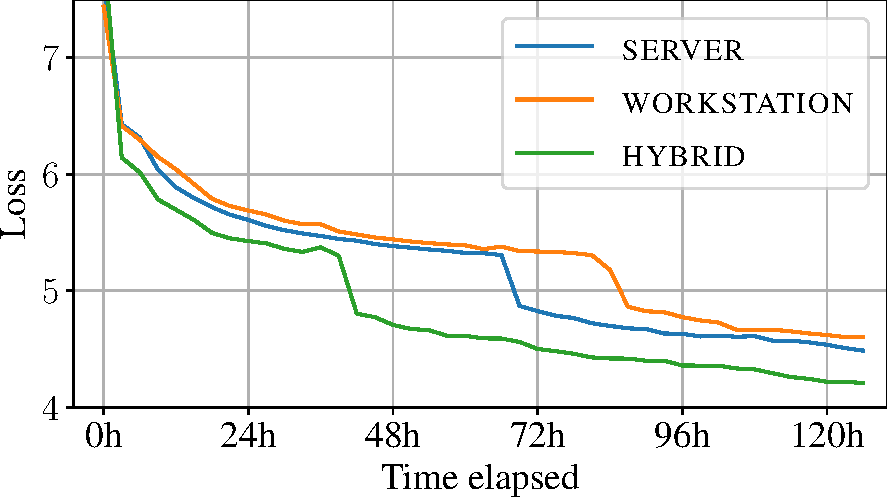
\includegraphics[height=100px]{resources/swav.pdf}
\captionof{figure}{SwAV pretraining performance.}
\label{fig:swav_perf}
\end{minipage}
\begin{minipage}[b][][b]{0.49\textwidth}
\centering
\renewcommand{\arraystretch}{1.2}
\begin{tabular}{lccc}
\toprule
\multicolumn{1}{c}{\multirow{2}{*}{Setup}} & \multicolumn{3}{c}{Algorithm} \\
 & AR & PS & Ours             \\ 
\midrule
A: 8x1Gb/s & \textbf{1.19} & 4.73 & 1.20 \\
B: 16x0.2Gb/s & \textbf{5.3} & 39.6 & \textbf{5.3} \\
C: A + B& 5.69 & 14.1 & \textbf{2.96} \\
D: B + 1x2.5Gb/s & 5.3 & 3.22 & \textbf{3.18} \\
\bottomrule
\end{tabular}
\vspace{8pt}
\captionof{table}{ResNet-50 averaging performance.}
\label{tab:averaging_perf}
\end{minipage}
\vspace{-4pt}

\subsection{Self-supervised pretraining for language understanding}
\label{sect:exp_albert}

Next, we investigate how collaborative training performs for more complex models. In this experiment, we pretrain the ALBERT-large~\cite{albert} masked language model on the WikiText-103 dataset~\cite{wikitext103}. We chose this setup for two reasons: first, ALBERT is very sensitive to the choice of hyperparameters, and specifically batch size, even more than regular Transformers~\cite{trainingtips}. This makes it easier to verify that DeDLOC can reproduce the training conditions of regular data-parallel training. Second, because of weight sharing, training ALBERT is relatively more compute- and less communication-intensive than regular BERT~\cite{bert}, which makes it possible to train with lower bandwidth.
\nocite{paszke2019pytorch}

As before, we follow the exact training configuration from the original paper, but use GPUs instead of TPUs. We use the implementation of ALBERT from the \texttt{transformers} library~\cite{wolf-etal-2020-transformers}. We run all experiments on cloud instances with Tesla T4 GPUs and report the training loss as a function of time, similarly to~\cite{lin2020multinode,switch}. In order to evaluate how DeDLOC performs with different network speeds, we consider the following setups on the same platform with controlled conditions:
\begin{itemize}[leftmargin=*]
   \item \textbf{High-bandwidth:} 16 workers, each with Tesla T4 and 25 Gb/s symmetric bandwidth;
    \item \textbf{Heterogeneous:} same, but with 4x 200 Mb/s, 8x 100 Mb/s and 4x 50 Mb/s bandwidths;
    \item \textbf{Heterogeneous + load balancing:} like Heterogeneous, but with adaptive averaging (Section~\ref{sect:method_algorithm});
    \item \textbf{Auxiliary peers:} the previous setup with 4 additional CPU-only peers at 1 Gb/s bandwidth.
    \item \textbf{Time-varying:} same as previous, but with 8 additional peers at 100 Mb/s. The extra peers are training part-time, jointly alternating between 8 hours of training and 8 hours of downtime.
\end{itemize}
\pagebreak[0]

\begin{minipage}[b][][b]{0.65\textwidth}
\centering
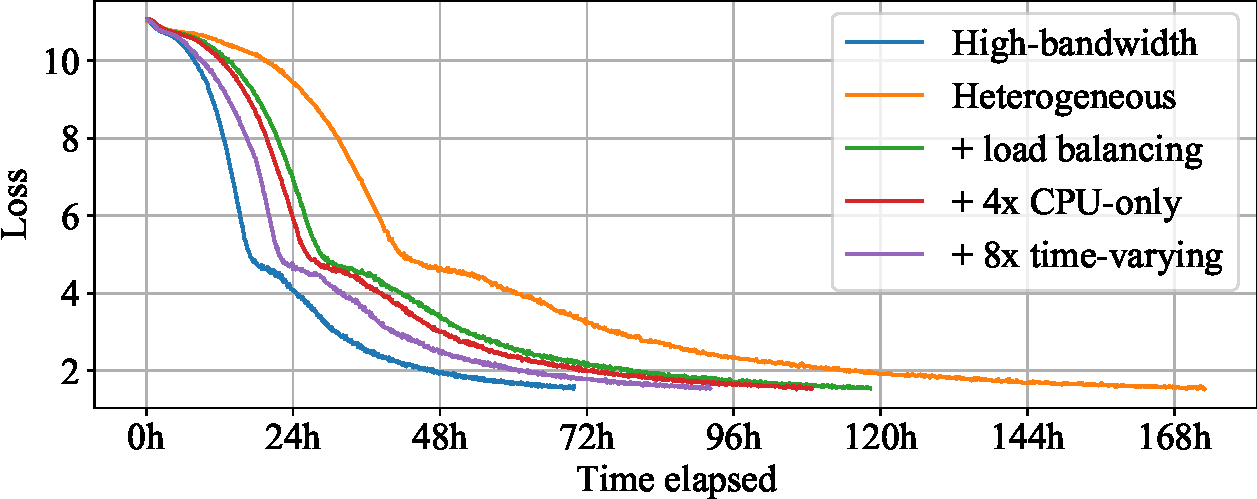
\includegraphics[width=\textwidth]{resources/convergence_albert.pdf}
\vspace{-14pt}
\captionof{figure}{ALBERT pretraining performance.}
\label{fig:albert_perf}
\end{minipage}
\begin{minipage}[b][][b]{0.32\textwidth}
\centering
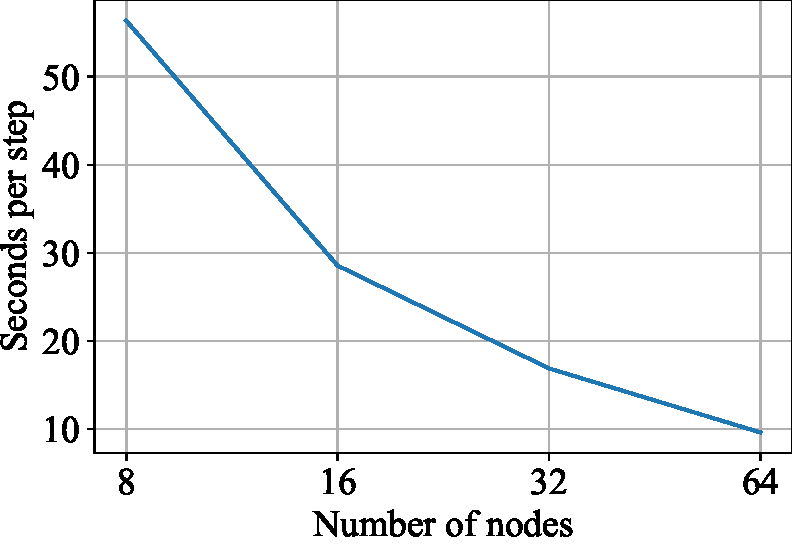
\includegraphics[width=\textwidth]{resources/albert_scalability.pdf}
\vspace{-14pt}
\captionof{figure}{Scalability measurements for ALBERT pretraining.}
\label{fig:albert_scalability}
\end{minipage}

As one can see in Figure~\ref{fig:albert_perf}, naïve training with low-bandwidth peers results in an~$\approx$ 2.5x slowdown compared to high-bandwidth ones. Enabling load balancing accelerates that setup by $\approx47\%$. This effect grows to over 60\% when adding 4 auxiliary peers. Finally, adding 8 part-time peers allows the collaboration to train at 74\% the speed of the high-bandwidth setup without sacrificing the training stability. This turns the latter setup into a viable alternative to traditional distributed training without the need for expensive infrastructure (see the cost analysis in Appendix~\ref{appendix:cost_analysis}). In addition, we demonstrate the high scalability of DeDLOC in Figure~\ref{fig:albert_scalability}, which was obtained by running the same experiment with a varying number of nodes and measuring the time between gradient descent steps. 

\vspace{-6pt}
\subsection{Real-world collaborative training}\label{sect:exp_bengali}
\vspace{-4pt}

For our final evaluation, we organized an actual collaborative training run with volunteer participants, who were asked to pretrain a Transformer masked language model for the Bengali language. This task was chosen deliberately to show the benefits of collaborative training: Bengali has over 230M native speakers who can benefit from recent advances in NLP, but there are few pretrained models available for this language.
We recruited 30 Bengali-speaking volunteers and 10 outside collaborators. All participants received instructions for contributing with free cloud platforms and access to the code for training on local computers. To avoid bias, we did not encourage any specific form of participation: volunteers were free to choose what hardware they contributed and for how long.

Specifically, we trained the ALBERT-large model on Wikipedia and the Bengali part of the OSCAR~\cite{Oscar} multilingual corpus. The model was named sahajBERT after conducting a poll among the participants. We adapted our preprocessing by following the best practices for the Bengali language described in Appendix~\ref{appendix:bn_albert_tokenizer}. To stream from a mix of Wikipedia and OSCAR, the training process iteratively sampled examples from one or the other dataset, as described in Section~\ref{sect:method_system_design}. We accounted for uneven size and quality of data by oversampling Wikipedia by a factor of 2, which resulted in mixing probabilities of 0.23 for Wikipedia and 0.77 for OSCAR. Other hyperparameters were set to the same values as in Section~\ref{sect:exp_albert}. Also, in Appendix~\ref{appendix:xl} we report the results of sahajBERT-XL --- a four times larger model with a specialized architecture that used both GPU and TPU resources.

\begin{figure}[b]
\vspace{-14pt}
% \captionsetup[subfigure]{belowskip=-1pt}
\noindent
\centering
\begin{subfigure}[t]{0.37\textwidth}
\centering
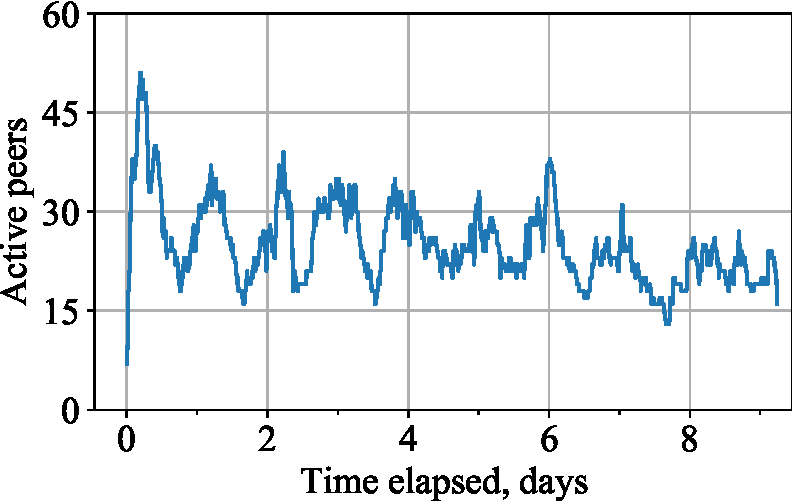
\includegraphics[width=\textwidth]{resources/peer_activity.pdf}
\caption{Collaboration activity.}
\label{fig:activity}
\end{subfigure}
\begin{subfigure}[t]{0.3\textwidth}
\centering
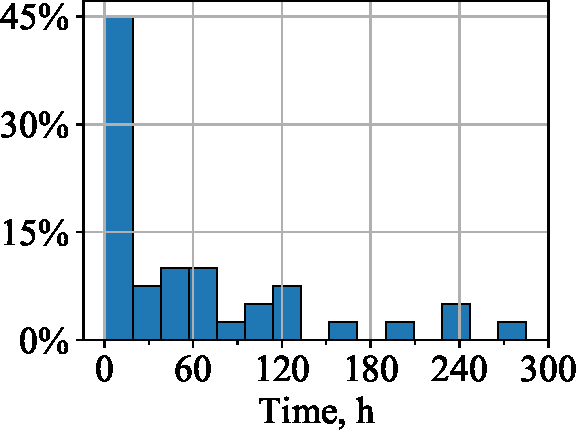
\includegraphics[width=\textwidth]{resources/contrib_hist.pdf}
\caption{Participation time histogram.}
\label{fig:contrib}
\end{subfigure}
\begin{subfigure}[t]{0.3\textwidth}
\centering
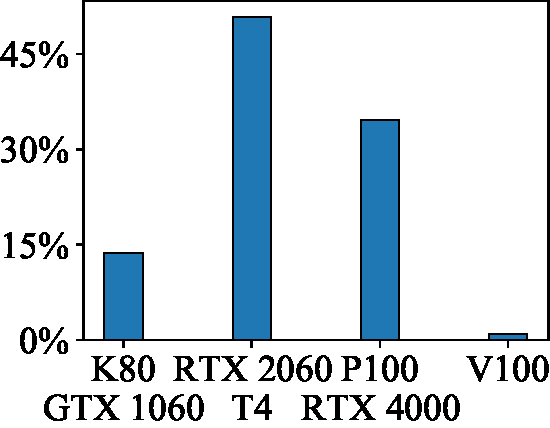
\includegraphics[width=\textwidth]{resources/gpu_hist.pdf}
\caption{Summary of volunteer hardware with example GPUs.}
\label{fig:device}
\end{subfigure}
\vspace{-4pt}
\caption{Collaborative experiment summary.}
\end{figure}


In total, the 40 volunteers contributed compute time from 91 unique devices, most of which were running episodically. Figure~\ref{fig:contrib} shows that although the median GPU time contributed by volunteers across all devices was $\approx$ 1.5 days, some participants ran the training script on several devices, attaining more than 200 hours over the duration of the experiment. With the exception of the start and the end of the collaborative run, the number of simultaneously active devices mostly varied between 15 and 35 depending on the local time. There was less activity in the last 3 days, likely because the volunteers could see that the model has converged on a public Weights \& Biases~\cite{wandb} dashboard.

As depicted in Figure~\ref{fig:device}, individual device performance varied significantly among the collaborators. Along with the resources provided by participants, we also used 16 preemptible single-GPU cloud T4 instances for training.
We have estimated that the average volunteer device consumed 6.95 GB of network traffic per hour of training. While this bandwidth usage is by no means insignificant, it is comparable with cloud gaming~\cite{google_stadia} or high-quality video streaming~\cite{netflix}.

The model converged after 8 days of training, which is 1.8x as fast as regular distributed training with 8 V100 GPUs that we ran as a baseline; Figure~\ref{fig:collab_loss} displays the convergence plots for both setups. At the same time, the stepwise learning curves of the two runs were virtually identical (see Appendix~\ref{appendix:stepwise_learning_curves}), which supports our hypothesis that training with DeDLOC is equivalent to a regular large-batch SGD.
 
\vspace{2pt}
\begin{minipage}[b]{0.49\textwidth}
\centering
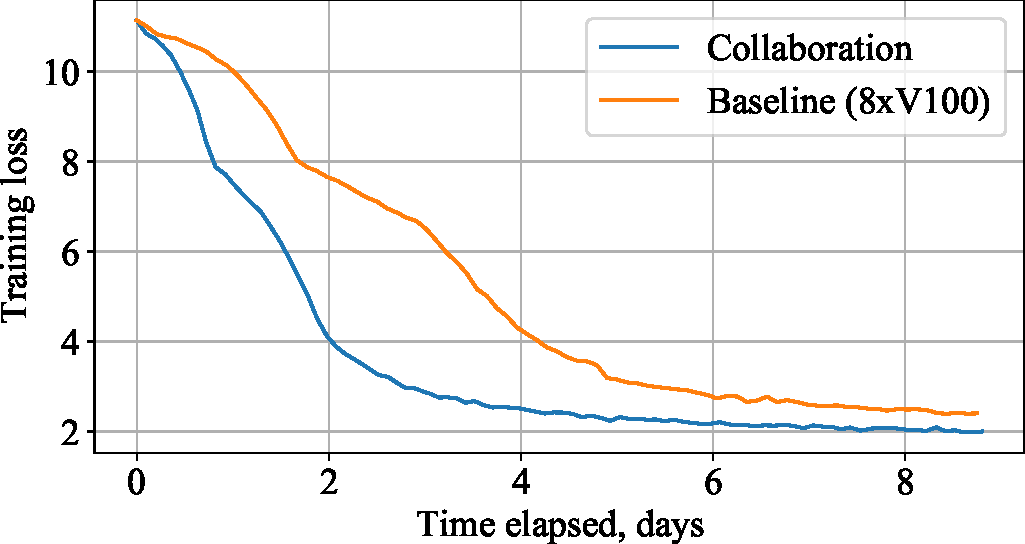
\includegraphics[width=0.95\linewidth]{resources/loss_collab_bengali.pdf}
\vspace{-4pt}
\captionof{figure}{Training progress of sahajBERT.}
\label{fig:collab_loss}
\end{minipage}
\begin{minipage}[b]{0.5\textwidth}
\setlength{\tabcolsep}{2pt}
\renewcommand{\arraystretch}{1.2}
\begin{tabular}{lcc}
\toprule
Model  & Wikiann F1 &NCC Accuracy \\
\midrule
bnRoBERTa           & 82.32 $\pm$ 0.67 &  80.94 $\pm$ 0.45 \\
IndicBERT           & 92.52 $\pm$ 0.45 &  74.46 $\pm$ 1.91 \\
XLM-R               & 96.48 $\pm$ 0.22 &  90.05 $\pm$ 0.38 \\
\midrule
sahajBERT           & 95.45 $\pm$ 0.53 &  91.97 $\pm$ 0.47 \\
sahajBERT-XL        & \bf 96.59 $\pm$ 0.26 & \bf 92.91 $\pm$ 0.43 \\
\bottomrule
\end{tabular}
\captionof{table}{Downstream evaluation results.}
\label{tab:downstream}
\end{minipage}

Finally, we compared the Bengali language representations of sahajBERT with those of other pretrained models on several downstream applications. The first model is XLM-R Large~\cite{xlmr} --- a cross-lingual Transformer-based masked language model that was pretrained on 100 languages and remains a strong baseline for multilingual representation learning. Similarly to sahajBERT, the second model, IndicBERT~\cite{kakwani-etal-2020-indicnlpsuite}, is also based on the ALBERT architecture; however, it was pretrained on 12 languages, including Bengali and Indian English. The third model, bnRoBERTa~\cite{jain2020indictransformers}, is a RoBERTa architecture trained on a monolingual Bengali corpus. We evaluate the model quality on two tasks: WikiANN~\cite{pan-etal-2017-cross} named entity recognition dataset and Soham News Category Classification benchmark from IndicGLUE~\cite{kakwani-etal-2020-indicnlpsuite}. For a detailed description of the setup, refer to Appendix~\ref{appendix:exp_bengali_evaluation}.

As shown in Table~\ref{tab:downstream}, sahajBERT performs comparably to three strong baselines despite being pretrained in a heterogeneous and highly unstable setting.
Notably, our collaboratively trained model outperforms two specialized monolingual baselines and demonstrates competitive results to XLM-R Large, even though the latter has significantly more parameters (560 million instead of 17 million) and was trained on five hundred high-performance data center GPUs instead of tens of low-cost or even free-tier accelerators.
This result confirms previous findings on the benefits of parameter sharing  that were made by authors of ALBERT. Also, it highlights one additional advantage of such architectures: specifically, one can train a high-quality representation model in a communication-constrained setting (for instance, over the Internet) without facing noticeable data transfer bottlenecks.

\vspace{-6pt}
\section{Conclusion and future work}
\vspace{-4pt}
In this work, we propose Moshpit All-Reduce, a decentralized averaging protocol intended for distributed optimization in unstable and network-constrained environments. It has favorable theoretical properties when compared to gossip-based approaches and achieves considerable speedups in distributed training for image classification and masked language modeling.

Our approach was primarily designed for cloud-based training and federated learning, as well as for distributed training on unreliable instances; future work might explore additional settings, such as collaborative training of neural networks.
Another potential research direction is to study the interactions of Moshpit All-Reduce with other methods that improve communication efficiency of distributed optimization, such as gradient compression.
Finally, the idea of arranging All-Reduce nodes into groups can be improved to address specific issues that may arise in practice, such as the varying number of workers and their geographical distribution. 

\vspace{-6pt}
\section*{Acknowledgements}
\vspace{-4pt}
We would like to thank Anastasia Koloskova, Liudmila Prokhorenkova and Anton Osokin for helpful feedback and discussions. We are also grateful to the anonymous reviewers for their suggestions on improving the paper. Finally, we would like to thank Dmitry Afanasiev, Vladimir Aliev, Anand Jayarajan and Michael Solotky for their suggestions on the technical aspects of our study. 
This project was supported in
part by the Canada Foundation for Innovation JELF grant,
NSERC Discovery grant, AWS Machine Learning Research
Award, and Facebook Faculty Research Award. The paper was also partially supported by by a grant for research centers in the field of artificial intelligence, provided by the Analytical Center for the Government of the Russian Federation in accordance with the subsidy agreement (agreement identifier 000000D730321P5Q0002) and the agreement with the Moscow Institute of Physics and Technology dated November 1, 2021 No. 70-2021-00138. The computational resources for the experiments were provided by the Amazon Research Awards program and Yandex.

\bibliographystyle{unsrt}
\bibliography{bibliography}










\clearpage
\part*{Supplementary Material}
\appendix

\section{GPU instance costs}
\label{sect:cloud_costs}

This section provides a brief cost analysis of typical deep learning compute resources both in the cloud and on-premises.
For brevity, we limit this analysis to the popular GPUs available at the time of submission. Note that the exact costs will depend on a variety of factors such as the cloud provider, the region, electricity costs, and market fluctuations. Therefore, we warn the reader to consider this analysis only as a rough estimate. 

Specifically, we estimate the compute costs for the occasional usage scenario: running a single set of experiments over several weeks or conducting infrequent experiments. This scenario covers most research scientists and small organizations. The most straightforward way to provision a GPU server in such a scenario is to rent it from a cloud provider (e.g., GCP or AWS) or a public marketplace (e.g., Vast.ai or Golem).

While the exact server specifications vary from one provider to another, there are two broad categories of GPU machines: regular and preemptible. Regular instance types typically offer 1--8 GPUs per node with tight uptime guarantees (typically $99.99\%$) and a high-bandwidth network (tens of Gb/s). In turn, preemptible instances provide the same resource type at a significant discount with the condition that the machine can be terminated at any time after short notice.

To account for individual variations, we report the average rent price over three popular cloud providers.
We consider three popular instance types: two high-end instances with 8 Tesla V100 or A100 GPUs and a low-end instance with a single Tesla T4 GPU.
We also describe several low-end servers and workstations available on a public marketplace. Unlike cloud VMs, these instances are hosted on non-curated hardware with less uptime guarantees (typically 95\% -- 99.9\%), slower network and significant variation in performance. However, marketplace instances are the cheapest in terms of cost per TFLOPS. To quantify this, we report the average over three most affordable instances that fit the chosen minimum requirements.

As a point of comparison, we also measure each system's training performance for BERT-Large~\cite{bert} fine-tuning on SQuAD v1.1~\cite{squad} in PyTorch with mixed precision. We follow the official benchmarking protocol by~\cite{nvidia_perf} and reuse the official performance results for V100, A100, and T4 instances. The only exception is GTX 1080Ti, where we use full 32-bit precision because that device does not support efficient half-precision operations.

\begin{table}[h]
\small
\setlength{\tabcolsep}{2pt}
\renewcommand{\arraystretch}{1}
\centering
\caption{Cloud and marketplace GPU instance pricing for short-term usage.}
\label{fig:cloud_costs}
\begin{tabular}{@{}ccccccc@{}}
\toprule
\multicolumn{4}{c}{Minimum system specifications} & \multicolumn{2}{c}{Average cost, \$/hour} & \multirow{2}[2]{*}{\shortstack{BERT-Large\\ training samples/s}} \\
\cmidrule(lr){1-4}\cmidrule(lr){5-6}
GPU & CPU cores & CPU type & RAM, GB & Regular & Preemptible &  \\ \midrule
\multicolumn{7}{c}{Cloud instances} \\ \midrule
8$\times$ V100 & 64 & Intel Xeon Broadwell & 480 & 23.47 & 7.13 & 354 \\
8$\times$  A100 & 96 & AMD Epyc ROME & 960 & 30.65 & 10.18 & 755 \\
1$\times$  T4 & 4 & Intel Xeon Cascade Lake & 16 & 0.46 & 0.18 & 18 \\ \midrule
\multicolumn{7}{c}{Marketplace instances} \\ \midrule
6$\times$ 3090 & 32 & AMD Epyc Rome & 480 & 5.04 & 4.17 & 154 \\
4$\times$  2080Ti & 16 & Intel Xeon Haswell & 240 & 0.96 & 0.84 & 83.4 \\
1$\times$  RTX 1080Ti & 8 & Intel Xeon Haswell & 16 & 0.22 & 0.16 & 12 \\ \bottomrule
\end{tabular}
\end{table}

Table~\ref{fig:cloud_costs} shows two main tendencies. First, preemptible \textit{cloud} instances are, on average, three times cheaper than their non-preemptible counterparts\footnote{The cost can be up to $11{\times}$ cheaper for some instance types, e.g. Azure V100 instances in the central US region at the time of writing.}. Second, the high-end HPC-grade servers that offer the highest raw performance are less cost-effective than lower-tier servers and marketplace instances. In theory, one could match the raw floating-point performance of a $8{\times}$V100 instance at a fraction of its cost using multiple lower-tier workstations, such as $4{\times}$ RTX 2080Ti, with a smaller total cost.
However, in practice, running distributed training with these workstations is challenging due to their unreliability and slow network connection.

Note that this analysis does not represent the cloud costs for sustained GPU usage. If an organization plans to constantly use GPU resources over a period of multiple years, they can reduce the costs by deploying their own compute infrastructure or relying on the sustained usage discounts reaching up to 60--70\%. Thus, the long-term compute costs are much harder to analyze and depend on a number of additional factors, such as local electricity prices for on-premise infrastructure. However, this scenario offers similar trade-offs: HPC-grade infrastructure offers greater interconnectivity, but requires expensive network interface cards, high-end switches and a more complex setup process.

\section{Additional Related Work}
\label{sect:post_related}

In this section, we review some of the papers relevant to our work, but omitted from the main part due to space constraints. 

\subsection{Decentralized training}\label{sect:post_related_gossip}
In this subsection, we give additional details about the dependence of gossip-based optimization methods on the spectral properties on the communication graph through the spectral properties of the mixing matrix~\cite{xiao2004fast,scaman2019optimal} or the Laplacian matrix~\cite{merris1994laplacian,uribe2020dual} of the network. 
That is, gossip finds approximate average on nodes with accuracy $\varepsilon$ after $\cO\left((1-\lambda_2(\mM))^{-1}\log(\varepsilon^{-1})\right)$ iterations, where $\mM$ is the mixing matrix and $\lambda_2(\mM)$ is the second largest eigenvalue of $\mM$ when sorted by absolute value. 
The quantity $\eta = 1-\lambda_2(\mM)$ is called the spectral gap of the mixing matrix $\mM$, and $\eta^{-1}$ is typically a polynomial of the total number of nodes $N$ when the maximal degree of the node is $\cO(1)$. For example, for uniformly averaging $\mM$ one can show that $\eta^{-1} = \cO(N^2)$ for the ring topology (node degree $2$), $\eta^{-1} = \cO(N)$ for the two-dimensional torus topology (node degree  $2$), and $\eta^{-1} = \cO(1)$ for the fully connected graph (node degree $N-1$); one can find more examples in~\cite{aldous2002reversible}. Similarly, the communication complexity of decentralized optimization methods often has multiplicative dependence on either $\cO(\eta^{-1})$ (see~\cite{xu2020distributed} and references therein) or $\cO(\eta^{-\nicefrac{1}{2}})$~\cite{scaman2019optimal,uribe2020dual,fallah2019robust,kovalev2020optimal}, which is not improvable for gossip-based methods~\cite{arjevani2015communication,scaman2017optimal}.

Contrary to this, Moshpit All-Reduce does not depend on a fixed communication graph and the properties of its mixing matrix.
However, it depends on the number of averaging groups and the total number of peers (see Theorem~\ref{thm:quality_of_avg_deterministic_vectors}), which can be viewed as properties of a time-varying random communication graph. Fortunately, this dependence is often much better than in gossip: as we mentioned in the main part of the paper, even if workers are randomly split into pairs at each iteration, the simplified version of Moshpit All-Reduce makes the average distortion (the left-hand side of Equation~\ref{eq:determ_quality_of_avg}) at least $2$ times smaller after each round on average.

\subsection{Compressed communication}
Another popular approach to address the communication bottleneck is communication compression~\cite{seide20141,alistarh2017qsgd,suresh2017distributed, ramezani2021nuqsgd, faghri2020adaptive}: before sending any information (e.g., iterates, gradients, Hessians or more sophisticated data) over the network, peers compress this information by applying a possibly random transformation. As the result, peers send fewer bits for each communication round, but the total number of communication rounds needed to achieve the predefined accuracy of the solution increases. However, compression can be useful in situations when the reduction in communication costs of one round is more important than the increase in the number of these rounds~\cite{horvath2019natural}.

There are two distinct groups of works on distributed training with compressed communication: ones that focus on unbiased compression operators (e.g., Rand-K, $\ell_p$-quantization) and ones studying algorithms with biased compressors (e.g., Top-K); see a detailed summary of  popular compression operators in~\cite{beznosikov2020biased}). 
Quantized SGD (QSGD)~\cite{alistarh2017qsgd} and TernGrad~\cite{wen2017terngrad} were among the first compression methods with convergence guarantees. Next, the convergence analysis of these methods was generalized and tightened in the (strongly) convex case in~\cite{mishchenko2019distributed}. Moreover, the authors of \cite{mishchenko2019distributed} proposed a modification of QSGD called DIANA: this algorithm is based on the quantization of gradients' differences, which helps it achieve linear convergence in the strongly convex case when peers compute full gradients. Next, DIANA was generalized to arbitrary unbiased compression in~\cite{horvath2019stochastic}, where authors also developed and analyzed the variance-reduced version of DIANA. After that, several further modifications, such as Accelerated DIANA~\cite{li2020acceleration} and DIANA with bidirectional compression~\cite{gorbunov2020linearly,philippenko2020artemis}, were proposed. Finally, we refer the reader to~\cite{li2020unified,haddadpour2020federated,das2020improved, pmlr-v139-gorbunov21a} for state-of-the-art results for distributed methods with unbiased compression in the non-convex case.

However, naïve application of biased compression operators can lead to significantly worse performance in practice. For instance, as it was shown recently in~\cite{beznosikov2020biased}, parallel SGD with Top-1 compression can diverge exponentially fast. Therefore, biased compressors are used jointly with so-called error-compensation~\cite{seide20141}. The first analysis of Error-Compensated SGD (EC-SGD) was proposed in~\cite{stich2018sparsified,karimireddy2019error} which then was generalized and tightened in~\cite{beznosikov2020biased}. Next, several further improvements, such as an accelerated version of EC-SGD~\cite{qian2020error} and linearly converging EC-SGD~\cite{gorbunov2020linearly}, were recently proposed. However, current theory does not show any superiority of distributed methods with biased compressors to the ones with unbiased compression operators.
In addition, one can combine decentralized communication with compression. Such combinations with unbiased compression operators were studied in~\cite{reisizadeh2019exact,kovalev2020linearly} and with biased operators in~\cite{pmlr-v97-koloskova19a,Koloskova2020Decentralized}.
In this paper, we do not study the interaction of different compression methods and Moshpit Averaging, leaving this promising direction to future work.

\subsection{Multiple local steps}
Alternatively, to reduce the impact of the communication bottleneck, it is possible to perform several local optimization steps on each peer between the communication rounds.
This approach is based on the idea that the increased computational load of peers will decrease the number of communication rounds required to obtain the optimal parameters; it is frequently used in federated learning~\cite{konevcny2016federated,kairouz2019advances}. In particular, one of the most popular methods with multiple local steps is called Local-SGD or Federated Averaging~\cite{konevcny2016federated,Stich18local}. The first results on its convergence were given in \cite{Stich18local,LinSPJ2018local}, and later they were tightened and generalized both for homogeneous~\cite{khaled2020tighter,woodworth2020local} and heterogeneous  cases~\cite{khaled2020tighter,woodworth2020minibatch}. Recently, further modifications of Local-SGD were proposed and analyzed: these modifications include acceleration \cite{yuan2020federated}, variance reduction \cite{gorbunov2020local}, communication compression \cite{basu2019qsparse,haddadpour2020federated,das2020improved}, decentralization \cite{li2019communication,koloskova2020unified}, adaptive and proximal methods \cite{reddi2021adaptive,yuan2020federated_comp}, and resistance to client drift \cite{karimireddy2020scaffold}.
Moshpit SGD can perform multiple local gradient steps before synchronization by design, as shown in Algorithm~\ref{alg:moshpit_local_sgd}.


\subsection{Asynchronous methods}
In the previous subsections, we mostly discussed synchronous distributed methods, since they are more widespread and better studied than asynchronous ones. Mainly, this is because asynchronous methods are more difficult to implement, debug and analyze under general assumptions. However, such methods can be more efficient in terms of using computational resources, which leads to faster wall-clock convergence \cite{assran2020advances}. In recent years, several asynchronous stochastic methods~\cite{recht2011hogwild,zhao2016fast,leblond2017asaga}, methods with no shared memory~\cite{peng2016arock,mishchenko2018delay}, and methods with delayed updates~\cite{agarwal2011distributed,feyzmahdavian2016asynchronous,arjevani2020tight,gorbunov2020linearly} were proposed and analyzed: one can find more details in a recent survey~\cite{assran2020advances}.
Moshpit SGD belongs to this family of asynchronous approaches as well, because the averaging steps happen in smaller groups and can be interleaved with local parameter updates.

\subsection{Distributed Hash Tables}
\label{sect:related_dht}

In this work, we set out to improve distributed averaging with a dynamic matchmaking protocol. Without a central server, this protocol relies on decentralized data structures to organize peers. The main data structure we use is the Distributed Hash Table, or DHT. On a high level, DHT is a distributed fault-tolerant ``dictionary'' that can be accessed by every participant. Each key-value pair is stored on a subset of peers determined by the $\mathrm{hash}$ function of the key.

Each participant has a unique identifier (ID) sampled uniformly from the $\mathrm{hash}$ function output range. When storing a $(key,\ value)$ pair, one must find $k$ peers whose IDs are nearest to $\mathrm{hash}(key)$ according to a chosen metric. After that, the participant requests each of those peers to store $(key,\ value)$. When retrieving a value for a key, one should compute $\mathrm{hash}(key)$, search for peers with IDs nearest to that $\mathrm{hash}$ value and request the value from those peers.

Specific DHT versions, such as Chord~\cite{chord} or Kademlia~\cite{kademlia}, employ different hash types and algorithms for finding nearest peers. For instance, Kademlia DHT sorts peers based on the XOR distance function: $d(x, y) = \mathrm{int}(x \oplus y)$.

In DHT, each participant is directly aware of only a small subset of peers. When storing or retrieving a key, the participant requests additional peers from its neighbors in a semi-greedy search, minimizing the XOR distance until it finds $k$ nearest peers. In Kademlia, nodes form a special navigable graph structure that lets them find nearest peers in at most $\cO(k + \log N)$ requests to other peers, where $N$ is the total number of participants. Due to their scalability and fault-tolerance, DHTs found numerous applications including BitTorrent, Ethereum, I2P and decentralized deep learning~\cite{learning_at_home}.

\section{Proofs of Mixing Properties of Moshpit All-Reduce}\label{sect:missing_proofs}

\textbf{Notation.} Throughout the following sections, we use the standard notation from the literature on stochastic optimization. That is, for any $n$-dimensional vectors $x = (x_1,\ldots,x_n)^\top,y = (y_1,\ldots,y_n)^\top\in\R^n$ we use $\langle x,y\rangle$ to denote the standard inner product: $\langle x, y\rangle = x_1y_1 + \ldots + x_ny_n$. Next, we use $\|x\|$ to denote the $\ell_2$=norm of $x$ ($\|x\| = \sqrt{\langle x, x\rangle}$), $\EE[\xi]$ to denote an expectation of a random variable $\xi$, $\EE[\xi\mid \eta]$ is used for the conditional expectation of $\xi$ given $\eta$, and $\PP\{E\}$ denotes the probability of an event $E$.

\subsection{Computing exact average in a full grid}\label{sect:equiv_to_torus}
As discussed in Section~\ref{sect:method_algorithm}, Moshpit All-Reduce obtains the exact average of parameter vectors from $N$ peers arranged in a grid with $d$ coordinates and $M$ positions per coordinate when $N\equiv M^d$. That is, when the grid is full and each step averages $M$ parameter values along a single grid coordinate without repetitions, the algorithm needs only $d$ steps to compute the actual average across all nodes. In this section, we give a proof of this fact.

First, let us formally define the setting and the averaging steps of Moshpit All-Reduce in this specific case. Let $\theta_{i_1 i_2\ldots i_d}$ be the parameter vector of the worker with coordinates $i_1, i_2,\ldots, i_d$; each coordinate $i_k$ takes values from $1$ to $M$, because the hypercube of peers is completely full (thus, due to the pigeonhole principle, there are no unoccupied coordinates). Next, arrange the coordinates of these vector according to the order of averaging iterations: namely, at iteration 1
\begin{equation}
    \overline{\theta}_{i_1 i_2\ldots  i_d}^1=\frac{1}{M}\sum_{j_1=1}^M \theta_{j_1 i_2\ldots i_d},\quad  i_1\in\{1,\ldots,M\},
\end{equation}
which means that for the first iteration, we take the average across the first axis $\overline{\theta}^1$ and replicate it across all $M$ resulting vectors regardless of their index $i_1$. The next averaging steps can be expressed similarly with a simple recurrence relation:
\begin{equation}
\label{eqn:avg_recurrence}
    \overline{\theta}_{i_1 i_2 \ldots i_d}^t=\frac{1}{M}\sum_{j_t=1}^M \overline{\theta}_{i_1\ldots i_{t-1} j_t i_{t+1}\ldots i_d}^{t-1}.
\end{equation}
Given this formal definition, we can now state and prove the exact averaging result:
\begin{theorem}[Exact average in a full $d$-dimensional hypercube after $d$ steps]
Assume that $M^d$ peers are arranged in a $d$-dimensional hypercube with $M$ positions in each dimension. Also, assume that each peer fully participates in every averaging step and $M$-sized groups for each averaging iteration are determined based on the hypercube coordinates. Then, if Moshpit All-Reduce is ran in the above setup for $d$ iterations without repeating groups (i.e. averaging across each dimension exactly once), its result for each participant is the average value of $\theta$ across all $M^d$ peers.
\end{theorem}
\begin{proof}
We can directly obtain the expression for the average by expanding the recurrence and rearranging the sums:
\begin{eqnarray*}
    \overline{\theta}_{i_1 i_2\ldots i_d}^d &=& \frac{1}{M}\sum_{j_d=1}^M\overline{\theta}_{i_1\ldots i_{d-1} j_d}^{d-1}=\frac{1}{M}\sum_{j_d=1}^M\left(\frac{1}{M}\sum_{j_{d-1}=1}^M \overline{\theta}_{i_1 i_2\ldots j_{d-1}j_d}\right)=\ldots\\
    &=& \frac{1}{M}\Bigg(\underbrace{\sum_{j_d=1}^M\Bigg(\frac{1}{M}\sum_{j_{d-1}=1}^M\ldots\sum_{j_2=1}^M\Bigg(\frac{1}{M}\sum_{j_1=1}^M}_{d\textrm{ summations}} \theta_{j_1 \ldots j_d}\Bigg)\Bigg)\Bigg)\\
    &=& \frac{1}{M^d}\sum_{j_d=1}^M\sum_{j_{d-1}=1}^M\ldots\sum_{j_2=1}^M\sum_{j_1=1}^M \theta_{j_1 \ldots j_d} =\frac{1}{M^d}\sum_{j_1, \ldots, j_d=1}^M  \theta_{j_1 \ldots j_d}.
\end{eqnarray*}
But this is exactly the global average of all $\theta$, since there are $M^d$ participants and each vector is represented in the sum because of summation over all possible indices.
\end{proof}

Notice that for a given grid of peers, if some of its indices do not have corresponding parameter vectors, Equation~\ref{eqn:avg_recurrence} may result in different average vectors on different workers due to different numbers of peers along a coordinate for different indices. For example, running two iterations of Moshpit Averaging with $d=2,\ M=2$ and three parameter vectors $\theta_{11},\ \theta_{21},\ \theta_{22}$ results in $\frac{\theta_{11}+\theta_{21}}{2}$ on the first worker and $\frac{\theta_{11}+\theta_{21}}{4}+\theta_{22}$ on other workers, with neither equal to the global average. However, the variance of the averaged vectors does decrease, which is formally proven in Section~\ref{sec:proof_quality_of_avg_deterministic_vectors}.

\subsection{Proof of Theorem~\ref{thm:quality_of_avg_deterministic_vectors_0}}\label{sect:correctness_proof}
Below we provide the complete proof of Theorem~\ref{thm:quality_of_avg_deterministic_vectors_0}. For the readers' convenience, we restate the theorem.
\begin{theorem}[Theorem~\ref{thm:quality_of_avg_deterministic_vectors_0}]\label{thm:quality_of_avg_deterministic_vectors_0_supp}
If all workers have non-zero probability of successfully running a communication round in Moshpit Averaging and the order of $\texttt{peers}_t$ is random, then all local vectors $\theta^t_i$ converge to the global average with probability $1$:
\begin{equation}
    \forall i = 1,\ldots, N\quad \left\|\theta^t_i - \frac1N \sum_{i=1}^N \theta^0_i\right\|^2 \xrightarrow[t\to\infty]{} 0.\label{eq:quality_of_avg_deterministic_vectors_0_supp}
\end{equation}
\end{theorem}
\begin{proof}[Proof of Theorem~\ref{thm:quality_of_avg_deterministic_vectors_0}]
    First of all, we notice that \eqref{eq:quality_of_avg_deterministic_vectors_0_supp} is equivalent to
    \begin{equation}
    \forall i = 1,\ldots, N,\;\forall j=1,\ldots,n\quad \left(\theta^t_i(j) - \frac1N \sum_{i=1}^N \theta^0_i(j)\right)^2 \xrightarrow[t\to\infty]{} 0,\label{eq:quality_of_avg_deterministic_vectors_0_supp_tech_1}
    \end{equation}
    where $\theta_i^t(j)$ denotes $j$-th component of $\theta_i^t$. Consider an arbitrary component $j \in \{1,\ldots,n\}$ and the sequence of intervals $\{I_{j,t}\}_{t\ge 0}$ where $I_{j,t} = \text{conv}\{\theta_1^t(j),\theta_2^t(j),\ldots, \theta_N^t(j)\}$. Then, $\{I_{j,t}\}_{t\ge 0}$ is a sequence of nested intervals ($I_{j,t+1} \subseteq I_{j,t} \forall t\ge 0$), since averaging in groups does not expand the convex hull of $\{\theta_1^t,\theta_2^t,\ldots, \theta_N^t\}$. For convenience, we specify the bounds of the intervals: $I_{j,t} = [a_{j,t}, b_{j,t}]$. Using the Cantor's intersection theorem, we conclude that
    \begin{equation*}
        \bigcap\limits_{t=0}^\infty I_{j,t} = I_j = [a_j, b_j],
    \end{equation*}
    where $\overline{\theta}(j) = \frac{1}{N}\sum_{i=1}^n\theta_i^0(j) \in [a_j, b_j]$. If $[a_j, b_j] = \{\overline{\theta}(j)\}$ with probability $1$, then \eqref{eq:quality_of_avg_deterministic_vectors_0_supp_tech_1} holds with probability $1$ as well. Suppose the opposite: there exist such $j \in \{1,\ldots,n\}$, $[a,b]$ and $\delta,\Delta > 0$ that $\overline{\theta}(j) \in [a,b]$, $b-a = \Delta$ and
    \begin{equation*}
        \PP\Bigg\{\underbrace{[a,b] \subseteq \bigcap\limits_{t=0}^\infty I_{j,t}}_{E}\Bigg\} = \delta > 0\quad \text{ and }\quad \forall \varepsilon > 0\; \PP\Bigg\{\underbrace{[a-\varepsilon,b+\varepsilon] \subseteq \bigcap\limits_{t=0}^\infty I_{j,t}}_{E_{\varepsilon}}\Bigg\} < \delta.
    \end{equation*}
    This implies that for all $\varepsilon > 0$ there exists such $T_{\varepsilon} > 0$ that
    \begin{equation*}
        \PP\Big\{\underbrace{\forall t \ge T_{\varepsilon}\;\; a_{j,t}\in [a-\varepsilon,a], b_{j,t}\in[b,b+\varepsilon]}_{E_{\varepsilon}'}\Big\} = \delta_{\varepsilon} > 0.
    \end{equation*}
    Consider $\varepsilon = \frac{\Delta}{(2N+100)^{2N}}$ and assume that the event $E_{\varepsilon}'$ holds. Next, we introduce new notation: $J_{\text{left}}^t = \{i \in \{1,\ldots, n\}\mid \theta_{i}^t(j) \in [a-\varepsilon,a]\}$ and $J_{\text{right}}^t = \{i \in \{1,\ldots, n\}\mid \theta_{i}^t(j) \in [b,b+\varepsilon]\}$. Since $E_{\varepsilon}'$ holds the sets $J_{\text{left}}^t$ and $J_{\text{right}}^t$ are non-empty for all $t\ge T_{\varepsilon}$ with probability $\delta_{\varepsilon} > 0$:
    \begin{equation}
        \PP\left\{\forall t \ge T_{\varepsilon}\;\; J_{\text{left}}^t \neq \varnothing\text{ and }  J_{\text{right}}^t \neq \varnothing\right\} = \delta_{\varepsilon} > 0. \label{eq:quality_of_avg_deterministic_vectors_0_supp_tech_2}
    \end{equation}
    We notice that every pair of workers $i_1,i_2$ has a non-zero probability of taking part in the averaging inside the common group at each iteration since all workers have a non-zero probability of successfully running a communication round and the order of $\texttt{peers}_t$ is random. This implies that every pair of workers $i_1,i_2$ with probability $1$ take part in the averaging inside the common group infinitely many times when $t$ goes to the infinity.
    
    Next, we choose some $t_0 \ge T_{\varepsilon}$. Let $J_{\text{left}}^{t_0} = \{i_{l,1},\ldots, i_{l,q_l}\}$ and $J_{\text{right}}^{t_0} = \{i_{r,1},\ldots, i_{r,q_r}\}$. Consider the event $E_{\varepsilon,0}' \subseteq E_{\varepsilon}'$ such that in $E_{\varepsilon,0}'$ peer $i_{l,1}$ computes an average in the group containing any peer from $J_{\text{right}}^{t_0}$ at some iteration $t_1 > t_0$. Our observations above imply that $\PP\{E_{\varepsilon,0}'\} = \PP\{E_{\varepsilon}'\} = \delta_{\varepsilon} > 0$. Then, $\theta_{i_{l,1}}^{t_1}(j) \ge \frac{N-1}{N}(a-\varepsilon) + \frac{1}{N}b = a-\varepsilon + \frac{1}{N}(\Delta + \varepsilon) = a - \frac{\Delta}{(2N+100)^{2N}} + \frac{1}{N}\left(\Delta + \frac{\Delta}{(2N+100)^{2N}}\right) > a + \frac{\Delta}{2N}$, i.e., $\theta_{i_{l,1}}^{t_1}(j) \in (a,b]$ meaning that $i_{l,1} \not\in J_{\text{left}}^{t_1}$. The last part of the proof shows that for any $t\ge t_1$, the peer $i_{l,1}$ will never be the part of $J_{\text{left}}^t$ and after a finite number of iterations $J_{\text{left}}^t = \varnothing$ with probability $\delta_{\varepsilon} > 0$ when $E_{\varepsilon,0}'$ holds, implying the contradiction with \eqref{eq:quality_of_avg_deterministic_vectors_0_supp_tech_2}.
    
    To show that, we consider the following set of peers: $\widehat{J}_{\text{left}}^{t_1} = \{i\in\{1,\ldots,n\}\mid \exists t \ge t_1:\; \theta_i^{t}(j)\in [a-\varepsilon, a+\frac{\Delta}{2N})\}$. Next, we consider the event $E_{\varepsilon,1}'\subseteq E_{\varepsilon,0}'$ such that in $E_{\varepsilon,1}'$ peer $i_{l,1}$ computes an average in the group containing some peer $i_{l,avg,1}$ from $\widehat{J}_{\text{left}}^{t_1}$ at some iteration $t_2 > t_1$ (and $t_2$ is the first such moment after $t_1$). Again, our observations imply $\PP\{E_{\varepsilon,1}'\} = \PP\{E_{\varepsilon,0}'\} = \delta_{\varepsilon}>0$. Then, $\theta_{i_{l,1}}^{t_2}(j) = \theta_{i_{l,avg,1}}^{t_2}(j) > \frac{N-1}{N}(a-\varepsilon) + \frac{1}{N}\left(a+\frac{\Delta}{2N}\right) = a + \frac{\Delta}{2N^2} - \frac{(N-1)\Delta}{N(2N+100)^{2N}} > a + \frac{\Delta}{4N^2}$. After that, we consider the event $E_{\varepsilon,2}'\subseteq E_{\varepsilon,1}'$ such that in $E_{\varepsilon,2}'$ peer $i_{l,1}$ or $i_{l,avg,1}$ computes an average in the group containing a peer $i_{l,avg,2}\neq i_{l,avg,1}$ from $\widehat{J}_{\text{left}}^{t_1}$ at an iteration $t_3 > t_2$ (and $t_3$ is the first such moment after $t_2$). Then, $\theta_{i_{l,1}}^{t_3}(j), \theta_{i_{l,avg,1}}^{t_3}(j)$ and $\theta_{i_{l,avg,2}}^{t_3}(j)$ are greater than $\frac{N-1}{N}(a-\varepsilon) + \frac{1}{N}\left(a + \frac{\Delta}{4N^2}\right) = a + \frac{\Delta}{4N^3} - \frac{(N-1)\Delta}{N(2N+100)^{2N}} > a + \frac{\Delta}{8N^3}$.
    
    Therefore, after at least $N-1$ of such averaging iterations, with probability $\delta_\varepsilon$ all $\theta_i^t(j)$ will be greater than $a + \frac{\Delta}{(2N)^N} > a$ while $E_{\varepsilon}'$ holds. This contradicts \eqref{eq:quality_of_avg_deterministic_vectors_0_supp_tech_2}. Therefore, 
    \begin{equation*}
        \bigcap\limits_{t=0}^\infty I_{j,t} = \{\overline{\theta}(j)\}
    \end{equation*}
    with probability $1$, which concludes the proof.
\end{proof}


\subsection{Proof of Theorem~\ref{thm:quality_of_avg_deterministic_vectors}}\label{sec:proof_quality_of_avg_deterministic_vectors}
In this section, we provide the complete proof of Theorem~\ref{thm:quality_of_avg_deterministic_vectors}. For convenience, we restate the theorem below.
\begin{theorem}[Theorem~\ref{thm:quality_of_avg_deterministic_vectors}, averaging convergence rate]\label{thm:quality_of_avg_deterministic_vectors_supp}
    Consider the modification of Moshpit All-Reduce that works as follows: at each iteration $k\geq 1$ 1) peers are randomly split into $r$ disjoint groups of sizes $M_1^k,\ldots, M_r^k$ in such a way that $\sum_{i=1}^r M_i^k = N$ and $M_i^k \ge 1\  \forall i = 1,\ldots,r$ and 2) peers from each group compute their group average via All-Reduce. Let $\theta_1,\ldots,\theta_N$ be the input vectors of this procedure and $\theta_1^T,\ldots,\theta_N^T$ be the outputs after $T$ iterations. Then,
    \begin{eqnarray}
         \EE\left[\frac{1}{N}\sum\limits_{i=1}^N\|\theta_i^T - \overline{\theta}\|^2\right] = \left(\frac{r-1}{N} + \frac{r}{N^2}\right)^T\cdot\frac{1}{N}\sum\limits_{i=1}^N\|\theta_i - \overline{\theta}\|^2, \label{eq:determ_quality_of_avg_supp}
    \end{eqnarray}
    where $\overline{\theta} = \frac{1}{N}\sum_{i=1}^N\theta_i$.
\end{theorem}
\begin{proof}
First of all, let us clarify the procedure of random splitting of peers in $r$ groups. We assume that at iteration $k$ of the modified algorithm we generate a random permutation $\pi^k = (\pi_1^k,\ldots,\pi_N^k)$ of $1,\ldots, N$. Next, $J_1^k = \{\pi_1^k,\ldots,\pi_{M_1^k}^k\}$ form the indices of the first group of workers, $J_2^k = \{\pi_{M_1^k+1}^k,\ldots,\pi_{M_2^k}^k\}$ are the indices of the second group, and $J_r^k = \{\pi_{M_1^k+M_2^k+\ldots+M_{r-1}^k+1}^k,\ldots,\pi_{N}^k\}$ are the indices of group $r$. In other words, we generate a random permutation and take contiguous subgroups of indices corresponding to predefined group sizes $M_i^k$, starting from the first group.

By definition, we have $\bigsqcup_{i=1}^r J_i^k = \{1,2,\ldots,N\}$, where $\sqcup$ defines the disjoint union operator. Moreover, notice that group sizes $M_1^k,\ldots,M_r^k$ can depend on $k$ and even be random: for our analysis, it is sufficient that the randomness defining the permutation is independent from $M_1^k,\ldots,M_r^k$. Next, vectors $\theta_1^k,\ldots,\theta_N^k$ are obtained by the following formula:
\begin{equation*}
    \forall j=1,\ldots,N,\quad \theta_j^k = \frac{1}{M_i^k}\sum\limits_{t\in J_i^k}\theta_t^{k-1},\quad \text{where } J_i^k \text{ is the group for which } j\in J_i^k.
\end{equation*}
Using this, we show that the average of vectors $\{\theta_i^k\}_{i=1}^n$ remains the same throughout the iterations of Moshpit All-Reduce:
\begin{equation*}
    \frac{1}{N}\sum\limits_{j=1}^N\theta_j^k = \frac{1}{N}\sum\limits_{i=1}^rM_i^k\cdot\frac{1}{M_i^k}\sum\limits_{t\in J_i^k}\theta_t^{k-1} = \frac{1}{N}\sum\limits_{i=1}^r\sum\limits_{t\in J_i^k}\theta_t^{k-1} = \frac{1}{N}\sum\limits_{j=1}^N\theta_j^{k-1}.
\end{equation*}
Therefore, the quantity $\frac{1}{N}\sum_{j=1}^N\|\theta_j^k - \overline{\theta}\|^2$ (average distortion) measures the quality of averaging. For this quantity, we can derive the following expression:
\begin{eqnarray}
    \frac{1}{N}\sum\limits_{j=1}^N\|\theta_j^k - \overline{\theta}\|^2 &=& \frac{1}{N}\sum\limits_{i=1}^r M_i^k\left\|\frac{1}{M_i^k}\sum\limits_{t\in J_i^k}\theta_t^{k-1} - \overline{\theta}\right\|^2\notag\\
    &=& \frac{1}{N}\sum\limits_{i=1}^r\frac{1}{M_i^k}\left(\sum\limits_{t\in J_i^k}\|\theta_t^{k-1} - \overline{\theta}\|^2 + 2\sum\limits_{t,l\in J_i^k, t < l}\langle \theta_t^{k-1} - \overline{\theta}, \theta_l^{k-1} - \overline{\theta} \rangle\right).\notag
\end{eqnarray}
Taking the expectation $\EE_{\pi^k}[\cdot]$ with respect to the randomness coming from the choice of $\pi^k$ we get
\begin{eqnarray}
    \EE_{\pi^k}\left[\frac{1}{N}\sum\limits_{j=1}^N\|\theta_j^k - \overline{\theta}\|^2\right] &\notag\\
    &\hspace{-2.5cm}= \frac{1}{N}\sum\limits_{i=1}^r\frac{1}{M_i^k}\left(\EE_{\pi^k}\left[\sum\limits_{t\in J_i^k}\|\theta_t^{k-1} - \overline{\theta}\|^2\!\right] \!+\! 2\EE_{\pi^k}\!\left[\sum\limits_{t,l\in J_i^k, t < l}\langle \theta_t^{k-1} - \overline{\theta}, \theta_l^{k-1} - \overline{\theta} \rangle\right]\right).\notag
\end{eqnarray}
Since $\forall j,j_1,j_2 \in\{1,\ldots,N\},j_1\neq j_2$ and for all $i=1,\ldots,r$
\begin{equation*}
    \PP\left\{j\in J_i^k\right\} = \frac{M_i^k}{N},\quad \PP\left\{j_1,j_2 \in J_i^k\right\} = \frac{M_{i}^k(M_i^k - 1)}{N^2},
\end{equation*}
we have
\begin{eqnarray*}
    \EE_{\pi^k}\left[\frac{1}{N}\sum\limits_{j=1}^N\|\theta_j^k - \overline{\theta}\|^2\right] &=& \frac{1}{N}\sum\limits_{i=1}^r\frac{1}{N}\sum\limits_{j=1}^N\|\theta_j^{k-1} - \overline{\theta}\|^2\\
    &&\quad +\frac{1}{N}\sum\limits_{i=1}^r2\frac{M_i^k - 1}{N^2}\sum\limits_{1 \le j_1 < j_2 \le N}\langle \theta_{j_1}^{k-1} - \overline{\theta}, \theta_{j_2}^{k-1} - \overline{\theta}\rangle\\
    &=& \frac{r}{N^2}\sum\limits_{j=1}^N\|\theta_j^{k-1} - \overline{\theta}\|^2 + 2\frac{N-r}{N^3}\sum\limits_{1 \le j_1 < j_2 \le N}\langle \theta_{j_1}^{k-1} - \overline{\theta}, \theta_{j_2}^{k-1} - \overline{\theta}\rangle\\
    &=& \left(\frac{r}{N^2} - \frac{N-r}{N^3}\right)\sum\limits_{j=1}^N\|\theta_j^{k-1} - \overline{\theta}\|^2 +\frac{N-r}{N^3}\sum\limits_{j=1}^N\|\theta_j^{k-1} - \overline{\theta}\|^2\\
    &&\quad +2\frac{N-r}{N^3}\sum\limits_{1 \le j_1 < j_2 \le N}\langle \theta_{j_1}^{k-1} - \overline{\theta}, \theta_{j_2}^{k-1} - \overline{\theta}\rangle\\
    &=& \frac{N(r-1)+r}{N^3}\sum\limits_{j=1}^N\|\theta_j^{k-1} - \overline{\theta}\|^2 + \frac{N-r}{N^3}\underbrace{\left\|\sum\limits_{j=1}^N(\theta_j^{k-1} - \overline{\theta})\right\|^2}_{\|N\overline{\theta} - N\overline{\theta}\|^2 = 0}\\
    &=& \left(\frac{r-1}{N} + \frac{r}{N^2}\right)\cdot\frac{1}{N}\sum\limits_{j=1}^N\|\theta_j^{k-1} - \overline{\theta}\|^2.
\end{eqnarray*}
Finally, we take the full expectation from the both sides of the above equation and apply the tower property $\EE\left[\EE_{\pi^k}\left[\cdot\right]\right] = \EE\left[\cdot\right]$:
\begin{equation*}
    \EE\left[\frac{1}{N}\sum\limits_{j=1}^N\|\theta_j^k - \overline{\theta}\|^2\right] = \left(\frac{r-1}{N} + \frac{r}{N^2}\right)\EE\left[\frac{1}{N}\sum\limits_{j=1}^N\|\theta_j^{k-1} - \overline{\theta}\|^2\right].
\end{equation*}
Unrolling the recurrence for $k=T$, we establish \eqref{eq:determ_quality_of_avg_supp}.
\end{proof}

\begin{remark}
    The result implies that increasing the group size $\alpha > 1$ times implies almost $\alpha$ times faster convergence to the average.
\end{remark}

\begin{remark}
    Our analysis can be easily generalized to the case when number of groups $r$ can depend on $k$ and be a random variable independent from the choice of permutations and the number of groups at previous steps. In this case, \eqref{eq:determ_quality_of_avg_supp} transforms into
    \begin{equation}
        \EE\left[\frac{1}{N}\sum\limits_{i=1}^N\|\theta_i^T - \overline{\theta}\|^2\right] = \frac{1}{N}\sum\limits_{i=1}^N\|\theta_i - \overline{\theta}\|^2\cdot\prod_{k=1}^T\left(\frac{\EE[r_k]-1}{N} + \frac{\EE[r_k]}{N^2}\right), \label{eq:determ_quality_of_avg_generalized_supp}
    \end{equation}
    where $r_k$ is the number of groups at iteration $k$.
\end{remark}

\subsection{Additional Guarantees For Moshpit Averaging}\label{sec:mix_rand_proof}
In this section,  we derive the result measuring the rate of variance reduction when averaging random vectors with Algorithm~\ref{alg:moshpit}. We start with the following technical lemma:
\begin{lemma}\label{lem:ode_lemma}
    Let $\xi \sim \text{Binom}(M,p)$ have a binomial distribution with parameters $M$ (number of trials) and $p$ (probability of success for each trial). Then
    \begin{eqnarray}
        m_1(M,p) := \EE\left[\min\left\{\frac{1}{\xi},1\right\}\right] &=& (1-p)^M + \sum\limits_{i=1}^M\frac{(1-p)^{M-i} - (1-p)^M}{i}, \label{eq:binom_first_inverse_moment}\\
        m_2(M,p) := \EE\left[\min\left\{\frac{1}{\xi^2},1\right\}\right] &=& (1-p)^M + \sum\limits_{i=1}^M\frac{(1-p)^{M-i} - (1-p)^M}{i}\sum\limits_{j=i}^M\frac{1}{j}. \label{eq:binom_second_inverse_moment}
    \end{eqnarray}
\end{lemma}
\begin{proof}
    We start with the proof of \eqref{eq:binom_first_inverse_moment}. By definition of the expectation, we have
    \begin{eqnarray*}
        \EE\left[\min\left\{\frac{1}{\xi},1\right\}\right] &=& (1-p)^M + \sum\limits_{i=1}^M \frac{1}{i}p^i(1-p)^{M-i}\binom{M}{i}.
    \end{eqnarray*}
    For simplicity of further derivations, we introduce the following notation: $m_1(M,p) = \EE\left[\min\left\{\frac{1}{\xi},1\right\}\right]$ and $m_2(M,p) = \EE\left[\min\left\{\frac{1}{\xi^2},1\right\}\right]$. Taking the derivative of $m_1(M,p)$ by $p$, we obtain
    \begin{eqnarray*}
        m_1'(M,p) &=& -M(1-p)^{M-1} + \sum\limits_{i=1}^Mp^{i-1}(1-p)^{M-i}\binom{M}{i} \\
        &&\quad - \sum\limits_{i=1}^M\frac{M-i}{i}p^i(1-p)^{M-i-1}\binom{M}{i}\\
        &=& -M(1-p)^{M-1} + \frac{1}{p}\left(-(1-p)^M + \sum\limits_{i=0}^Mp^{i}(1-p)^{M-i}\binom{M}{i}\right)\\
        && - \frac{M}{1-p}\sum\limits_{i=1}^M\frac{1}{i}p^i(1-p)^{M-i}\binom{M}{i}\\
        &&\quad + \frac{1}{1-p}\left(-(1-p)^M + \sum\limits_{i=0}^Mp^i(1-p)^{M-i}\binom{M}{i}\right)\\
        &=& -M(1-p)^{M-1} + \frac{1}{p}\left(1 - (1-p)^M\right) - \frac{M}{1-p}\left(m_1(M,p) - (1-p)^M\right)\\
        &&\quad+ \frac{1}{1-p}\left(1- (1-p)^M\right)\\
        &=& \frac{1}{p(1-p)} - \frac{(1-p)^{M-1}}{p} - \frac{M}{1-p}m_1(M,p).
    \end{eqnarray*}
    Rearranging the terms, we get the following linear first-order ODE
    \begin{equation}
        m_1'(M,p) + \frac{M}{1-p}m_1(M,p) = \frac{1}{p(1-p)} - \frac{(1-p)^{M-1}}{p}. \label{eq:first_moment_ODE}
    \end{equation}
    To solve it, we consider the following homogeneous ODE:
    \begin{equation*}
        m_1'(M,p) + \frac{M}{1-p}m_1(M,p) = 0.
    \end{equation*}
    The solution of this ODE is $m_1(M,p) = C(1-p)^M$, where $C\in\R$ is an arbitrary real constant. Next, we go back to the initial ODE \eqref{eq:first_moment_ODE} and try to find a solution of the form $m_1(M,p) = C(p)(1-p)^M$, where $C(p):\R \to \R$ is a differentiable function:
    \begin{eqnarray*}
        \left(C(p)(1-p)^M\right)' + \frac{M}{1-p}C(p)(1-p)^M &=& \frac{1}{p(1-p)} - \frac{(1-p)^{M-1}}{p}\\
        &\Downarrow&\\
        C'(p)(1-p)^M &=& \frac{1}{p(1-p)} - \frac{(1-p)^{M-1}}{p}\\
        &\Downarrow&\\
        C'(p) &=& \frac{1}{p(1-p)^{M+1}} - \frac{1}{p(1-p)}.
    \end{eqnarray*}
    Since 
    \begin{equation}
        \frac{1}{x(1-x)^{k+1}} = \frac{1}{x(1-x)^{k}} + \frac{1}{(1-x)^{k+1}}\label{eq:technical_expansion}
    \end{equation}
    for all $x\not\in \{0,1\}$ and all non-negative integers $k$, we have
    \begin{eqnarray*}
        C'(p) &=& \frac{1}{p} + \frac{1}{1-p} + \frac{1}{(1-p)^2} + \ldots + \frac{1}{(1-p)^{M+1}} - \frac{1}{p} - \frac{1}{1-p}\\
        &\Downarrow&\\
        C'(p) &=& \sum\limits_{i=1}^M(1-p)^{-i-1},
    \end{eqnarray*}
    hence
    \begin{eqnarray*}
        C(p) = \hat{C} + \sum\limits_{i=1}^M\frac{1}{i}(1-p)^{-i},
    \end{eqnarray*}
    where $\hat{C}$ is a real constant. Putting all together, we obtain
    \begin{eqnarray*}
        m_1(M,p) &=& C(p)(1-p)^M = \hat{C}(1-p)^M + \sum\limits_{i=1}^M\frac{1}{i}(1-p)^{M-i}.
    \end{eqnarray*}
    Taking $m_1(M,0) = 1$ into account, we conclude that $\hat{C} = 1 - \sum_{i=1}^M\frac{1}{i}$ and obtain \eqref{eq:binom_first_inverse_moment}.
    
    Using a similar technique, we derive \eqref{eq:binom_second_inverse_moment}. By definition of the expectation, we have
    \begin{eqnarray*}
        m_2(M,p) &=& (1-p)^M + \sum\limits_{i=1}^M \frac{1}{i^2}p^i(1-p)^{M-i}\binom{M}{i}.
    \end{eqnarray*}
    Taking the derivative of $m_2(M,p)$ by $p$, we obtain
    \begin{eqnarray*}
        m_2'(M,p) &=& -M(1-p)^{M-1} + \sum\limits_{i=1}^M\frac{1}{i}p^{i-1}(1-p)^{M-i}\binom{M}{i}\\
        &&\quad - \sum\limits_{i=1}^M\frac{M-i}{i^2}p^i(1-p)^{M-i-1}\binom{M}{i}\\
        &=& -M(1-p)^{M-1} + \frac{1}{p} \sum\limits_{i=1}^M\frac{1}{i}p^{i}(1-p)^{M-i}\binom{M}{i}\\
        && - \frac{M}{1-p}\sum\limits_{i=1}^M\frac{1}{i^2}p^i(1-p)^{M-i}\binom{M}{i} + \frac{1}{1-p}\sum\limits_{i=1}^M\frac{1}{i}p^i(1-p)^{M-i}\binom{M}{i}\\
        &=& -M(1-p)^{M-1} + \frac{1}{p}\left(m_1(M,p) - (1-p)^M\right) \\
        &&\quad + \frac{1}{1-p}\left(-M m_2(M,p) + M(1-p)^M + m_1(M,p) - (1-p)^M\right)\\
        &=& \frac{m_1(M,p)}{p(1-p)} - \frac{(1-p)^{M-1}}{p} - \frac{M}{1-p}m_2(M,p).
    \end{eqnarray*}
    Rearranging the terms, we get the following linear first-order ODE
    \begin{equation}
        m_2'(M,p) + \frac{M}{1-p}m_2(M,p) = \frac{m_1(M,p)}{p(1-p)} - \frac{(1-p)^{M-1}}{p}. \label{eq:second_moment_ODE}
    \end{equation}
    To solve this ODE, we consider the homogeneous ODE:
    \begin{equation*}
        m_2'(M,p) + \frac{M}{1-p}m_2(M,p) = 0.
    \end{equation*}
    The solution of this ODE is $m_2(M,p) = C(1-p)^M$, where $C\in\R$ is an arbitrary real constant. Next, we go back to the initial ODE \eqref{eq:second_moment_ODE} and try to find a solution of the form $m_2(M,p) = C(p)(1-p)^M$, where $C(p):\R \to \R$ is a differentiable function:
    \begin{eqnarray*}
        \left(C(p)(1-p)^M\right)' + \frac{M}{1-p}C(p)(1-p)^M &=& \frac{m_1(M,p)}{p(1-p)} - \frac{(1-p)^{M-1}}{p}\\
        &\Downarrow&\\
        C'(p)(1-p)^M &=& \frac{m_1(M,p)}{p(1-p)} - \frac{(1-p)^{M-1}}{p}\\
        &\Downarrow&\\
        C'(p) &=& \frac{m_1(M,p)}{p(1-p)^{M+1}} - \frac{1}{p(1-p)}.
    \end{eqnarray*}
    Using \eqref{eq:technical_expansion} and \eqref{eq:binom_first_inverse_moment}, we derive
    \begin{eqnarray*}
        C'(p) &\overset{\eqref{eq:binom_first_inverse_moment}}{=}& -\frac{\sum\limits_{i=1}^M\frac{1}{i}}{p(1-p)} + \frac{\sum\limits_{i=1}^M\frac{1}{i}(1-p)^{M-i}}{p(1-p)^{M+1}}\\
        &=& -\sum\limits_{i=1}^M \frac{1}{ip(1-p)} + \sum\limits_{i=1}^M\frac{1}{ip(1-p)^{i+1}}\\
        &\overset{\eqref{eq:technical_expansion}}{=}& -\sum\limits_{i=1}^M\frac{1}{i}\left(\frac{1}{p} + \frac{1}{1-p}\right)\\
        &&\quad + \sum\limits_{i=1}^M\frac{1}{i}\left(\frac{1}{p} + \frac{1}{1-p} + \frac{1}{(1-p)^2} + \ldots + \frac{1}{(1-p)^{i+1}}\right)\\
        &=& \sum\limits_{i=1}^M\frac{1}{i}\left(\frac{1}{(1-p)^2} + \ldots + \frac{1}{(1-p)^{i+1}}\right) = \sum\limits_{i=1}^M \frac{1}{(1-p)^{i+1}}\sum\limits_{j=i}^M\frac{1}{j},
    \end{eqnarray*}
    hence 
    \begin{eqnarray*}
        C(p) = \hat{C} + \sum\limits_{i=1}^M\frac{1}{i}(1-p)^{-i}\sum\limits_{j=i}^M\frac{1}{j},
    \end{eqnarray*}
    where $\hat{C}$ is a real constant. Putting all together, we obtain
    \begin{eqnarray*}
        m_2(M,p) &=& C(p)(1-p)^M = \hat{C}(1-p)^M + \sum\limits_{i=1}^M\frac{1}{i}(1-p)^{M-i}\sum\limits_{j=i}^M\frac{1}{j}.
    \end{eqnarray*}
    Taking $m_2(M,0) = 1$ into account, we conclude that $\hat{C} = 1 - \sum_{i=1}^M\frac{1}{i}\sum_{j=i}^M\frac{1}{j}$ and obtain \eqref{eq:binom_second_inverse_moment}.
\end{proof}

Using this lemma, we derive the following result:
\begin{theorem}\label{thm:quality_of_avg_supp}
    Assume that peers participating in Moshpit Averaging have independent random vectors $\theta_1,\ldots,\theta_N$ with means $\overline{\theta}_1,\ldots,\overline{\theta}_N$ and variances bounded by $\sigma^2$ before the averaging. Let $\theta_1^T,\ldots,\theta_N^T$ be the outputs of Moshpit Averaging after $T$ iterations. Finally, we assume that each peer from the grid can be dropped out for the whole averaging process before averaging independently from other peers, i.e., $N \sim \text{Binom}(M^d,p)$. Then, for all $i = 1,\ldots,N$ we have
    \begin{equation}
        \EE\left[\left\|\theta_i^T - \EE_{\theta}\left[\theta_i^T\right]\right\|^2\right] \leq M^{T-1}\sigma^2 m_1(M-1,p)\left(m_2(M-1,p)\right)^{T-1},\label{eq:variance_bound_supp}
    \end{equation}
    where functions $m_1(M,p)$ and $m_2(M,p)$ are defined in \eqref{eq:binom_first_inverse_moment} and \eqref{eq:binom_second_inverse_moment} respectively, and $\EE_\theta\left[\cdot\right]$ denotes the expectation w.r.t.\ the randomness from $\theta_1,\ldots,\theta_N$. Moreover, if $p \ge \frac{2}{3}$ and $M \ge 11$, then $m_1(M-1,p) \le \frac{2}{M}$, $m_2(M-1,p) \le \frac{3}{M^2}$ and 
    \begin{equation}
        \EE\left[\left\|\theta_i^T - \EE_{\theta}\left[\theta_i^T\right]\right\|^2\right] \leq \frac{2\sigma^2}{M(\nicefrac{M}{3})^{T-1}}.\label{eq:variance_bound_2_supp}
    \end{equation}
\end{theorem}
\begin{proof}
First of all, we recall an equivalent formulation of Moshpit Averaging. Consider a hypercube $\{1,\ldots,M\}^d$. One can consider the elements of this hypercube as hyperindices and assign a unique hyperindex to each peer so that peers can be viewed as vertices in the hypercube. Then, during the $k$-th iteration of Moshpit All-Reduce, each worker computes the average among those peers that have hyperindices with the same values except the $k$-th index; in other words, peers compute averages along the $k$-th dimension of the hypercube. Next, if $N = 0$, we assume that $\theta_i^T = \EE_{\theta}\left[\theta_i^T\right]$ and \eqref{eq:variance_bound_supp} holds for free. Therefore, to derive \eqref{eq:variance_bound_supp}, we assume that $N > 0$.

More formally, we use the following notation: $\theta_{C_i} = \theta_i$ for all $i= 1,\ldots,N$, where $C_{i} = (c_{1}^i, c_2^i,\ldots, c_d^i)$, $c_{j}^i \in \{1,\ldots,M\}$ for all $j = 1,\ldots,M$, and $C_{i} \neq C_k$ for $i\neq k$. Let $\cC$ be the set of hyperindices corresponding to all peers. Next, we use $\theta_{C_i}^t$ to define the vector stored on $i$-th peer after $t$ iterations of Moshpit Averaging. Then, for all $i = 1,\ldots,N$ we have $\theta_{C_i}^0 = \theta_{C_i}$ and for all $t = 1,\ldots,d$
\begin{equation*}
    \theta_{C_i}^{t} = \frac{1}{b_{i,t}}\sum\limits_{k\in J_{i,t}}\theta_{C_k}^{t-1},
\end{equation*}
where $J_{i,t} = \{k \in N\mid C_k = (c_1^k,\ldots,c_d^k) \in \cC \text{ and } c_j^k = c_j^i\; \forall j \neq t\}$ and $b_{i,t} = |J_{i,t}|$. Using this, we derive the following formula for $\theta_{C_i}^t$:
\begin{equation*}
    \theta_i^T \equiv \theta_{C_i}^T = \frac{1}{b_{i,T}}\sum\limits_{i_1\in J_{i,T}}\frac{1}{b_{i_1,T-1}}\sum\limits_{i_2\in J_{i_1,T-1}}\frac{1}{b_{i_2,T-2}}\sum\limits_{i_3\in J_{i_2,T-1}}\ldots\frac{1}{b_{i_{T-1},1}}\sum\limits_{i_T\in J_{i_{T-1},1}}\theta_{i_{T}}.
\end{equation*}
Taking the expectation w.r.t. $\theta_1,\ldots,\theta_N$, we get
\begin{equation*}
    \EE_{\theta}\left[\theta_i^T\right] = \frac{1}{b_{i,T}}\sum\limits_{i_1\in J_{i,T}}\frac{1}{b_{i_1,T-1}}\sum\limits_{i_2\in J_{i_1,T-1}}\frac{1}{b_{i_2,T-2}}\sum\limits_{i_3\in J_{i_2,T-1}}\ldots\frac{1}{b_{i_{T-1},1}}\sum\limits_{i_T\in J_{i_{T-1},1}}\overline{\theta}_{i_{T}}.
\end{equation*}
Using the independence of $\theta_1,\ldots,\theta_N$, we derive
\begin{eqnarray*}
    \EE_\theta\left[\left\|\theta_i^T - \EE_{\theta}\left[\theta_i^T\right]\right\|^2\right] &=& \EE_\theta\left[\left\|\sum\limits_{i_1\in J_{i,T}}\sum\limits_{i_2\in J_{i_1,T-1}}\ldots \sum\limits_{i_{T}\in J_{i_{T-1},1}}\frac{\theta_{i_T} - \overline{\theta}_{i_T}}{b_{i,T} b_{i_1,T-1}\ldots b_{i_{T-1},1}}\right\|^2\right]\\
    &=& \sum\limits_{i_1\in J_{i,T}}\sum\limits_{i_2\in J_{i_1,T-1}}\ldots \sum\limits_{i_{T}\in J_{i_{T-1},1}}\frac{\EE_\theta\left[\|\theta_{i_T} - \overline{\theta}_{i_T}\|^2\right]}{b_{i,T}^2 b_{i_1,T-1}^2\ldots b_{i_{T-1},1}^2}\\
    &\le& \sum\limits_{i_1\in J_{i,T}}\sum\limits_{i_2\in J_{i_1,T-1}}\ldots \sum\limits_{i_{T}\in J_{i_{T-1},1}}\frac{\sigma^2}{b_{i,T}^2 b_{i_1,T-1}^2\ldots b_{i_{T-1},1}^2}\\
    &=& \sum\limits_{i_1\in J_{i,T}}\sum\limits_{i_2\in J_{i_1,T-1}}\ldots \sum\limits_{i_{T-1}\in J_{i_{T-2},2}}\frac{\sigma^2}{b_{i,T}^2 b_{i_1,T-1}^2\ldots b_{i_{T-2},2}^2b_{i_{T-1},1}}.
\end{eqnarray*}
Next, taking the full expectation from the both sides of the previous inequality and using the tower property, we obtain
\begin{equation}
     \EE\!\left[\!\left\|\theta_i^T - \EE_{\theta}\left[\theta_i^T\right]\right\|^2\!\right] \!\le\! \EE\!\left[\!\sum\limits_{i_1\in J_{i,T}}\sum\limits_{i_2\in J_{i_1,T-1}}\ldots \sum\limits_{i_{T-1}\in J_{i_{T-2},2}}\frac{\sigma^2}{b_{i,T}^2 b_{i_1,T-1}^2\ldots b_{i_{T-2},2}^2b_{i_{T-1},1}}\!\right]\!. \label{eq:rand_mix_thm_technical_1}
\end{equation}
Notice that $J_{i_k,T-k} \cap J_{i_{k+1},T-k-1} = \{i_{k+1}\}$ for all $k=0,\ldots,T-1$, where $i_0 = i$. Moreover, for $k_1, k_2 \in\{0,1,\ldots,T\}$, $k_1 < k_2$ either $J_{i_{k_1},T-k_1} \cap J_{i_{k_2},T-k_2} = \{k_2\}$ or $J_{i_{k_1},T-k_1} \cap J_{i_{k_2},T-k_2} = \varnothing$. The first situation is possible iff $i_{k_1} = i_{k_1+1} = \ldots i_{k_2-1}$.

Taking these observations about sets $J_{i_{k}, T-k}$ into account, we consider the sets $J_{i_k,T-k}' = J_{i_k,T-k}\setminus\{i_{k}\}$ for $k = 0, 1, \ldots, T-1$. These sets are pairwise disjoint and their cardinalities $b_{i_k,T-k}' = |J_{i_k,T-k}'|$ satisfy the following relations: $b_{i_k,T-k} = 1 + b_{i_k,T-k}' \ge \max\{1, b_{i_k,T-k}'\} =: \hat{b}_{i_k,T-k}$ for $k = 1, 2, \ldots, T-1$. Moreover, $b_{i,T}', b_{i_1,T-1}',\ldots, b_{i_{T-1},1}'$ are independent random variables from the binomial distribution $\text{Binom}(M-1, p)$. Finally, we notice that the number of terms in \eqref{eq:rand_mix_thm_technical_1} is upper-bounded by $M^{T-1}$, since $|J_{i,t}| \le M$ for all $i = 1,\ldots,N$ and $t=0,\ldots,T$.

Putting all together, we obtain
\begin{eqnarray*}
    \EE\left[\left\|\theta_i^T - \EE_{\theta}\left[\theta_i^T\right]\right\|^2\right] &\le& \EE\left[\sum\limits_{i_1\in J_{i,T}}\sum\limits_{i_2\in J_{i_1,T-1}}\ldots \sum\limits_{i_{T-1}\in J_{i_{T-2},2}}\frac{\sigma^2}{\hat b_{i,T}^2 \hat b_{i_1,T-1}^2\ldots \hat b_{i_{T-2},2}^2\hat b_{i_{T-1},1}}\right]\\
    &\le& M^{T-1}\sigma^2\EE\left[\frac{1}{\hat\xi_{1}^2 \hat\xi_{2}^2\ldots \hat\xi_{T-1}^2\hat\xi_{T}}\right]\\
    &=& M^{T-1}\sigma^2\EE\left[\frac{1}{\hat\xi_{1}^2}\right]\EE\left[\frac{1}{\hat\xi_{2}^2}\right]\ldots \EE\left[\frac{1}{\hat\xi_{T-1}^2}\right]\EE\left[\frac{1}{\hat\xi_{T}}\right],
\end{eqnarray*}
where $\hat \xi_k^2 = \max\{1,\xi_1^2\}$ for $k=1,\ldots,T$ and $\xi_1,\ldots,\xi_T$ are i.i.d.\ random variables having the binomial distribution $\text{Binom}(M-1, p)$. Then one can simplify the inequality above using Lemma~\ref{lem:ode_lemma} and get
\begin{eqnarray*}
    \EE\left[\left\|\theta_i^T - \EE_{\theta}\left[\theta_i^T\right]\right\|^2\right] &\le& M^{T-1}\sigma^2 m_1(M-1,p)\left(m_2(M-1,p)\right)^{T-1},
\end{eqnarray*}
where functions $m_1(M,p)$ and $m_2(M,p)$ are defined in \eqref{eq:binom_first_inverse_moment} and \eqref{eq:binom_second_inverse_moment} respectively.

Next, we simplify the obtained upper bound under the assumption that $M$ and $p$ are not too small; specifically, $M\ge 11$ and $p\ge \nicefrac{2}{3}$. From \eqref{eq:binom_first_inverse_moment}, we have
\begin{eqnarray*}
    m_1(M-1,p) &=& (1-p)^{M-1} + \sum\limits_{i=1}^{M-1}\frac{1}{i}\left((1-p)^{M-1-i} - (1-p)^{M-1}\right)\\
    &\le& (1-p)^{M-1}\sum\limits_{i=1}^{M-1}\frac{1}{i(1-p)^{i}}.
\end{eqnarray*}
Since
\begin{equation*}
    \frac{1}{(k+1)(1-p)^{k+1}}\cdot\frac{k(1-p)^k}{1} = \frac{k}{(k+1)(1-p)} \xrightarrow[k\to\infty]{}\frac{1}{1-p} \ge 3,
\end{equation*}
we have
\begin{equation*}
    (1-p)^{M-1}\sum\limits_{i=1}^{M-1}\frac{1}{i(1-p)^{i}} = \Theta\left((1-p)^M\cdot\frac{1}{M(1-p)^M}\right) = \Theta\left(\frac{1}{M}\right).
\end{equation*}
Using simple algebra, one can prove that for $M\ge 11$ and $p \ge\nicefrac{2}{3}$ the following inequality holds:
\begin{equation*}
    m_1(M-1,p)\le (1-p)^{M-1}\sum\limits_{i=1}^{M-1}\frac{1}{i(1-p)^{i}} \le \frac{2}{M}.
\end{equation*}
Similarly, we analyze $m_2(M-1, p)$:
\begin{eqnarray*}
    m_2(M-1,p) &=& (1-p)^{M-1} + \sum\limits_{i=1}^{M-1}\frac{1}{i}\left((1-p)^{M-1-i} - (1-p)^{M-1}\right)\sum\limits_{j=i}^{M-1}\frac{1}{j}\\
    &\le& (1-p)^{M-1}\sum\limits_{i=1}^{M-1}\frac{1}{i(1-p)^i}\sum\limits_{j=i}^{M-1}\frac{1}{j}.
\end{eqnarray*}
Since
\begin{eqnarray*}
    \frac{\frac{1}{k(1-p)^k}\sum\limits_{j=k}^{M-1}\frac{1}{j}}{\frac{1}{(k-1)(1-p)^{k-1}}\sum\limits_{j=k-1}^{M-1}\frac{1}{j}} &=& \frac{(k-1)\sum\limits_{j=k}^{M-1}\frac{1}{j}}{k(1-p)\left(\frac{1}{k-1} + \sum\limits_{j=k}^{M-1}\frac{1}{j}\right)} \ge \frac{3(k-1)\cdot\frac{1}{k}}{k\left(\frac{1}{k-1}+\frac{1}{k}\right)}\\
    &=& \frac{3(k-1)^2}{k(2k-1)}\xrightarrow[k\to\infty]{}  \frac{3}{2},
\end{eqnarray*}
we have
\begin{equation*}
    (1-p)^{M-1}\sum\limits_{i=1}^{M-1}\frac{1}{i(1-p)^i}\sum\limits_{j=i}^{M-1}\frac{1}{j} = \Theta\left((1-p)^M\cdot\frac{1}{M^2(1-p)^M}\right) = \Theta\left(\frac{1}{M^2}\right).
\end{equation*}
Next, one can prove with simple algebra that for $M\ge 11$ and $p \ge\nicefrac{2}{3}$ the following inequality holds:
\begin{equation*}
    m_2(M-1,p) \le (1-p)^{M-1}\sum\limits_{i=1}^{M-1}\frac{1}{i(1-p)^i}\sum\limits_{j=i}^{M-1}\frac{1}{j} \le \frac{3}{M^2}.
\end{equation*}
Plugging the obtained upper bounds for $m_1(M-1,p)$ and $m_2(M-1,p)$ in \eqref{eq:variance_bound_supp}, we obtain \eqref{eq:variance_bound_2_supp}.
\end{proof}


\section{Convergence Proofs of Moshpit SGD}\label{sect:missing_proofs_local_sgd}
In this section, we provide the complete statements of the theorems establishing the convergence of Moshpit SGD together with the full proofs. First, we introduce all necessary definitions, basic inequalities and auxiliary lemmas; then we prove the convergence in strongly convex and convex cases; lastly, we provide the proofs for the non-convex case.

\subsection{Definitions, Basic Facts and Auxiliary Results}\label{sect:basic_facts}


Below we provide several classical definitions and results which are used in our proofs.

\subsubsection{Standard Definitions from Optimization Theory}

\begin{definition}[$L$-smoothness]\label{def:L_smoothness}
A function $f:\R^n \to \R$ is called $L$-smooth if for all $x,y\in \R^n$, the following inequality holds:
\begin{equation}
    \|\nabla f(x) - \nabla f(y)\| \le L\|x-y\|.\label{eq:L_smoothness_def}
\end{equation}
\end{definition}
If the function $f$ is $L$-smooth, then for all $x,y\in\R^n$
\begin{equation}
    f(y) \le f(x) + \langle\nabla f(x), y-x \rangle + \frac{L}{2}\|y-x\|^2. \label{eq:L_smoothness_cor}
\end{equation}
Next, if $f$ is additionally convex and $x^*$ is its minimizer, then for all $x\in\R^d$
\begin{equation}
    \|\nabla f(x)\|^2 \le 2L\left(f(x) - f(x^*)\right). \label{eq:L_smoothness_cor_2}
\end{equation}


\begin{definition}[$\mu$-strong convexity]\label{def:str_cvx}
    A differentiable function $f:\R^n \to\R$ is called $\mu$-strongly convex if there exists a constant $\mu \ge 0$ such that for all $x,y\in \R^n$
    \begin{equation}
        f(y) \ge f(x) + \langle\nabla f(x), y-x \rangle + \frac{\mu}{2}\|y-x\|^2. \label{eq:str_cvx_def}
    \end{equation}
\end{definition}

\subsubsection{Basic Facts}
For all $a,b,\theta_1,\ldots,\theta_N\in\R^n$ and $\alpha > 0$, the following inequalities hold:
\begin{eqnarray}
    \|a+b\|^2 &\le& 2\|a\|^2 + 2\|b\|^2, \label{eq:a+b}\\
    \left\|\frac{1}{N}\sum\limits_{i=1}^N\theta_i\right\|^2 &\le& \frac{1}{N}\sum\limits_{i=1}^N\|\theta_i\|^2, \label{eq:jensen_ineq}\\
    \langle a,b\rangle &\le& \frac{\|a\|^2}{2\alpha} + \frac{\alpha\|b\|^2}{2}. \label{eq:young_inequality}
\end{eqnarray}

\subsubsection{Properties of Expectation}
\textbf{Variance decomposition.} For a random vector $\eta \in \R^d$ and any deterministic vector $x \in \R^d$, the variance satisfies
\begin{equation}\label{eq:variance_decomposition}
	\EE\left[\left\|\eta - \EE\eta\right\|^2\right] = \EE\left[\|\eta-x\|^2\right] - \left\|\EE\eta - x\right\|^2
\end{equation}

\textbf{Tower property of expectation.} For any random variables $\xi,\eta\in \R^d$ we have
\begin{equation}
	\EE\left[\xi\right] = \EE\left[\EE\left[\xi\mid \eta\right]\right]\label{eq:tower_property}
\end{equation}
under the assumption that $\EE[\xi]$ and $\EE\left[\EE\left[\xi\mid \eta\right]\right]$ are well-defined.

\subsubsection{Auxiliary Results}
For the readers' convenience, we list all auxiliary results that we use in our proofs below. The first result is classical and establishes that the gradient descent step is a contractive operator.
\begin{lemma}[Lemma 6 from \cite{karimireddy2020scaffold}]\label{lem:gd_contraction}
    For any $L$-smooth and $\mu$-strongly convex function $f:\R^n\to\R$, points $x,y\in \R^n$, and stepsize $\gamma \in (0,\nicefrac{1}{L}]$, the following inequality holds:
    \begin{equation}
        \|x - \gamma\nabla f(x) - y + \gamma\nabla f(y)\|^2 \le (1-\gamma\mu)\|x-y\|^2. \label{eq:gd_contraction}
    \end{equation}
\end{lemma}

The next two lemmas are useful for estimating typical recurrences appearing in the analysis.
\begin{lemma}[Lemma~I.2 from \cite{gorbunov2020local}]\label{lem:lemma_i_2_gorbunov}
    Let $\{r_k\}_{k\ge 0}$ satisfy
    \begin{equation*}
        r_K \le \frac{a}{\gamma W_K} + c_1\gamma + c_2\gamma^2
    \end{equation*}
    for all $K \ge 0$ with some constants $a,c_2 \ge 0$, $c_1 \ge 0$, where $w_k = (1-\gamma\mu(1-\delta_{pv,1}))^{-(k+1)}$, $W_K = \sum_{k=0}^Kw_k$, $\mu > 0$, $\delta_{pv,1}\in [0,1)$ and $\gamma \le \gamma_0$ for some $\gamma_0 > 0$, $\gamma_0 \le \nicefrac{1}{\mu(1-\delta_{pv,1})}$. Then, for all $K$ such that
    \begin{align*}
        \text{either  } & \frac{\ln\left(\max\left\{2, \min\left\{\nicefrac{a\mu^2(1-\delta_{pv,1})^2K^2}{c_1},\nicefrac{a\mu^3(1-\delta_{pv,1})^3K^3}{c_2}\right\}\right\}\right)}{K} \le 1\\
        \text{or  } & \gamma_0 \le \frac{\ln\left(\max\left\{2, \min\left\{\nicefrac{a\mu^2(1-\delta_{pv,1})^2K^2}{c_1},\nicefrac{a\mu^3(1-\delta_{pv,1})^3K^3}{c_2}\right\}\right\}\right)}{(1-\delta_{pv,1})\mu K}
    \end{align*}
    and
    \begin{equation*}
        \gamma = \min\left\{\gamma_0, \frac{\ln\left(\max\left\{2, \min\left\{\nicefrac{a\mu^2(1-\delta_{pv,1})^2K^2}{c_1},\nicefrac{a\mu^3(1-\delta_{pv,1})^3K^3}{c_2}\right\}\right\}\right)}{(1-\delta_{pv,1})\mu K}\right\}
    \end{equation*}
    we have that
    \begin{equation*}
        r_K = \widetilde{\cO}\left(\frac{a}{\gamma_0}\exp\left(-\gamma_0\mu(1-\delta_{pv,1})K\right) + \frac{c_1}{(1-\delta_{pv,1})\mu K} + \frac{c_2}{(1-\delta_{pv,1})^2\mu^2 K^2}\right).
    \end{equation*}
\end{lemma}

\begin{lemma}[Lemma~I.3 from \cite{gorbunov2020local}]\label{lem:lemma_i_3_gorbunov}
    Let $\{r_k\}_{k\ge 0}$ satisfy
    \begin{equation*}
        r_K \le \frac{a}{\gamma K} + c_1\gamma + c_2\gamma^2
    \end{equation*}
    for all $K \ge 0$ with some constants $a,c_2 \ge 0$, $c_1 \ge 0$ where $\gamma \le \gamma_0$ for some $\gamma_0 > 0$. Then for all $K$ and
    \begin{equation*}
        \gamma = \min\left\{\gamma_0, \sqrt{\frac{a}{c_1 K}}, \sqrt[3]{\frac{a}{c_2 K}}\right\}
    \end{equation*}
    we have that
    \begin{equation*}
        r_K = \cO\left(\frac{a}{\gamma_0 K} + \sqrt{\frac{ac_1}{K}} + \frac{\sqrt[3]{a^2c_2}}{K^{\nicefrac{2}{3}}}\right).
    \end{equation*}
\end{lemma}

Finally, the lemma below is useful for our convergence analysis in the non-convex case.
\begin{lemma}[Lemma~I.1 from \cite{gorbunov2020local}]\label{lem:lemma_i_1_gorbunov}
	For any $\tau$ random vectors $\xi_1,\ldots,\xi_\tau\in\R^d$ such that $\forall t=2,\ldots,\tau$ the random vector $\xi_t$ depends on $\xi_{1},\ldots,\xi_{t-1}$ and does not depend on $\xi_{t+1},\ldots,\xi_{\tau}$ the following inequality holds
	\begin{equation}
		\EE\left[\left\|\sum\limits_{t=1}^\tau\xi_t\right\|^2\right] \le e\tau\sum\limits_{t=1}^\tau\EE\left[\left\|\EE_t[\xi_{t}]\right\|^2\right] + e\sum\limits_{t=1}^\tau\EE\left[\left\|\xi_t-\EE_t[\xi_{t}]\right\|^2\right], \label{eq:lemma_i_1_gorbunov}
	\end{equation}
	where $\EE_t[\cdot]$ denotes the conditional expectation $\EE[\ \cdot\mid \xi_{t-1},\ldots,\xi_1]$.
\end{lemma}

\subsection{Convex Case}
In this section, we give the full proof of Theorem~\ref{thm:cvx_convergence} about the convergence of Moshpit SGD for convex and strongly convex problems. The scheme of the proof follows the similar steps as in the state-of-the-art analysis of Local-SGD \cite{khaled2020tighter,woodworth2020local,gorbunov2020local}. We start with the following lemma:
\begin{lemma}\label{lem:key_lemma_cvx}
    Let $f_1 = \ldots = f_N = f$, function $f$ be $\mu$-strongly convex (Def.~\ref{def:str_cvx}) and $L$-smooth (see Def.~\ref{def:L_smoothness}), and Assumptions~\ref{as:bounded_var}~and~\ref{as:averaging_quality} hold with $\Delta_{pv}^k = \delta_{pv,1}\gamma\mu\EE[\|\theta^k-\theta^*\|^2] + \gamma^2\delta_{pv,2}^2$ and $\widetilde{\theta} = \theta^*$, where $\theta^* \in \argmin_{\theta\in\R^n} f(\theta)$ and $\delta_{pv,1}\in [0,1)$, $\delta_{pv,2}\ge 0$. Then, for any $k \ge 0$ the iterates produced by Moshpit SGD with $\gamma \le \nicefrac{1}{4L}$ satisfy
    \begin{eqnarray}
        \gamma\EE\left[f(\theta^k) - f(\theta^*)\right] &\le& (1-\gamma\mu(1-\delta_{pv,1}))\EE\left[\|\theta^k - \theta^*\|^2\right] - \EE\left[\|\theta^{k+1} - \theta^*\|^2\right]\notag\\
        &&\quad+ \frac{3L\gamma}{2}\EE[V_k] + \gamma^2\left(\frac{\sigma^2}{N_{\min}} + \delta_{pv,2}^2\right),\label{eq:key_lemma_cvx}
    \end{eqnarray}
    where $V_k = \frac{1}{N_k}\sum_{i\in P_k}\|\theta_i^k - \theta^k\|^2$ and $\theta^k = \frac{1}{N_k}\sum_{i\in P_k}\theta_i^k$.
\end{lemma}
\begin{proof}
Recall that Assumption~\ref{as:averaging_quality} with $\Delta_{pv}^k = \delta_{pv,1}\gamma\mu\EE[\|\theta^k-\theta^*\|^2] + \gamma^2\delta_{pv,2}^2$ and $\widetilde{\theta} = \theta^*$ states
\begin{equation}
    \EE\left[\langle\theta^{k+1} - \widehat{\theta}^{k+1}, \theta^{k+1}+\widehat{\theta}^{k+1} - 2\theta^*\rangle\right] \le \delta_{pv,1}\gamma\mu\EE[\|\theta^k-\theta^*\|^2] + \gamma^2\delta_{pv,2}^2, \label{eq:key_lemma_cvx_tech_1}
\end{equation}
where $\widehat \theta^{k+1} = \frac{1}{N_{k}}\sum_{i\in P_{k}}(\theta_i^{k}-\gamma g_i^k)$. Next, the definition of $\widehat \theta^{k+1}$ implies
\begin{equation}
    \widehat \theta^{k+1} = \frac{1}{N_k}\sum\limits_{i\in P_{k}}\theta_i^{k} - \frac{\gamma}{N_k}\sum\limits_{i\in P_{k}} g_i^k = \theta^k - \gamma g^k,\notag
\end{equation}
where $g^k = \frac{1}{N_k}\sum_{i\in P_k}g_i^k$. Using this, we derive
\begin{eqnarray}
    \|\theta^{k+1} - \theta^*\|^2 &=& \|\widehat{\theta}^{k+1} - \theta^*\|^2 + 2\langle \theta^{k+1} - \widehat{\theta}^{k+1}, \widehat{\theta}^{k+1} - \theta^* \rangle + \|\theta^{k+1} - \widehat{\theta}^{k+1}\|^2\notag\\
    &=& \|\theta^k - \theta^* - \gamma g^k\|^2 +  \langle\theta^{k+1} - \widehat{\theta}^{k+1}, \theta^{k+1}+\widehat{\theta}^{k+1} - 2\theta^*\rangle \notag\\
    &=& \|\theta^k - \theta^*\|^2 -2\gamma\langle\theta^k - \theta^*, g^k\rangle + \gamma^2\|g^k\|^2\notag\\
    &&\quad +  \langle\theta^{k+1} - \widehat{\theta}^{k+1}, \theta^{k+1}+\widehat{\theta}^{k+1} - 2\theta^*\rangle. \notag
\end{eqnarray}
Taking the conditional expectation $\EE\left[\ \cdot \mid \theta^k\right] := \EE\left[\ \cdot \mid P_k, \theta_i^k, i\in P_k\right]$ from the both sides of the previous equation and using Assumption~\ref{as:bounded_var}, we obtain
\begin{eqnarray}
    \EE\left[\|\theta^{k+1} - \theta^*\|^2\mid \theta^k\right] &=& \|\theta^k - \theta^*\|^2 -2\gamma\left\langle\theta^k - \theta^*, \frac{1}{N_k}\sum\limits_{i\in P_k}\nabla f(\theta_i^k)\right\rangle\notag\\
    &&\quad + \gamma^2\EE\left[\left\|\frac{1}{N_k}\sum\limits_{i\in P_k}g_i^k\right\|^2\mid \theta^k\right] \notag\\
    &&\quad +  \EE\left[\langle\theta^{k+1} - \widehat{\theta}^{k+1}, \theta^{k+1}+\widehat{\theta}^{k+1} - 2\theta^*\rangle\mid \theta^k\right]. \label{eq:key_lemma_cvx_tech_2}
\end{eqnarray}
Next, we estimate the second and the third terms in the right-hand side of \eqref{eq:key_lemma_cvx_tech_2}. First,
\begin{eqnarray}
    -2\gamma\left\langle\theta^k - \theta^*, \frac{1}{N_k}\sum\limits_{i\in P_k}\nabla f(\theta_i^k)\right\rangle &=& \frac{2\gamma}{N_k}\sum\limits_{i\in P_k}\left(\langle\theta^* - \theta_i^k, \nabla f(\theta_i^k) \rangle + \langle\theta_i^k - \theta^k, \nabla f(\theta_i^k) \rangle \right)\notag\\
    &\overset{\eqref{eq:str_cvx_def},\eqref{eq:L_smoothness_cor}}{\le}& \frac{2\gamma}{N_k}\sum\limits_{i\in P_k}\left( f(\theta^*) - f(\theta_i^k) - \frac{\mu}{2}\|\theta_i^k - \theta^*\|^2\right)\notag\\
    &&\quad + \frac{2\gamma}{N_k}\sum\limits_{i\in P_k}\left(f(\theta_i^k) - f(\theta^k) + \frac{L}{2}\|\theta_i^k - \theta^k\|^2\right)\notag\\
    &\overset{\eqref{eq:jensen_ineq}}{\le}& 2\gamma\left(f(\theta^*) - f(\theta^k)\right) -\gamma\mu\|\theta^k - \theta^*\|^2 + L\gamma V_k, \label{eq:key_lemma_cvx_tech_3}
\end{eqnarray}
where $V_k = \frac{1}{N_k}\sum_{i\in P_k}\|\theta_i^k - \theta^k\|^2$. Secondly, since stochastic gradients $\{g_i^k\}_{i\in P_k}$ are computed independently, we get
\begin{eqnarray}
    \gamma^2\EE\left[\left\|\frac{1}{N_k}\sum\limits_{i\in P_k}g_i^k\right\|^2\mid \theta^k\right] &\overset{\eqref{eq:variance_decomposition}}{=}& \gamma^2\left\|\frac{1}{N_k}\sum\limits_{i\in P_k}\nabla f(\theta_i^k)\right\|^2\notag\\
    &&\quad + \gamma^2\EE\left[\left\|\frac{1}{N_k}\sum\limits_{i\in P_k}(g_i^k-\nabla f(\theta_i^k))\right\|^2\mid \theta^k\right]\notag\\
    &\overset{\eqref{eq:jensen_ineq}}{\le}& 2\gamma^2 \left\|\frac{1}{N_k}\sum\limits_{i\in P_k}(\nabla f(\theta_i^k)-\nabla f(\theta^k))\right\|^2 + 2\gamma^2\|\nabla f(\theta^k)\|^2 \notag\\
    &&\quad + \frac{\gamma^2}{N_k^2}\sum\limits_{i\in P_k}\EE\left[\|g_i^k - \nabla f(\theta_i^k)\|^2\mid \theta^k\right]\notag\\
    &\overset{\eqref{eq:jensen_ineq},\eqref{eq:L_smoothness_cor_2},\eqref{eq:bounded_variance}}{\le}& \frac{2\gamma^2}{N_k}\sum\limits_{i\in P_k}\|\nabla f(\theta_i^k)-\nabla f(\theta^k)\|^2 \notag\\
    &&\quad + 4L\gamma^2\left(f(\theta^k) - f(\theta^*)\right) + \frac{\gamma^2\sigma^2}{N_k}\notag\\
    &\overset{\eqref{eq:L_smoothness_def}}{\le}& \underbrace{\frac{2L^2\gamma^2}{N_k}\sum\limits_{i\in P_k}\|\theta_i^k - \theta^k\|^2}_{2L^2\gamma^2 V_k}\notag\\
    &&\quad + 4L\gamma^2\left(f(\theta^k) - f(\theta^*)\right) + \frac{\gamma^2\sigma^2}{N_{\min}}. \label{eq:key_lemma_cvx_tech_4}
\end{eqnarray}
Plugging \eqref{eq:key_lemma_cvx_tech_3} and \eqref{eq:key_lemma_cvx_tech_4} in \eqref{eq:key_lemma_cvx_tech_2}, we obtain
\begin{eqnarray}
    \EE\left[\|\theta^{k+1} - \theta^*\|^2\mid \theta^k\right] &\le& (1-\gamma\mu)\|\theta^k - \theta^*\|^2 - 2\gamma\left(1 - 2L\gamma\right)\left(f(\theta^k) - f(\theta^*)\right)\notag\\
    &&\quad + L\gamma\left(1+2L\gamma\right)V_k + \frac{\gamma^2\sigma^2}{N_{\min}} \notag\\
    &&\quad +  \EE\left[\langle\theta^{k+1} - \widehat{\theta}^{k+1}, \theta^{k+1}+\widehat{\theta}^{k+1} - 2\theta^*\rangle\mid \theta^k\right], \notag
\end{eqnarray}
and
\begin{eqnarray}
    \EE\left[\|\theta^{k+1} - \theta^*\|^2\right] &\overset{\eqref{eq:key_lemma_cvx_tech_1}}{\le}& (1-\gamma\mu(1-\delta_{pv,1}))\EE\left[\|\theta^k - \theta^*\|^2\right] - 2\gamma\left(1 - 2L\gamma\right)\EE\left[f(\theta^k) - f(\theta^*)\right]\notag\\
    &&\quad+ L\gamma\left(1+2L\gamma\right)\EE[V_k] + \gamma^2\left(\frac{\sigma^2}{N_{\min}} + \delta_{pv,2}^2\right)\notag\\
    &\le& (1-\gamma\mu(1-\delta_{pv,1}))\EE\left[\|\theta^k - \theta^*\|^2\right] - \gamma\EE\left[f(\theta^k) - f(\theta^*)\right]\notag\\
    &&\quad+ \frac{3L\gamma}{2}\EE[V_k] + \gamma^2\left(\frac{\sigma^2}{N_{\min}} + \delta_{pv,2}^2\right),\notag
\end{eqnarray}
where in the last inequality we use $\gamma \le \nicefrac{1}{4L}$.
\end{proof}

Next, we estimate the term $\EE[V_k]$ measuring the expected dissimilarity between local iterates and their global average at iteration $k$.

\begin{lemma}\label{lem:V_k_lemma_cvx}
    Let $f_1 = \ldots = f_N = f$, function $f$ be $\mu$-strongly convex (Def.~\ref{def:str_cvx}) and $L$-smooth (see Def.~\ref{def:L_smoothness}), and Assumptions~\ref{as:bounded_var}~and~\ref{as:averaging_quality} hold with $\Delta_{pv}^k = \delta_{pv,1}\gamma\mu\EE[\|\theta^k-\theta^*\|^2] + \gamma^2\delta_{pv,2}^2$ and $\widetilde{\theta} = \theta^*$, where $\theta^* \in \argmin_{\theta\in\R^n} f(\theta)$ and $\delta_{pv,1}\in [0,1)$, $\delta_{pv,2}\ge 0$. Then, for any $k \ge 0$ the iterates produced by Moshpit SGD with $\gamma \le \nicefrac{1}{4L}$ satisfy
    \begin{equation}
        \EE[V_k] \le 2\gamma^2\left(4\delta_{aq}^2 + (\tau-1)\sigma^2\right), \label{eq:V_k_bound_cvx}
    \end{equation}
    where $V_k = \frac{1}{N_k}\sum_{i\in P_k}\|\theta_i^k - \theta^k\|^2$ and $\theta^k = \frac{1}{N_k}\sum_{i\in P_k}\theta_i^k$.
\end{lemma}
\begin{proof}
    First of all, if $k = a\tau$ for some integer $a\ge 0$, then \eqref{eq:V_k_bound_cvx} follows from Assumption~\ref{as:averaging_quality} (eq.~\eqref{eq:quality_of_avg}). Therefore, we consider such $k$ that $k = a\tau + t'$ for some $t'\in (0,\tau)$. Then, for any $i,j \in P_{k}$, $i\neq j$
    \begin{eqnarray*}
        \EE\left[\|\theta_i^k - \theta_j^k\|^2\mid \theta^{k-1}\right] &=& \EE\left[\|\theta_i^{k-1} - \gamma g_i^{k-1} - \theta_j^{k-1} + \gamma g_{j}^{k-1}\|^2\mid \theta^{k-1}\right]\\
        &\overset{\eqref{eq:variance_decomposition}}{=}& \|\theta_i^{k-1} - \gamma \nabla f(\theta_i^{k-1}) - \theta_j^{k-1} + \gamma \nabla f(\theta_j^{k-1})\|^2\\
        &&\quad +\gamma^2\EE\left[\|g_i^{k-1} - \nabla f(\theta_i^{k-1}) + g_{j}^{k-1} - \nabla f(\theta_j^{k-1})\|^2\mid \theta^{k-1}\right].
    \end{eqnarray*}
    Using Lemma~\ref{lem:gd_contraction} and independence of $g_i^{k-1}$ and $g_j^{k-1}$ for given $\theta_i^{k-1}, \theta_j^{k-1}$, $i\neq j$ we derive
    \begin{eqnarray*}
        \EE\left[\|\theta_i^k - \theta_j^k\|^2\mid \theta^{k-1}\right] &\overset{\eqref{eq:gd_contraction}}{\le}& (1-\gamma\mu)\|\theta_i^{k-1} - \theta_j^{k-1}\|^2 +\gamma^2\EE\left[\|g_i^{k-1} - \nabla f(\theta_i^{k-1})\|^2\mid \theta^{k-1}\right]\\
        &&\quad +\gamma^2\EE\left[\|g_j^{k-1} - \nabla f(\theta_j^{k-1})\|^2\mid \theta^{k-1}\right]\\
        &\overset{\eqref{eq:bounded_variance}}{\le}& (1-\gamma\mu)\|\theta_i^{k-1} - \theta_j^{k-1}\|^2 + 2\gamma^2\sigma^2,
    \end{eqnarray*}
    from which we get the following: 
    \begin{equation}
        \EE_g\left[\|\theta_i^k - \theta_j^k\|^2\right] \le (1-\gamma\mu)\EE_g\left[\|\theta_i^{k-1} - \theta_j^{k-1}\|^2\right] + 2\gamma^2\sigma^2 \le \EE_g\left[\|\theta_i^{k-1} - \theta_j^{k-1}\|^2\right] + 2\gamma^2\sigma^2.\notag %
    \end{equation}
    Here, $\EE_g[\cdot]$ denotes the expectation conditioned on $\{P_k\}_{k = a\tau}^{(a+1)\tau-1}$. Unrolling the recurrence, we get
    \begin{eqnarray}
        \EE_g\left[\|\theta_i^k - \theta_j^k\|^2\right] &\le& \EE_g\left[\|\theta_i^{a\tau} - \theta_j^{a\tau}\|^2\right] + 2(k-a\tau)\gamma^2\sigma^2\notag \\
        &\le& \EE_g\left[\|\theta_i^{a\tau} - \theta_j^{a\tau}\|^2\right] + 2(\tau-1)\gamma^2\sigma^2.\label{eq:V_k_lemma_technical_1}
    \end{eqnarray}
    Using this, we estimate $\EE_{g}[V_k]$:
    \begin{eqnarray*}
        \EE_g[V_k] &=& \frac{1}{N_k}\sum\limits_{i\in P_k}\EE_g\left[\left\|\theta_i^k - \frac{1}{N_k}\sum\limits_{j\in P_k}\theta_j^k\right\|^2\right] \overset{\eqref{eq:jensen_ineq}}{\le} \frac{1}{N_k^2}\sum\limits_{i,j \in P_k}\EE_g\left[\|\theta_i^k - \theta_j^k\|^2\right]\\
        &\overset{\eqref{eq:V_k_lemma_technical_1}}{\le}& \frac{1}{N_k^2}\sum\limits_{i,j \in P_k}\EE_g\left[\|\theta_i^{a\tau} - \theta_j^{a\tau}\|^2\right] + 2(\tau-1)\gamma^2\sigma^2 \\
        &\overset{\eqref{eq:a+b}}{\le}& \frac{2}{N_k^2}\sum\limits_{i,j \in P_k}\left(\EE_g\left[\|\theta_i^{a\tau} - \theta^{a\tau}\|^2\right] + \EE_g\left[\|\theta_j^{a\tau} - \theta^{a\tau}\|^2\right]\right) + 2(\tau-1)\gamma^2\sigma^2\\
        &=& \frac{4}{N_k}\sum\limits_{i\in P_k}\EE_g\left[\|\theta_i^{a\tau} - \theta^{a\tau}\|^2\right]+ 2(\tau-1)\gamma^2\sigma^2\\
        &\le& \frac{4}{N_{a\tau}}\cdot\frac{N_{a\tau}}{N_k}\sum\limits_{i\in P_{a\tau}}\EE_g\left[\|\theta_i^{a\tau} - \theta^{a\tau}\|^2\right]+ 2(\tau-1)\gamma^2\sigma^2\\
        &\le& \EE_g\left[\frac{8}{N_{a\tau}}\sum\limits_{i\in P_{a\tau}}\|\theta_i^{a\tau} - \theta^{a\tau}\|^2\right]+ 2(\tau-1)\gamma^2\sigma^2,
    \end{eqnarray*}
    where in the last inequality we use $2N_{(a+1)\tau} = 2|P_{(a+1)\tau}| \ge |P_{a\tau}| = N_{a\tau}$ and $|N_k|\le |N_{k-1}|$ following from Assumption~\ref{as:averaging_quality}. Finally, we take the full expectation from the previous inequality:
    \begin{eqnarray*}
        \EE[V_k] &\overset{\eqref{eq:tower_property}}{\le}& 8\EE\left[\frac{1}{N_{a\tau}}\sum\limits_{i\in P_{a\tau}}\|\theta_i^{a\tau} - \theta^{a\tau}\|^2\right]+ 2(\tau-1)\gamma^2\sigma^2 \overset{\eqref{eq:quality_of_avg}}{\le} 2\gamma^2\left(4\delta_{aq}^2 + (\tau-1)\sigma^2\right).
    \end{eqnarray*}
    This finishes the proof.
\end{proof}

Combining Lemmas~\ref{lem:key_lemma_cvx}~and~\ref{lem:V_k_lemma_cvx}, we get the following result:
\begin{theorem}[Theorem~\ref{thm:cvx_convergence}, convergence in the convex case]\label{thm:cvx_convergence_supp}
    Let $f_1 = \ldots = f_N = f$ be $\mu$-strongly convex (Def.~\ref{def:str_cvx}) and $L$-smooth (see Def.~\ref{def:L_smoothness}), and Assumptions~\ref{as:bounded_var}~and~\ref{as:averaging_quality} hold with $\Delta_{pv}^k = \delta_{pv,1}\gamma\mu\EE[\|\theta^k-\theta^*\|^2] + \gamma^2\delta_{pv,2}^2$ and $\widetilde{\theta} = \theta^*$, where $\theta^* \in \argmin_{\theta\in\R^n} f(\theta)$ and $\delta_{pv,1}\in [0,1)$, $\delta_{pv,2}\ge 0$. Then, for any $K \ge 0$, the iterates produced by Moshpit SGD with $\gamma \le \nicefrac{1}{4L}$ satisfy
    \begin{eqnarray}
        \EE\left[f(\overline{\theta}^K) - f(\theta^*)\right] &\le& (1-\gamma\mu(1-\delta_{pv,1}))^K\frac{R_0^2}{\gamma}\notag\\
        &&\quad + \gamma\left(\frac{\sigma^2}{N_{\min}} + \delta_{pv,2}^2 + 3L\gamma\left(4\delta_{aq}^2 + (\tau-1)\sigma^2\right)\right), \label{eq:str_cvx_bound_supp}
    \end{eqnarray}
    when $\mu > 0$, and
    \begin{equation}
        \EE\left[f(\overline{\theta}^K) - f(\theta^*)\right] \le \frac{R_0^2}{\gamma K} + \gamma\left(\frac{\sigma^2}{N_{\min}} + \delta_{pv,2}^2 + 3L\gamma\left(4\delta_{aq}^2 + (\tau-1)\sigma^2\right)\right), \label{eq:cvx_bound_supp}
    \end{equation}
    when $\mu = 0$, where $R_0 = \|\theta^0 - \theta^*\|$, $\overline{\theta}^K = \frac{1}{W_K}\sum_{k=0}^Kw_k\theta^k = \frac{1}{W_K}\sum_{k=0}^K\frac{w_k}{N_k}\sum_{i\in P_k}\theta_i^k$, $w_k = (1-\gamma\mu(1-\delta_{pv,1}))^{-(k+1)}$, and $W_K = \sum_{k=0}^Kw_k$. That is, Moshpit SGD achieves $\EE[f(\overline{\theta}^K) - f(\theta^*)] \le \varepsilon$ after 
    \begin{equation}
        K = \widetilde{\cO}\left(\frac{L}{(1-\delta_{pv,1})\mu} +  \frac{\sigma^2}{N_{\min}(1-\delta_{pv,1})\mu\varepsilon} + \frac{\delta_{pv,2}^2}{(1-\delta_{pv,1})\mu\varepsilon} + \sqrt{\frac{L((\tau-1)\sigma^2+\delta_{aq}^2)}{(1-\delta_{pv,1})^2\mu^2\varepsilon}}\right)\label{eq:str_cvx_bound_2_supp}
    \end{equation}
    iterations with
    \begin{equation*}
        \gamma = \min\left\{\frac{1}{4L}, \frac{\ln\left(\max\left\{2, \min\left\{\frac{R_0^2\mu^2(1-\delta_{pv,1})^2K^2}{(\delta_{pv,2}^2 + \nicefrac{\sigma^2}{N_{\min}}) },\frac{R_0^2\mu^3(1-\delta_{pv,1})^3K^3}{3L\left(4\delta_{aq}^2 + (\tau-1)\sigma^2\right)}\right\}\right\}\right)}{(1-\delta_{pv,1})\mu K}\right\}
    \end{equation*}
    when $\mu > 0$, and after
    \begin{equation}
        K = \cO\left(\frac{LR_0^2}{\varepsilon} +  \frac{R_0^2\sigma^2}{N_{\min}\varepsilon^2} + \frac{R_0^2\delta_{pv,2}^2}{\varepsilon^2} + \frac{R_0^2\sqrt{L((\tau-1)\sigma^2+\delta_{aq}^2)}}{\varepsilon^{\nicefrac{3}{2}}}\right)\label{eq:cvx_bound_2_supp}
    \end{equation}
    iterations with
    \begin{equation*}
       \gamma = \min\left\{\frac{1}{4L} \sqrt{\frac{R_0}{(\delta_{pv,2}^2 + \nicefrac{\sigma^2}{N_{\min}})K}}, \sqrt[3]{\frac{R_0^2}{3L\left(4\delta_{aq}^2 + (\tau-1)\sigma^2\right) K}}\right\}
    \end{equation*}
    when $\mu = 0$.
\end{theorem}
\begin{proof}
    Plugging the result of Lemma~\ref{lem:V_k_lemma_cvx} in inequality \eqref{eq:key_lemma_cvx} from Lemma~\ref{lem:key_lemma_cvx}, we obtain
    \begin{eqnarray}
        \gamma\EE\left[f(\theta^k) - f(\theta^*)\right] &\le& (1-\gamma\mu(1-\delta_{pv,1}))\EE\left[\|\theta^k - \theta^*\|^2\right] - \EE\left[\|\theta^{k+1} - \theta^*\|^2\right]\notag\\
        &&\quad+ 3L\gamma^3\left(4\delta_{aq}^2 + (\tau-1)\sigma^2\right) + \gamma^2\left(\frac{\sigma^2}{N_{\min}} + \delta_{pv,2}^2\right).\notag
    \end{eqnarray}
    Next, we sum up these inequalities for $k=0,\ldots, K$ with weights $w_k = (1-\gamma\mu(1-\delta_{pv,1}))^{-(k+1)}$ and divide both sides by $\gamma W_K$, where $W_K = \sum_{k=0}^Kw_k$:
    \begin{eqnarray*}
        \frac{1}{W_K}\sum\limits_{k=0}^K w_k\EE\left[f(\theta^k) - f(\theta^*)\right] &\le& \frac{1}{\gamma W_K}\sum\limits_{k=0}^K(1-\gamma\mu(1-\delta_{pv,1}))w_k\EE\left[\|\theta^k - \theta^*\|^2\right]\notag\\
        &&\quad - \frac{1}{\gamma W_K}\sum\limits_{k=0}^K w_k\EE\left[\|\theta^{k+1} - \theta^*\|^2\right]\notag\\
        &&\quad+ \gamma\left(\frac{\sigma^2}{N_{\min}} + \delta_{pv,2}^2 + 3L\gamma\left(4\delta_{aq}^2 + (\tau-1)\sigma^2\right)\right)\\
        &=& \frac{1}{\gamma W_K}\sum\limits_{k=0}^K\left(w_{k-1}\EE\left[\|\theta^k - \theta^*\|^2\right] - w_k\EE\left[\|\theta^{k+1} - \theta^*\|^2\right]\right)\notag\\
        &&\quad+ \gamma\left(\frac{\sigma^2}{N_{\min}} + \delta_{pv,2}^2 + 3L\gamma\left(4\delta_{aq}^2 + (\tau-1)\sigma^2\right)\right)\\
        &=& \frac{w_{-1}\|\theta^0 - \theta^*\|^2 - w_K\EE\left[\|\theta^{K+1}-\theta^*\|^2\right]}{\gamma W_K}\\
        &&\quad+ \gamma\left(\frac{\sigma^2}{N_{\min}} + \delta_{pv,2}^2 + 3L\gamma\left(4\delta_{aq}^2 + (\tau-1)\sigma^2\right)\right)\\
        &\le& \frac{\|\theta^0 - \theta^*\|^2}{\gamma W_K} \\
        &&\quad + \gamma\left(\frac{\sigma^2}{N_{\min}} + \delta_{pv,2}^2 + 3L\gamma\left(4\delta_{aq}^2 + (\tau-1)\sigma^2\right)\right).
    \end{eqnarray*}
    Since $f$ is convex, we apply the Jensen's inquality
    \begin{eqnarray*}
        f\left(\frac{1}{W_K}\sum\limits_{k=0}^K w_k\theta^k\right) &\le& \frac{1}{W_K}\sum\limits_{k=0}^K w_k f(\theta^k)
    \end{eqnarray*}
    to the previous result and get
    \begin{eqnarray*}
        \EE\left[f(\overline{\theta}^K) - f(\theta^*)\right] &\le& \frac{R_0^2}{\gamma W_K} + \gamma\left(\frac{\sigma^2}{N_{\min}} + \delta_{pv,2}^2 + 3L\gamma\left(4\delta_{aq}^2 + (\tau-1)\sigma^2\right)\right),
    \end{eqnarray*}
    where $R_0 = \|\theta^0 - \theta^*\|$ and $\overline{\theta}^K = \frac{1}{W_K}\sum_{k=0}^Kw_k\theta^k = \frac{1}{W_K}\sum_{k=0}^K\frac{w_k}{N_k}\sum_{i\in P_k}\theta_i^k$. If $\mu > 0$, then $W_K \ge w_K \ge (1-\gamma\mu(1-\delta_{pv,1}))^{-K}$, implying \eqref{eq:str_cvx_bound_supp}. Next, $w_k = 1$ and $W_K = K$ when $\mu = 0$ gives \eqref{eq:cvx_bound_supp}. It remains to estimate the total number of iterations $K$ required by Moshpit SGD to find an $\varepsilon$-solution, i.e., to achieve $\EE[f(\overline{\theta}^K) - f(\theta^*)] \le \varepsilon$. Applying Lemma~\ref{lem:lemma_i_2_gorbunov} to \eqref{eq:str_cvx_bound_supp}, we get the following result: if $\mu > 0$ and 
    \begin{equation*}
        \gamma = \min\left\{\frac{1}{4L}, \frac{\ln\left(\max\left\{2, \min\left\{\frac{R_0^2\mu^2(1-\delta_{pv,1})^2K^2}{\delta_{pv,2}^2 + \nicefrac{\sigma^2}{N_{\min}} },\frac{R_0^2\mu^3(1-\delta_{pv,1})^3K^3}{3L\left(4\delta_{aq}^2 + (\tau-1)\sigma^2\right)}\right\}\right\}\right)}{(1-\delta_{pv,1})\mu K}\right\},
    \end{equation*}
    then $\EE\left[f(\overline{\theta}^K) - f(\theta^*)\right]$ equals
    \begin{equation*}
        \widetilde{\cO}\left(LR_0^2\exp\left(-\frac{\mu}{L}(1-\delta_{pv,1})K\right) + \frac{\delta_{pv,2}^2 + \nicefrac{\sigma^2}{N_{\min}}}{(1-\delta_{pv,1})\mu K} + \frac{L\left(\delta_{aq}^2 + (\tau-1)\sigma^2\right)}{(1-\delta_{pv,1})^2\mu^2 K^2}\right),
    \end{equation*}
    implying \eqref{eq:str_cvx_bound_2_supp}. Similarly, we apply Lemma~\ref{lem:lemma_i_3_gorbunov} to \eqref{eq:cvx_bound_supp} and get that for $\mu = 0$ and 
    \begin{equation*}
        \gamma = \min\left\{\frac{1}{4L} \sqrt{\frac{R_0}{(\delta_{pv,2}^2 + \nicefrac{\sigma^2}{N_{\min}})K}}, \sqrt[3]{\frac{R_0^2}{3L\left(4\delta_{aq}^2 + (\tau-1)\sigma^2\right) K}}\right\},
    \end{equation*}
    \begin{equation*}
        \EE\left[f(\overline{\theta}^K) - f(\theta^*)\right] = \cO\left(\frac{LR_0^2}{K} + \sqrt{\frac{R_0^2(\delta_{pv,2}^2 + \nicefrac{\sigma^2}{N_{\min}})}{K}} + \frac{\sqrt[3]{R_0^4L\left(\delta_{aq}^2 + (\tau-1)\sigma^2\right)}}{K^{\nicefrac{2}{3}}}\right),
    \end{equation*}
    implying \eqref{eq:cvx_bound_2_supp}.
\end{proof}








\subsection{Non-Convex Case}
In this section, we give the full proof of Theorem~\ref{thm:non_cvx_convergence} about convergence of Moshpit SGD for general non-convex problems. The proof follows the similar steps as in the state-of-the-art analysis of Local-SGD in non-convex case~\cite{li2019communication,koloskova2020unified}. We start with the following lemma:
\begin{lemma}\label{lem:key_lemma_non_cvx}
    Let $f_1 = \ldots = f_N = f$, function $f$ be $L$-smooth and bounded from below by $f_*$, and Assumptions~\ref{as:bounded_var}~and~\ref{as:averaging_quality} hold with $\Delta_{pv}^k = \delta_{pv,1}\gamma\EE[\|\nabla f(\theta^k)\|^2] + L\gamma^2\delta_{pv,2}^2$, $\delta_{pv,1}\in [0,\nicefrac{1}{2})$, $\delta_{pv,2}\ge 0$. Then, for any $K \ge 0$ the iterates produced by Moshpit SGD with $\gamma \le \nicefrac{(1-2\delta_{pv,1})}{8L}$ satisfy
    \begin{eqnarray}
         \frac{(1-2\delta_{pv,1})\gamma}{4}\sum\limits_{k=0}^{K-1}\EE\left[\|\nabla f(\theta^k)\|^2\right] &\le& f(\theta^0) - f_* + \gamma L^2\sum\limits_{k=0}^{K-1} \EE[V_k]\notag\\
         &&\quad + KL\gamma^2\left(\frac{\sigma^2}{N_{\min}} + \delta_{pv,2}^2\right),\label{eq:key_lemma_non_cvx}
    \end{eqnarray}
    where $V_k = \frac{1}{N_k}\sum_{i\in P_k}\|\theta_i^k - \theta^k\|^2$ and $\theta^k = \frac{1}{N_k}\sum_{i\in P_k}\theta_i^k$.
\end{lemma}
\begin{proof}
    Recall that Assumption~\ref{as:averaging_quality} with $\Delta_{pv}^k = \delta_{pv,1}\gamma\EE[\|\nabla f(\theta^k)\|^2] + L\gamma^2\delta_{pv,2}^2$ states
\begin{equation}
    \EE\left[\langle\nabla f(\theta^k), \theta^{k+1}-\widehat{\theta}^{k+1}\rangle + L\|\widehat{\theta}^{k+1} - \theta^{k+1}\|^2\right] \le \delta_{pv,1}\gamma\EE[\|\nabla f(\theta^k)\|^2] + L\gamma^2\delta_{pv,2}^2, \label{eq:key_lemma_non_cvx_tech_1}
\end{equation}
where $\widehat \theta^{k+1} = \frac{1}{N_{k}}\sum_{i\in P_{k}}(\theta_i^{k}-\gamma g_i^k)$. As for the convex case, the definition of $\widehat \theta^{k+1}$ implies
\begin{equation}
    \widehat \theta^{k+1} = \frac{1}{N_k}\sum\limits_{i\in P_{k}}\theta_i^{k} - \frac{\gamma}{N_k}\sum\limits_{i\in P_{k}} g_i^k = \theta^k - \gamma g^k,\notag
\end{equation}
where $g^k = \frac{1}{N_k}\sum_{i\in P_k}g_i^k$. Using this and L-smoothness of $f$, we derive
    \begin{eqnarray*}
        f(\theta^{k+1}) - f(\theta^k) &\overset{\eqref{eq:L_smoothness_cor}}{\le}& \langle\nabla f(\theta^k), \theta^{k+1} - \theta^k \rangle + \frac{L}{2}\|\theta^{k+1} - \theta^k\|^2\\
        &\overset{\eqref{eq:a+b}}{\le}& \langle\nabla f(\theta^k), \widehat{\theta}^{k+1} - \theta^k \rangle + \langle\nabla f(\theta^k), \theta^{k+1} - \widehat{\theta}^{k+1} \rangle\\
        &&\quad+ L\|\widehat{\theta}^{k+1} - \theta^k\|^2 + L\|\theta^{k+1} - \widehat{\theta}^{k+1}\|^2\\
        &=& - \gamma\langle\nabla f(\theta^k), g^k\rangle + L\gamma^2\|g^k\|^2 + \langle\nabla f(\theta^k), \theta^{k+1} - \widehat{\theta}^{k+1} \rangle\\
        &&\quad + L\|\theta^{k+1} - \widehat{\theta}^{k+1}\|^2,
    \end{eqnarray*}
    from which it follows that
    \begin{eqnarray}
        \EE\left[f(\theta^{k+1}) - f(\theta^k)\mid \theta^k\right] &\le& -\gamma\left\langle\nabla f(\theta^k), \frac{1}{N_k}\sum\limits_{i\in P_k}\nabla f(\theta_i^k) \right\rangle\notag\\
        &&\quad + \EE\left[\langle\nabla f(\theta^k), \theta^{k+1} - \widehat{\theta}^{k+1} \rangle\mid \theta^k\right]\notag\\
        &&\quad + \EE\left[L\|\theta^{k+1} - \widehat{\theta}^{k+1}\|^2\mid \theta^k\right]\notag\\
        &&\quad + L\gamma^2\EE\left[\left\|\frac{1}{N_k}\sum\limits_{i\in P_k}g_i^k\right\|^2\mid \theta^k\right],\label{eq:key_lemma_non_cvx_tech_2}
    \end{eqnarray}
    where $\EE\left[\ \cdot \mid \theta^k\right] := \EE\left[\ \cdot \mid P_k, \theta_i^k, i\in P_k\right]$. Next, we estimate the last three terms in the right-hand side of \eqref{eq:key_lemma_non_cvx_tech_2}. First of all,
\begin{eqnarray}
    -\gamma\left\langle\nabla f(\theta^k), \frac{1}{N_k}\sum\limits_{i\in P_k}\nabla f(\theta_i^k)\right\rangle &=& -\gamma\|\nabla f(\theta^k)\|^2 \notag\\
    &&\quad - \gamma\left\langle\nabla f(\theta^k), \frac{1}{N_k}\sum\limits_{i\in P_k}\nabla f(\theta_i^k) - \nabla f(\theta^k)\right\rangle \notag\\
    &\overset{\eqref{eq:young_inequality}}{\le}& -\gamma\|\nabla f(\theta^k)\|^2 + \frac{\gamma}{2}\|\nabla f(\theta^k)\|^2\notag\\
    &&\quad+ \frac{\gamma}{2}\left\|\frac{1}{N_k}\sum\limits_{i\in P_k}(\nabla f(\theta_i^k) - \nabla f(\theta^k))\right\|^2\notag\\
    &\overset{\eqref{eq:jensen_ineq}}{\le}& - \frac{\gamma}{2}\|\nabla f(\theta^k)\|^2 + \frac{\gamma}{2N_k}\sum\limits_{i\in P_k}\|\nabla f(\theta_i^k) - \nabla f(\theta^k)\|^2\notag\\
    &\overset{\eqref{eq:L_smoothness_def}}{\le}& - \frac{\gamma}{2}\|\nabla f(\theta^k)\|^2 + \frac{\gamma L^2}{2}V_k, \label{eq:key_lemma_non_cvx_tech_3}
\end{eqnarray}
where $V_k = \frac{1}{N_k}\sum_{i\in P_k}\|\theta_i^k - \theta^k\|^2$. Secondly, since the stochastic gradients $\{g_i^k\}_{i\in P_k}$ are computed independently, we derive
\begin{eqnarray}
    L\gamma^2\EE\left[\left\|\frac{1}{N_k}\sum\limits_{i\in P_k}g_i^k\right\|^2\mid \theta^k\right] &\overset{\eqref{eq:variance_decomposition}}{=}& L\gamma^2\left\|\frac{1}{N_k}\sum\limits_{i\in P_k}\nabla f(\theta_i^k)\right\|^2\notag\\
    &&\quad + L\gamma^2\EE\left[\left\|\frac{1}{N_k}\sum\limits_{i\in P_k}(g_i^k-\nabla f(\theta_i^k))\right\|^2\mid \theta^k\right]\notag\\
    &\overset{\eqref{eq:jensen_ineq}}{\le}& 2L\gamma^2 \left\|\frac{1}{N_k}\sum\limits_{i\in P_k}(\nabla f(\theta_i^k)-\nabla f(\theta^k))\right\|^2 \notag\\
    &&\quad + 2L\gamma^2\|\nabla f(\theta^k)\|^2 \notag\\
    &&\quad + \frac{\gamma^2L}{N_k^2}\sum\limits_{i\in P_k}\EE\left[\|g_i^k - \nabla f(\theta_i^k)\|^2\mid \theta^k\right]\notag\\
    &\overset{\eqref{eq:jensen_ineq},\eqref{eq:bounded_variance}}{\le}& \frac{2\gamma^2L}{N_k}\sum\limits_{i\in P_k}\|\nabla f(\theta_i^k)-\nabla f(\theta^k)\|^2\notag\\
    &&\quad + 2L\gamma^2\|\nabla f(\theta^k)\|^2 + \frac{\gamma^2L\sigma^2}{N_k}\notag\\
    &\overset{\eqref{eq:L_smoothness_def}}{\le}& \underbrace{\frac{2L^3\gamma^2}{N_k}\sum\limits_{i\in P_k}\|\theta_i^k - \theta^k\|^2}_{2L^3\gamma^2 V_k} + 2L\gamma^2\|\nabla f(\theta^k)\|^2\notag\\
    &&\quad + \frac{\gamma^2L\sigma^2}{N_{\min}}. \label{eq:key_lemma_non_cvx_tech_4}
\end{eqnarray}
Plugging \eqref{eq:key_lemma_non_cvx_tech_3} and \eqref{eq:key_lemma_non_cvx_tech_4} in \eqref{eq:key_lemma_non_cvx_tech_2}, we obtain
\begin{eqnarray}
    \EE\left[f(\theta^{k+1}) - f(\theta^k)\mid \theta^k\right] &\le& -\frac{\gamma}{2}\left(1 - 4L\gamma\right)\|\nabla f(\theta^k)\|^2 + \frac{\gamma L^2}{2}\left(1 + 4L\gamma\right)V_k + \frac{L\gamma^2\sigma^2}{N_{\min}}\notag\\
    &&\quad + \EE\left[\langle\nabla f(\theta^k), \theta^{k+1} - \widehat{\theta}^{k+1} \rangle + L\|\theta^{k+1} - \widehat{\theta}^{k+1}\|^2\mid \theta^k\right].\notag
\end{eqnarray}
Next, we take the full expectation from the both sides of the above inequality, apply the tower property \eqref{eq:tower_property} and take into account that $\gamma \le \nicefrac{(1-2\delta_{pv,1})}{8L}$:
\begin{eqnarray*}
    \EE\left[f(\theta^{k+1}) - f(\theta^k)\right] &\le& -\frac{\gamma}{2}\left(1 - 4L\gamma\right)\EE\left[\|\nabla f(\theta^k)\|^2\right] + \frac{\gamma L^2}{2}\left(1 + 4L\gamma\right)\EE[V_k] + \frac{L\gamma^2\sigma^2}{N_{\min}}\\
    &&\quad + \EE\left[\langle\nabla f(\theta^k), \theta^{k+1} - \widehat{\theta}^{k+1} \rangle + L\|\theta^{k+1} - \widehat{\theta}^{k+1}\|^2\right]\\
    &\overset{\eqref{eq:key_lemma_non_cvx_tech_1}}{\le}& -\frac{\gamma}{2}\left(1 - 2\delta_{pv,1} - 4L\gamma\right)\EE\left[\|\nabla f(\theta^k)\|^2\right] + \frac{\gamma L^2}{2}\left(1 + 4L\gamma\right)\EE[V_k] \notag\\
    &&\quad + L\gamma^2\left(\frac{\sigma^2}{N_{\min}} + \delta_{pv,2}^2\right)\\
    &\le& -\frac{(1-2\delta_{pv,1})\gamma}{4}\EE\left[\|\nabla f(\theta^k)\|^2\right] + \gamma L^2 \EE[V_k]\notag\\
    &&\quad + L\gamma^2\left(\frac{\sigma^2}{N_{\min}} + \delta_{pv,2}^2\right).
\end{eqnarray*}
Summing up the obtained inequalities for $k = 0,\ldots, K-1$ and rearranging the terms, we derive
\begin{eqnarray*}
    \frac{(1-2\delta_{pv,1})\gamma}{4}\sum\limits_{k=0}^{K-1}\EE\left[\|\nabla f(\theta^k)\|^2\right] &\le& \sum\limits_{k=0}^{K-1} \EE\left[f(\theta^k) - f(\theta^{k+1})\right] + \gamma L^2\sum\limits_{k=0}^{K-1} \EE[V_k]\notag\\
    &&\quad + KL\gamma^2\left(\frac{\sigma^2}{N_{\min}} + \delta_{pv,2}^2\right)\\
    &=& f(\theta^0) - \EE[f(\theta^{K})] + \gamma L^2\sum\limits_{k=0}^{K-1} \EE[V_k] \\
    &&\quad + KL\gamma^2\left(\frac{\sigma^2}{N_{\min}} + \delta_{pv,2}^2\right)\\
    &\le& f(\theta^0) - f_* + \gamma L^2\sum\limits_{k=0}^{K-1} \EE[V_k]\\
    &&\quad + KL\gamma^2\left(\frac{\sigma^2}{N_{\min}} + \delta_{pv,2}^2\right),
\end{eqnarray*}
where $f_*$ is a uniform lower bound for $f$.
\end{proof}
The next step towards completing the proof of Theorem~\ref{thm:non_cvx_convergence} gives the upper bound for $\sum_{k=0}^{K-1} \EE[V_k]$ that appeared in \eqref{eq:key_lemma_non_cvx}.

\begin{lemma}\label{lem:V_k_lemma_non_cvx}
    Let $f_1 = \ldots = f_N = f$ be $L$-smooth and bounded from below by $f_*$, and Assumptions~\ref{as:bounded_var}~and~\ref{as:averaging_quality} hold with $\Delta_{pv}^k = \delta_{pv,1}\gamma\EE[\|\nabla f(\theta^k)\|^2] + L\gamma^2\delta_{pv,2}^2$, $\delta_{pv,1}\in [0,\nicefrac{1}{2})$, $\delta_{pv,2}\ge 0$. Then, for any $K \ge 0$ the iterates produced by Moshpit SGD with $\gamma \le \nicefrac{1}{\left(4\sqrt{e}L(\tau-1)\right)}$ satisfy
    \begin{eqnarray}
        \sum\limits_{k=0}^{K-1}\EE[V_k] &\le& 8e\gamma^2(\tau-1)^2\sum\limits_{k=0}^{K-1}\EE[\|\nabla f(\theta^k)\|^2] + 4\gamma^2K\left(2\delta_{aq}^2 + e(\tau-1)\sigma^2\right) ,\label{eq:V_k_lemma_non_cvx}
    \end{eqnarray}
    where $V_k = \frac{1}{N_k}\sum_{i\in P_k}\|\theta_i^k - \theta^k\|^2$ and $\theta^k = \frac{1}{N_k}\sum_{i\in P_k}\theta_i^k$.
\end{lemma}
\begin{proof}
    First of all, consider $k$ such that $k = a\tau + t'$ for some $t'\in [0,\tau)$. Let $\EE_g[\cdot]$ denote the expectation conditioned on $\{P_t\}_{t=a\tau}^{(a+1)\tau-1}$. Then
     \begin{eqnarray}
         \EE_g[V_k] &=& \frac{1}{N_k}\sum\limits_{i\in P_k}\EE_g\left[\|\theta_i^k - \theta^k\|^2\right] \overset{\eqref{eq:variance_decomposition}}{\le} \frac{1}{N_k}\sum\limits_{i\in P_k}\EE_g\left[\|\theta_i^k - \theta^{a\tau}\|^2\right] \notag\\
         &=& \frac{1}{N_k}\sum\limits_{i\in P_k}\EE_g\left[\left\|\theta_i^{a\tau} - \theta^{a\tau} - \gamma\sum\limits_{t=a\tau}^{k-1} g_i^t\right\|^2\right]\notag\\
         &\overset{\eqref{eq:a+b}}{\le}& \frac{2}{N_k} \sum\limits_{i\in P_k}\EE_g\left[\|\theta_i^{a\tau} - \theta^{a\tau}\|^2\right] + \frac{2\gamma^2}{N_k}\sum\limits_{i\in P_k}\EE_g\left[\left\|\sum\limits_{t=a\tau}^{k-1} g_i^t\right\|^2\right]. \label{eq:V_k_lemma_non_cvx_tech_1}
     \end{eqnarray}
     Next, we estimate the second term in the right-hand side of \eqref{eq:V_k_lemma_non_cvx_tech_1} using Lemma~\ref{lem:lemma_i_1_gorbunov}:
     \begin{eqnarray}
         \frac{2\gamma^2}{N_k}\sum\limits_{i\in P_k}\EE_g\left[\left\|\sum\limits_{t=a\tau}^{k-1} g_i^t\right\|^2\right] &\overset{\eqref{eq:lemma_i_1_gorbunov}}{\le}& \frac{2e\gamma^2(k - a\tau)}{N_k} \sum\limits_{i\in P_k} \sum\limits_{t=a\tau}^{k-1}\EE_g[\|\nabla f(\theta_i^t)\|^2]\notag\\
         &&\quad + \frac{2e\gamma^2}{N_k}\sum\limits_{i\in P_k} \sum\limits_{t=a\tau}^{k-1}\EE_g[\|g_i^t - \nabla f(\theta_i^t)\|^2]\notag\\
         &\overset{\eqref{eq:a+b},\eqref{eq:bounded_variance}}{\le}& 4e\gamma^2(\tau-1) \sum\limits_{t=a\tau}^{k-1}\EE_g[\|\nabla f(\theta^t)\|^2] \notag\\
         &&\quad+ 4e\gamma^2(\tau-1) \sum\limits_{t=a\tau}^{k-1}\frac{1}{N_k}\sum\limits_{i\in P_k}\EE_g[\|\nabla f(\theta_i^t) - \nabla f(\theta^t)\|^2] \notag\\
         &&\quad+ 2e\gamma^2 (k - a\tau)\sigma^2\notag\\
         &\overset{\eqref{eq:L_smoothness_def}}{\le}& 4e\gamma^2(\tau-1) \sum\limits_{t=a\tau}^{k-1}\EE_g[\|\nabla f(\theta^t)\|^2]\notag\\
         &&\quad + 4e\gamma^2L^2(\tau-1) \sum\limits_{t=a\tau}^{k-1}\frac{N_t}{N_k}\cdot\frac{1}{N_t}\sum\limits_{i\in P_t}\EE_g[\|\theta_i^t - \theta^t\|^2]\notag\\
         &&\quad + 2e\gamma^2(\tau-1)\sigma^2\notag\\
         &\le& 4e\gamma^2(\tau-1) \sum\limits_{t=a\tau}^{k-1}\EE_g[\|\nabla f(\theta^t)\|^2] \notag\\
         &&\quad + 8e\gamma^2L^2(\tau-1) \sum\limits_{t=a\tau}^{k-1}\EE_g[V_t] + 2e\gamma^2(\tau-1)\sigma^2,\notag
     \end{eqnarray}
     where in the last two inequalities we use $N_k = |P_k| \le |P_{k-1}| = N_{k-1}$ for all $k\ge 1$ and $N_{a\tau} \le 2 N_{(a+1)\tau}$ for all integer $a \ge 0$. Plugging this inequality in \eqref{eq:V_k_lemma_non_cvx_tech_1} and taking the full expectation from the result, we get
     \begin{eqnarray}
         \EE[V_k] &\le& 2\EE\left[\frac{1}{N_k}\sum\limits_{i\in P_k}\|\theta_i^{a\tau} - \theta^{a\tau}\|^2\right] + 4e\gamma^2(\tau-1) \sum\limits_{t=a\tau}^{k-1}\EE[\|\nabla f(\theta^t)\|^2]\notag\\
         &&\quad + 8e\gamma^2L^2(\tau-1) \sum\limits_{t=a\tau}^{k-1}\EE[V_t] + 2e\gamma^2(\tau-1)\sigma^2\notag\\
         &\le& 4\EE\left[\frac{1}{N_{a\tau}}\sum\limits_{i\in P_{a\tau}}\|\theta_i^{a\tau} - \theta^{a\tau}\|^2\right] + 4e\gamma^2(\tau-1) \sum\limits_{t=a\tau}^{k-1}\EE[\|\nabla f(\theta^t)\|^2] \notag\\
         &&\quad + 8e\gamma^2L^2(\tau-1) \sum\limits_{t=a\tau}^{k-1}\EE[V_t] + 2e\gamma^2(\tau-1)\sigma^2\notag\\
         &\overset{\eqref{eq:quality_of_avg}}{\le}& 4e\gamma^2(\tau-1) \sum\limits_{t=a\tau}^{k-1}\EE[\|\nabla f(\theta^t)\|^2] + 8e\gamma^2L^2(\tau-1) \sum\limits_{t=a\tau}^{k-1}\EE[V_t]\notag\\
         &&\quad + 2\gamma^2\left(2\delta_{aq}^2 + e(\tau-1)\sigma^2\right),\notag
     \end{eqnarray}
     where in the second inequality we also use $N_k = |P_k| \le |P_{k-1}| = N_{k-1}$ for all $k\ge 1$ and $N_{a\tau} \le 2 N_{(a+1)\tau}$ for all integer $a \ge 0$. Summing up the obtained inequalities for $k = a\tau, a\tau+1,\ldots, K'$ for some $K' \in[a\tau, (a+1)\tau-1]$ we derive
     \begin{eqnarray*}
         \sum\limits_{k=a\tau}^{K'}\EE[V_k] &\le& 4e\gamma^2(\tau-1)\sum\limits_{k=a\tau}^{K'} \sum\limits_{t=a\tau}^{k-1}\EE[\|\nabla f(\theta^t)\|^2] + 8e\gamma^2L^2(\tau-1) \sum\limits_{k=a\tau}^{K'}\sum\limits_{t=a\tau}^{k-1}\EE[V_t]\\
         &&\quad + 2\gamma^2(K'-a\tau+1)\left(2\delta_{aq}^2 + e(\tau-1)\sigma^2\right)\\
         &\le& 4e\gamma^2(\tau-1)^2\sum\limits_{k=a\tau}^{K'} \EE[\|\nabla f(\theta^k)\|^2] + 8e\gamma^2L^2(\tau-1)^2 \sum\limits_{k=a\tau}^{K'}\EE[V_k]\\
         &&\quad + 2\gamma^2(K'-a\tau+1)\left(2\delta_{aq}^2 + e(\tau-1)\sigma^2\right)\\
         &\le& 4e\gamma^2(\tau-1)^2\sum\limits_{k=a\tau}^{K'} \EE[\|\nabla f(\theta^k)\|^2] + \frac{1}{2} \sum\limits_{k=a\tau}^{K'}\EE[V_k]\notag\\
         &&\quad + 2\gamma^2(K'-a\tau+1)\left(2\delta_{aq}^2 + e(\tau-1)\sigma^2\right),
     \end{eqnarray*}
     where in the last inequality we use $\gamma \le \nicefrac{1}{\left(4\sqrt{e}L(\tau-1)\right)}$. Rearranging the terms, we get that for $K' \ge 0$
     \begin{eqnarray*}
         \sum\limits_{k=a\tau}^{K'} \EE[V_k] &\le& 8e\gamma^2(\tau-1)^2\sum\limits_{k=a\tau}^{K'}\EE[\|\nabla f(\theta^k)\|^2] + 4\gamma^2(K'-a\tau+1)\left(2\delta_{aq}^2 + e(\tau-1)\sigma^2\right),
     \end{eqnarray*}
     where $a\ge 0$ is an integer such that $a\tau \le K' \le (a+1)\tau - 1$. Summing up the obtained inequalities for $K' = \tau-1, 2\tau-1,\ldots, \tau\lfloor\nicefrac{(K-1)}{\tau}\rfloor - 1, K-1$, we derive \eqref{eq:V_k_lemma_non_cvx}.
\end{proof}

Combining Lemmas~\ref{lem:key_lemma_non_cvx}~and~\ref{lem:V_k_lemma_non_cvx}, we get the following result:
\begin{theorem}[Theorem~\ref{thm:non_cvx_convergence}]
    Let $f_1 = \ldots = f_N = f$, function $f$ be $L$-smooth and bounded from below by $f_*$, and Assumptions~\ref{as:bounded_var}~and~\ref{as:averaging_quality} hold with $\Delta_{pv}^k = \delta_{pv,1}\gamma\EE[\|\nabla f(\theta^k)\|^2] + L\gamma^2\delta_{pv,2}^2$, $\delta_{pv,1}\in [0,\nicefrac{1}{2})$, $\delta_{pv,2}\ge 0$. Then, for any $K \ge 0$ the iterates produced by Moshpit SGD with
    \begin{equation*}
        \gamma \le \min\left\{\frac{1-2\delta_{pv,1}}{8L},\frac{\sqrt{1-2\delta_{pv,1}}}{8\sqrt{e}L(\tau-1)}\right\}
    \end{equation*}
    satisfy
    \begin{eqnarray}
        \EE\left[\|\nabla f(\theta_{\text{rand}}^K)\|^2\right] &\le& \frac{8\Delta_0}{(1-2\delta_{pv,1})K\gamma} \notag\\
        &&\quad + \frac{8L\gamma}{1-2\delta_{pv,1}}\left(\frac{\sigma^2}{N_{\min}} + \delta_{pv,2}^2 + 4\gamma L\left(2\delta_{aq}^2 + e(\tau-1)\sigma^2\right)\right), \label{eq:non_cvx_bound_supp}
    \end{eqnarray}
    where $\Delta_0 = f(\theta^0) - f_*$ and $\theta_{\text{rand}}^K$ is chosen uniformly at random from $\{\theta^0,\theta^1,\ldots,\theta^{K-1}\}$. That is, Moshpit SGD achieves $\EE\left[\|\nabla f(\theta_{\text{rand}}^K)\|^2\right] \le \varepsilon^2$ after 
    \begin{eqnarray}
        \cO\Bigg(\frac{L\Delta_0}{(1-2\delta_{pv,1})^2\varepsilon^2}\Bigg[1 +(\tau-1)\sqrt{1-2\delta_{pv,1}} + \frac{\delta_{pv,2}^2 + \nicefrac{\sigma^2}{N_{\min}}}{\varepsilon^2}&\notag\\
        &\hspace{-2cm} + \frac{\sqrt{(1-2\delta_{pv,1})(\delta_{aq}^2+(\tau-1)\sigma^2)}}{\varepsilon}\Bigg]\Bigg)\label{eq:non_cvx_bound_2_supp}
    \end{eqnarray}
    iterations with
    \begin{equation*}
        \gamma = \min\left\{\frac{1-2\delta_{pv,1}}{8L},\frac{\sqrt{1-2\delta_{pv,1}}}{8\sqrt{e}L(\tau-1)}, \sqrt{\frac{\Delta_0}{LK\left(\delta_{pv,2}^2 + \nicefrac{\sigma^2}{N_{\min}}\right)}}, \sqrt[3]{\frac{\Delta_0}{4L^2\left(2\delta_{aq}^2 + e(\tau-1)\sigma^2\right)}}\right\}.
    \end{equation*}
\end{theorem}
\begin{proof}[Proof of Theorem~\ref{thm:non_cvx_convergence}]
    Plugging the result of Lemma~\ref{lem:V_k_lemma_non_cvx} in the inequality \eqref{eq:key_lemma_non_cvx} from Lemma~\ref{lem:key_lemma_non_cvx}, we obtain
    \begin{eqnarray*}
        \frac{(1-2\delta_{pv,1})\gamma}{4}\sum\limits_{k=0}^{K-1}\EE\left[\|\nabla f(\theta^k)\|^2\right] &\le& f(\theta^0) - f_* + 8e\gamma^3L^2\tau(\tau-1)\sum\limits_{k=0}^{K-1}\EE[\|\nabla f(\theta^k)\|^2] \\
        &&\quad + KL\gamma^2\left(\frac{\sigma^2}{N_{\min}} + \delta_{pv,2}^2\right)\\
        &&\quad + 4KL^2\gamma^3\left(2\delta_{aq}^2 + e(\tau-1)\sigma^2\right)\\
        &\le& f(\theta^0) - f_* + \frac{(1-2\delta_{pv,1})\gamma}{8}\sum\limits_{k=0}^{K-1}\EE\left[\|\nabla f(\theta^k)\|^2\right] \\
         &&\quad + KL\gamma^2\left(\frac{\sigma^2}{N_{\min}} + \delta_{pv,2}^2\right)\\
        &&\quad + 4KL^2\gamma^3\left(2\delta_{aq}^2 + e(\tau-1)\sigma^2\right).
    \end{eqnarray*}
    Next,
    \begin{eqnarray*}
        \frac{1}{K}\sum\limits_{k=0}^K\EE\left[\|\nabla f(\theta^k)\|^2\right] &\le& \frac{8\Delta_0}{(1-2\delta_{pv,1})K\gamma} \\
        &&\quad + \frac{8L\gamma}{1-2\delta_{pv,1}}\left(\frac{\sigma^2}{N_{\min}} + \delta_{pv,2}^2 + 4\gamma L\left(2\delta_{aq}^2 + e(\tau-1)\sigma^2\right)\right),
    \end{eqnarray*}
    where $\Delta_0 = f(\theta^0) - f_*$. Since $\theta_{\text{rand}}^K$ is chosen uniformly at random from $\{\theta^0,\theta^1,\ldots,\theta^{K-1}\}$,
    \begin{equation*}
        \EE\left[\|\nabla f(\theta_{\text{rand}}^K)\|^2\right] \overset{\eqref{eq:tower_property}}{=} \frac{1}{K}\sum\limits_{k=0}^K\EE\left[\|\nabla f(\theta^k)\|^2\right]
    \end{equation*}
    and \eqref{eq:non_cvx_bound_supp} holds. Applying Lemma~\ref{lem:lemma_i_3_gorbunov} to \eqref{eq:non_cvx_bound_supp}, we get the following result: if
    \begin{equation*}
        \gamma = \min\left\{\frac{1-2\delta_{pv,1}}{8L},\frac{\sqrt{1-2\delta_{pv,1}}}{8\sqrt{e}L(\tau-1)}, \sqrt{\frac{\Delta_0}{LK\left(\delta_{pv,2}^2 + \nicefrac{\sigma^2}{N_{\min}}\right)}}, \sqrt[3]{\frac{\Delta_0}{4L^2\left(2\delta_{aq}^2 + e(\tau-1)\sigma^2\right)}}\right\},
    \end{equation*}
    then $\EE\left[\|\nabla f(\theta_{\text{rand}}^K)\|^2\right]$ equals
    \begin{equation*}
        \cO\!\left(\!\frac{L\Delta_0\left(1\!+\! (\tau\!-\!1)\sqrt{1\!-\!2\delta_{pv,1}}\right)}{(1\!-\!2\delta_{pv,1})^2K} + \sqrt{\frac{L\Delta_0\left(\delta_{pv,2}^2\! +\! \nicefrac{\sigma^2}{N_{\min}}\right)}{(1\!-\!2\delta_{pv,1})^2K}} + \frac{\sqrt[3]{L^2\Delta_0^2(\delta_{aq}^2\! +\! (\tau\!-\!1)\sigma^2)}}{(1\!-\!2\delta_{pv,1})K^{\nicefrac{2}{3}}}\!\right)\!,
    \end{equation*}
    which implies the desired convergence result from \eqref{eq:non_cvx_bound_2_supp}.
\end{proof}

\section{Decentralized matchmaking}
\label{sect:matchmaking}

In order to run group all-reduce over unreliable devices, Moshpit Averaging must be able to dynamically form groups of active devices that share the same key $C_i$.
In theory, this matchmaking can be implemented precisely as described in Algorithm~\ref{alg:moshpit}: each peer adds itself to a certain DHT key, waits for a said period of time, and then reads the same key to retrieve a list of its groupmates.

However, in practice, this kind of matchmaking would be extremely fragile: if any peer arrives late (for example, due to latency), it may join the group when other peers have already finished matchmaking. As a result, some workers will treat this peer as active, while others will behave as though there is no such peer at all, breaking the consensus and rendering all peers unable to run all-reduce in a stable manner.

To avoid this and other similar inconsistencies, Moshpit All-Reduce employs a more sophisticated matchmaking protocol with the following guarantees 
\begin{enumerate}
    \item Peers that join the same group are guaranteed to have the same list of groupmates;
    \item The group will have the maximum possible number of peers, unless some of them fail;
    \item If some peers fail, matchmaking will still form the group out of the remaining ones.
\end{enumerate}

To achieve this, each peer first declares itself onto the DHT (as in Algorithm~\ref{alg:moshpit}). Then, peers attempt to form groups by calling the \texttt{REQUEST\_JOIN\_GROUP} remote procedure call. Intuitively, if peer A calls this RPC on peer B, then \textit{peer A requests to join peer B's group}, which can be either accepted or rejected by the group ``leader'' B, which may or may not have other ``followers''.

If a peer is accepted to a group, it commits to stay active (i.e. to await other peers) for a set period of time and perform all-reduce with the peers supplied by the group ``leader''. On the other hand, a peer can be rejected if (a) the potential ``leader'' is already a follower in another group, (b) the group is already running all-reduce, or (c) if the ``leader'' failed or left during matchmaking.

To ensure that this protocol forms groups of maximum size, each peer generates a unique ``priority'' based on its local timestamp\footnote{More specifically, the priority is a tuple of $\texttt{(timestamp, peer\_id)}$, where \texttt{peer\_id} is used to break ties.}. Peers prioritize joining the group of neighbors that have the lowest ``priority''. Under normal circumstances, all workers will join the group of a peer that was first to start matchmaking according to its own local time. However, if this peer has failed or already finished matchmaking, the group will be formed around one of the remaining peers.

Matchmaking for 64 peers can take less than 1 second if all workers are located in the same cloud region and are highly synchronized. However, this can grow to 2.9 seconds for two different cloud regions and up to 9 seconds when training with commodity hardware around the world.

To ensure that this latency does not affect the training performance, Moshpit SGD performs matchmaking asynchronously in the background thread, while the model is accumulating gradients. All peers begin matchmaking 15 seconds before the estimated averaging round, so that in $\ge 95\%$ of averaging iterations, the matchmaking step is already finished by the time peers need to run all-reduce.
\section{Training with a dynamic number of peers}
\label{sect:load_state_from_peers}

Many practical setups with unreliable devices allow peers to join or leave at any time, which can produce undesirable side-effects. For instance, consider a participant that joins the ``swarm'' midway through the training process. If this participant starts with the initial model parameters, it can undo some of the progress made by other peers.

To circumvent this issue, we require each new participant to download the latest parameters from a random up-to-date peer discovered through DHT. The same technique is used to synchronize the optimizer statistics and the learning rate schedule. This protocol is also triggered if a peer becomes desynchronized with others, e.g., after a network freeze.

\section{Load balancing via linear programming}
\label{sect:load_balancing}

When running Moshpit Averaging on heterogeneous devices, one must regularly perform Butterfly All-Reduce among peers with uneven network bandwidth.
In order to speed up the protocol, we can make low-throughput peers receive, average, and send smaller partitions of the averaged vector; conversely, the high-throughput peers can process greater fractions of the input vector.
To compute the optimal partitioning, peers must solve an optimization problem that minimizes the total time spent on communication during all-reduce.

Consider a group of $M$ peers with network bandwidths $b_1, ..., b_M$, defined for simplicity as the minimum of the upload and download speed for each peer. Our objective is to find $w_i$ --- a fraction of all input vectors to be processed by the $i$-th peer.

In Butterfly All-Reduce, each peer $i$ splits its vector into parts and sends these parts to corresponding peers. Since there is no need to send $w_i$ to itself, $i$-th peer will upload a total of $1 - w_i$ of the vector to its peers.
On the receiving side, peer $i$ will average $w_i$ of the vector from all peers in its group. To do so, it must download $M-1$ vector parts of size $w_i$ from all other peers.
After that, peers distribute the averaged parts by running the same procedure in reverse (see Figure~\ref{fig:butterfly_allreduce}).

Thus, the communication time for each peer is proportional to $t_i = (1-w_i+(M-1) w_i) \cdot \frac{1}{b_i}$ and the total runtime of Butterfly All-Reduce is the maximum communication time over all peers: $T = \max_i t_i=\max_i (1-w_i+(M-1) w_i) \cdot \frac{1}{b_i}$. Formally, we minimize $T$ with respect to $w_i$ with two constraints on the fraction weights:
\begin{alignat*}{3}
\min_w&\quad &\max_i &(1-w_i +&(M-1)w_i)\cdot\frac{1}{b_i}&\\
\text{subject to}&\quad& \sum_{i=1}^M w_i = 1&&&\\
&&w_i \geq 0 &&&\forall i=1,\ldots,M
\end{alignat*}

Because the functions being maximized and the constraints are linear in $w_i$, this problem can be reduced to linear programming~\cite{kaplan1974application}. Namely, we can minimize a surrogate variable $\xi$ such that $\forall i, \ \xi \geq (1-w_i+(M-1)\cdot w_i) \cdot \frac{1}{b_i}$. The resulting linear program is formulated as follows:

\begin{alignat*}{3}
\min_{w,\xi}&\quad& \xi && &\\
\text{subject to}&\quad& \sum_{i=1}^M w_i& = 1 &&\\
&\quad& w_i& \geq 0 &&\quad \forall i=1,\ldots,M\\
&\quad&\xi&\geq (1-&w_i+(M-1)w_i)\cdot\frac{1}{b_i}&\quad\forall i=1,\ldots,M
\end{alignat*}

We solve this problem using the interior point method~\cite{andersen} implemented as part of the SciPy package (\texttt{scipy.optimize.linprog}).
Note that depending on the conditions given by participant bandwidth, optimal weights of specific peers might be equal to 0 in some cases. In essence, this allows our method to smoothly interpolate between data parallelism~\cite{valiant1990bridging}, parameter server~\cite{parameter_server_first} and sharded parameter server~\cite{sharded_ps_first} in manner similar to BytePS~\cite{byteps}.

\section{Detailed experimental setup}
\label{sect:detailed_setup}

In this section, we provide the detailed hardware configuration of servers used for each of our distributed training experiments.

\subsection{ImageNet training}\label{sect:detailed_setup_resnet}

Both homogeneous and heterogeneous training setups for ImageNet are provisioned in our on-premise infrastructure across multiple data centers and an office space (for the heterogeneous setup only).

\paragraph{Homogeneous.}For the homogeneous setup, we use 16 identical instances with the following specifications:
\begin{itemize}
    \item \textbf{GPU:} V100-PCIe,
    \item \textbf{CPU:} 6 vCPUs (Xeon E5-2650v4),
    \item \textbf{RAM:} 64GB.
\end{itemize}

\paragraph{Heterogeneous.}In turn, the heterogeneous setup contains multiple instance types listed in Table~\ref{fig:tab_setup_resnet}:
\begin{table}[h]
\centering
\caption{\textbf{Heterogeneous} setup for ImageNet training.}
\label{fig:tab_setup_resnet}
\renewcommand{\arraystretch}{1}
\begin{tabular}{@{}cccccc@{}}
\toprule
Instances & GPUs & GPU type & Cores & RAM, GB & CPU type \\ 
\midrule
4            & 1      & V100-PCIe  & 6        & 64     & E5-2650v4 \\
17           & 2      & GTX 1080Ti & 8        & 64     & E5-2650v4 \\
7            & 1      & GTX 1080Ti & 4        & 32     & E5-2650v4 \\
16           & 1      & P40  & 4        & 32     & E5-2667v2 \\
20           & 1      & M40-24GB  & 4        & 32     & E5-2667v2 \\

\bottomrule
\end{tabular}
\end{table}




\subsection{ALBERT training}\label{sect:detailed_setup_albert}


\paragraph{Homogeneous.}For the homogeneous setup, we use a single virtual machine with the following specifications:
\begin{itemize}
    \item \textbf{GPU:} $8{\times}$ V100-PCIe,
    \item \textbf{CPU:} 48 vCPUs (Xeon E5-2650v4),
    \item \textbf{RAM:} 488GB.
\end{itemize}

At the time of writing, the cloud rent cost for this instance is \textbf{\$24.48} per hour.

\paragraph{Heterogeneous.}Our heterogeneous setup is composed of two parts: AWS EC2 Spot instances and crowdsourced machines from the \texttt{Vast.ai} marketplace. For spot instances, we picked the smallest suitable instance size available from the cloud provider and further limited their bandwidth to 1Gb/s\footnote{We use \texttt{tc qdisc} Linux utility to artificially limit the network throughput, similarly to~\cite{MLSYS2019_d09bf415}}. As for marketplace instances, we report the hardware specifications for each worker gathered 1 hour after the start of ALBERT training.

Since both cloud and marketplace instances are preemptible, the actual cost of the server fleet will vary based on the current price. For simplicity, we report the maximum hourly price we ended up paying for this instance (enforced via maximum bid). Finally, some marketplace instances have missing specifications, such as unknown CPU type. This is likely caused by non-standard virtualization configured by the device owner. The resulting fleet configuration, shown in Table~\ref{fig:tab_setup}, costs up to \$15.43/hour, depending on the number of active instances.

\begin{table*}[ht!]
\centering
\caption{\textbf{Heterogeneous} setup for ALBERT training.}
\label{fig:tab_setup}
\small
\setlength{\tabcolsep}{2pt}
\hspace{7pt}\begin{tabular}{@{}ccccccc@{}}
\toprule
GPU           & Cores & RAM, GB & CPU type                       & Download, Mb/s & Upload, Mb/s &
Cost, \$/hour \\ 
\midrule
\multicolumn{7}{c}{Preemptible \texttt{g4dn.xlarge} instances ($32{\times}$)} \\
\midrule
T4            & 4         & 16     & Xeon Platinum 8259CL           & 1000          & 1000        & 0.1578         \\

\midrule
\multicolumn{7}{c}{Marketplace instances} \\    
\midrule
GTX 1070Ti    & 6         & 16     & E5-2640                        & 425           & 255         & 0.036         \\
GTX 1070Ti    & 6         & 16     & i3-6100T                       & 121           & 36          & 0.06          \\
GTX 1080Ti    & 4         & 20     & i3-6096P                       & 817           & 308         & 0.101         \\
GTX 1080Ti    & 20        & 129    & E5-2630v4                      & 660           & 475         & 0.182         \\
GTX 1080Ti    & 1         & 16     & i7-7700K                       & 245           & 210         & 0.302         \\
GTX 1080Ti    & 48        & 97     & Xeon Platinum 8124             & 583           & 539         & 0.217         \\
GTX 1080Ti    & 10        & 16     & Unknown                        & n/a           & n/a           & 0.15          \\
GTX 1080Ti    & 4         & 16     & Xeon Gold 6149                 & 98            & 100         & 0.2           \\ %
GTX 1080Ti    & 4         & 16     & Xeon Gold 6149                 & 99            & 98          & 0.2           \\ %
GTX 1080Ti    & 4         & 16     & Xeon Gold 6149                 & 99            & 99          & 0.2           \\ %
GTX 1080Ti    & 4         & 16     & Xeon Gold 6149                 & 99            & 99          & 0.2           \\ %
RTX 2070S     & 24        & 32     & E5-2620v2                      & 199           & 25          & 0.199         \\
RTX 2070S     & 32        & 97     & E5-2650                        & 162           & 64          & 0.285         \\
RTX 2080      & 6         & 16     & E5-2620v3                      & 271           & 287         & 0.25          \\
RTX 2080      & 24        & 32     & E5-2630v3                      & 199           & 25          & 0.302         \\
RTX 2080S     & 4         & 32     & E5-2697v4                      & 101           & 99          & 0.292         \\ %
RTX 2080S     & 4         & 32     & E5-2697v4                      & 93            & 99          & 0.292         \\ %
RTX 2080S     & 4         & 32     & E5-2697v4                      & 94            & 98          & 0.292         \\ %
RTX 2080S     & 4         & 32     & E5-2697v4                      & 94            & 98          & 0.292         \\ %
RTX 2080S     & 4         & 32     & E5-2697v4                      & 100           & 99          & 0.292         \\ %
RTX 2080Ti   & 4         & 16     & Ryzen Threadripper 3960x       & 279           & 271          & 0.35          \\
RTX 2080Ti   & 8         & 129    & E5-2670v3                      & 616           & 672          & 0.201         \\
RTX 2080Ti   & 6         & 32     & E5-2620v3                      & 217           & 61           & 0.22          \\
RTX 2080Ti   & 8         & 16     & E5-2697v2                      & 100           & 58           & 0.3           \\
RTX 2080Ti   & 8         & 21     & E5-2697v2                      & 145           & 49           & 0.243         \\
RTX 2080Ti    & 12        & 32     & Unknown                        & 111          & 92          & 0.326         \\
RTX 2080Ti    & 12        & 64     & E5-2690v3                      & 205          & 61          & 0.549         \\
RTX 3080      & 16        & 16     & i7-10700K                      & 69           & 49          & 0.462         \\
RTX 3090      & 14        & 32     & E5-2695v3                      & 93           & 37          & 0.498         \\
RTX 3090      & 16        & 32     & Ryzen 9 3950X                  & 338          & 38          & 0.511         \\
Titan RTX     & 4         & 32     & Xeon W-3223                   & 321           & 115          & 1             \\
Titan RTX     & 4         & 32     & Xeon Gold 6149                 & 99           & 100         & 0.702         \\ %
Titan V       & 8         & 32     & i7-7700K                       & 97           & 50          & 0.282         \\
V100-FHHL     & 8         & 60     & Xeon Gold 6148                 & 544          & 584         & 0.39          \\
\midrule
\multicolumn{6}{c}{Total hourly cost (as listed):} &\bf 15.43 \\    
\bottomrule
\end{tabular}
\end{table*}


\section{Additional averaging experiments}
\label{sect:extra_averaging}

In this section, we evaluate the averaging precision with the same methodology as in~\ref{sect:experiments_averaging}, but for multiple different worker configurations. 

Table~\ref{tab:full_averaging} provides the complete results of our experiments that were used to make conclusions in the main experimental section: instead of reporting the mean squared error for different iterations, we provide the number of rounds that was required to achieve the error of $10^{-9}$ and $10^{-4}$.

In Figure~\ref{fig:many_averagings}, plots 1--5 explore several combinations of grid sizes and failure rates, whereas plot 6 (bottom right) demonstrates a setup with the same number of peers ($10^6$) arranged into several different grid sizes and its relation to convergence. Note that $M{=}32$ outperforms the alternatives only for the specific failure rate of $0.001$.

\begin{table}[ht]
\centering
\caption{Averaging performance of different algorithms. Values denote the number of iterations required to achieve the error of $10^{-9}$ ($10^{-4}$ in parentheses), the best result is in bold.}
\vspace{1em}
\label{tab:full_averaging}
\begin{tabular}{@{}llccccc@{}}
\toprule
$N$  & $p$   & All-Reduce  & Gossip      & PushSum     & Random groups & Moshpit   \\ \midrule
512  & 0     & \bf 1.0 (1.0)   & 50.0 (50.0) & 47.6 (15.6) & 6.1 (3.0)     & 8.2 (3.5) \\
512  & 0.001 & \bf 1.6 (1.6)   & 50.0 (50.0) & 47.6 (15.6) & 6.3 (3.0)     & 8.1 (3.7) \\
512  & 0.005 & 10.9 (10.9) & 50.0 (50.0) & 47.8 (15.6) & \bf 6.3 (3.0)     & 8.7 (3.9) \\
512  & 0.01  & 41.7 (41.7) & 50.0 (50.0) & 47.8 (15.6) & \bf 6.6 (3.0)     & 9.1 (3.9) \\ \midrule
768  & 0     & \bf 1.0 (1.0)   & 50.0 (50.0) & 43.2 (13.8) & 6.2 (3.0)     & 6.0 (3.0) \\
768  & 0.001 & \bf 1.8 (1.8)   & 50.0 (50.0) & 43.2 (13.8) & 6.5 (3.0)     & 6.2 (3.0) \\
768  & 0.005 & 28.7 (28.7) & 50.0 (50.0) & 43.2 (14.1) & \bf 6.6 (3.0)     & \bf 6.6 (3.0) \\
768  & 0.01  & 50.0 (50.0) & 50.0 (50.0) & 43.9 (14.2) & 7.0 (3.0)     & \bf 6.8 (3.0) \\ \midrule
900  & 0     & \bf 1.0 (1.0)   & 50.0 (50.0) & 45.0 (14.7) & 6.4 (3.0)     & 5.0 (2.8) \\
900  & 0.001 & \bf 1.8 (1.8)   & 50.0 (50.0) & 45.0 (14.7) & 6.3 (3.0)     & 5.5 (3.0) \\
900  & 0.005 & 50.0 (50.0) & 50.0 (50.0) & 45.2 (14.7) & 6.7 (3.0)     &\bf  5.9 (3.0) \\
900  & 0.01  & 50.0 (50.0) & 50.0 (50.0) & 45.6 (14.9) & 7.0 (3.1)     & \bf 6.4 (3.1) \\ \midrule
1024 & 0     & \bf 1.0 (1.0)   & 50.0 (50.0) & 49.0 (16.2) & 6.2 (3.0)     & 2.0 (2.0) \\
1024 & 0.001 & \bf 2.0 (2.0)   & 50.0 (50.0) & 49.0 (16.3) & 6.5 (3.0)     & 3.4 (2.2) \\
1024 & 0.005 & 42.6 (42.6) & 50.0 (50.0) & 49.5 (16.3) & 6.7 (3.0)     & \bf 5.4 (2.9) \\
1024 & 0.01  & 50.0 (50.0) & 50.0 (50.0) & 49.5 (16.3) & 6.9 (3.1)     & \bf 5.9 (3.0) \\ \bottomrule
\end{tabular}
\end{table}

\begin{figure}[h]
    \centering
    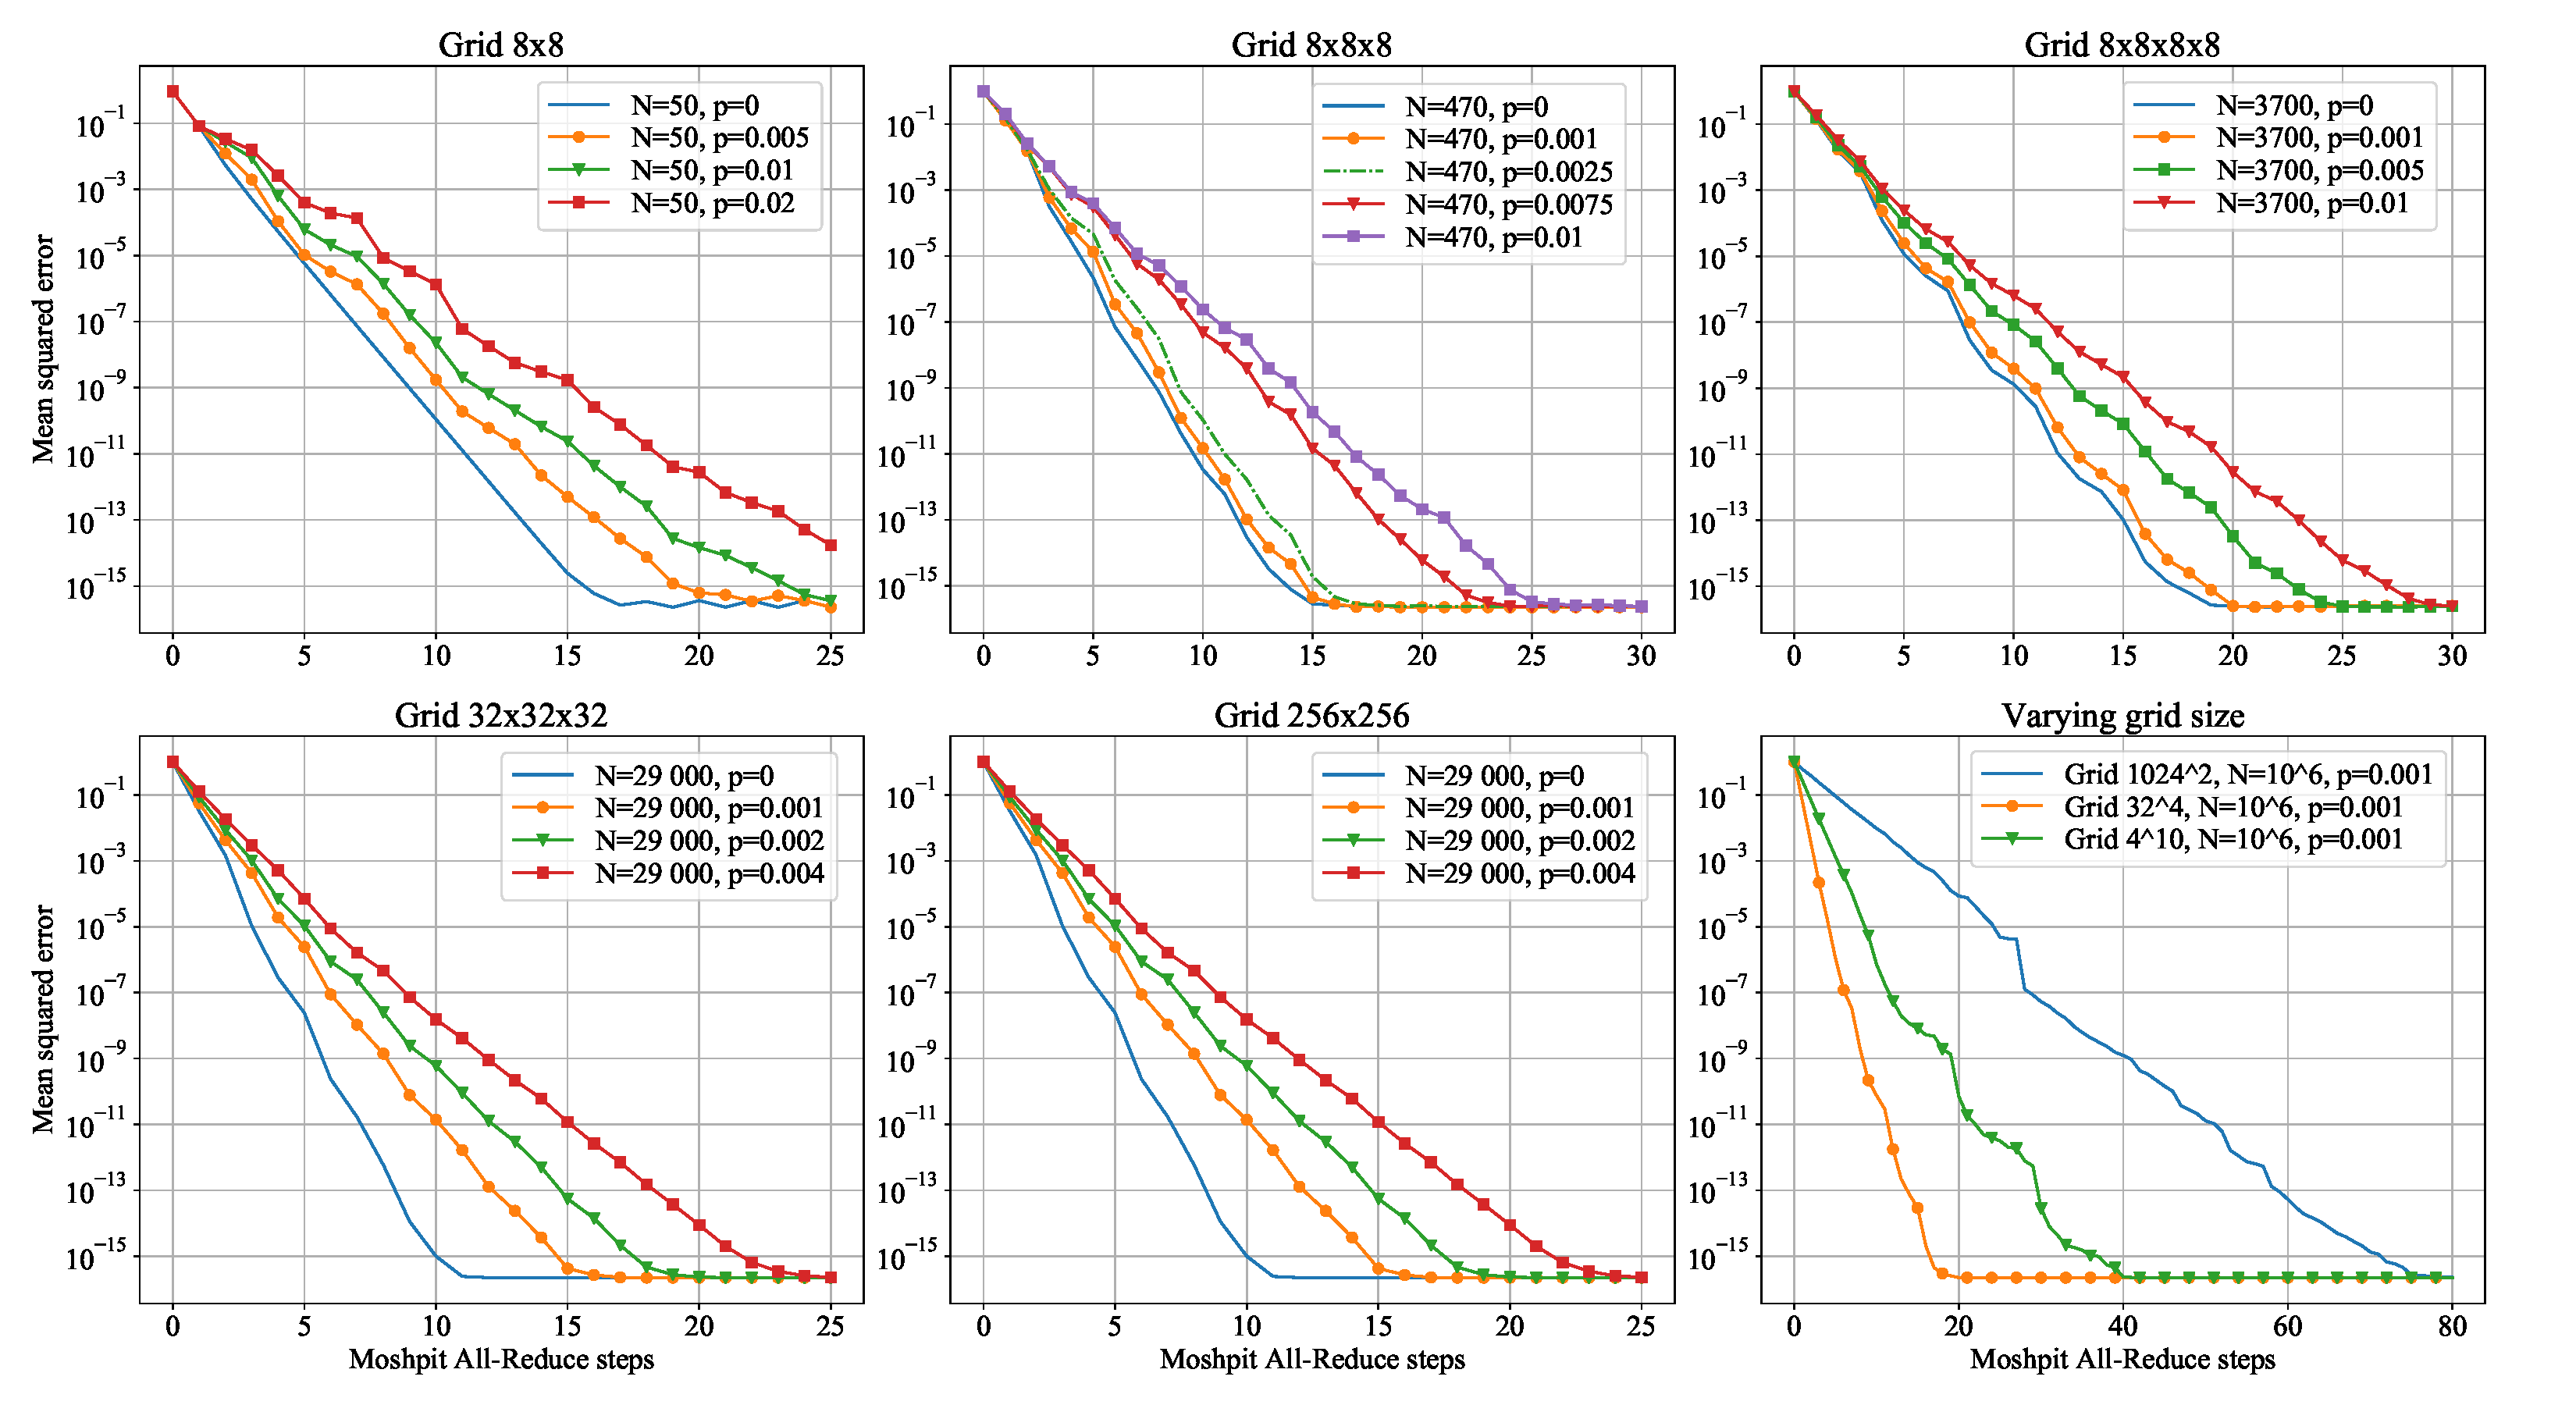
\includegraphics[width=\linewidth]{resources/multiple_graphics.pdf}
    \vspace{-20pt}
    \caption{Averaging error of Moshpit All-Reduce as a function of the iteration number for different configurations and failure rates.}
    \label{fig:many_averagings}
\end{figure}

\section{Additional image classification experiments}
\label{sect:extra_classification}

Aside from the two evaluation scenarios provided in~\ref{sect:experiments_vision}, we also measure the performance of Moshpit-SGD in a non-distributed setup, i.e. on a single server with multiple GPUs. We conduct this experiment on the same $8{\times}$ V100 machine that was used in the \textbf{homogeneous} setup for training ALBERT (see Appendix~\ref{sect:detailed_setup_albert}).

\begin{figure}[h]
    \centering
    \begin{tabular}{cc}
    \hspace{-10pt}
        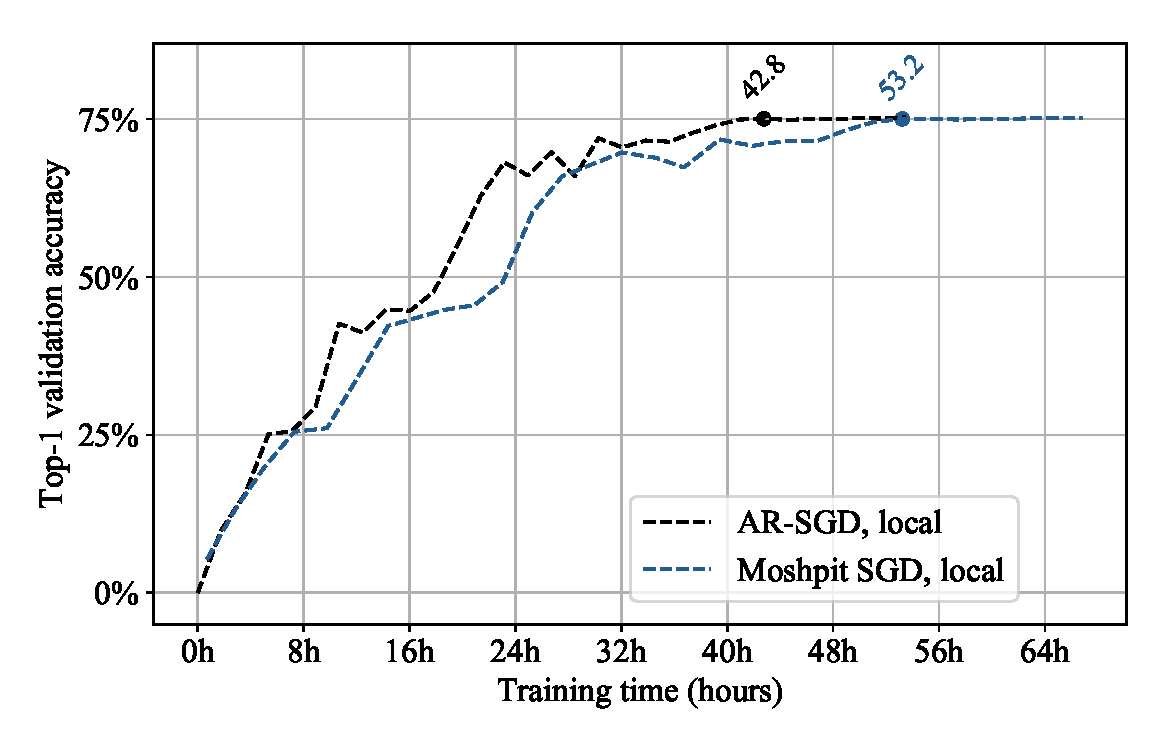
\includegraphics[width=0.5\textwidth]{resources/resnet50_local.pdf} &
        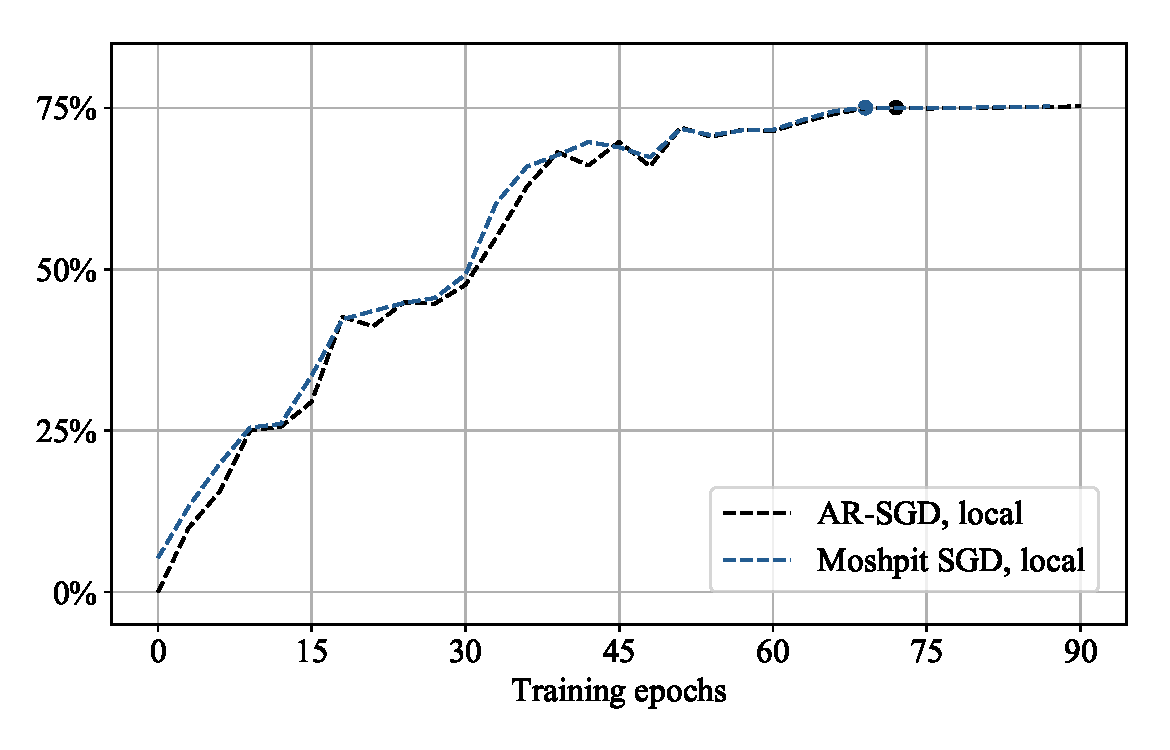
\includegraphics[width=0.5\textwidth]{resources/resnet50_local_epochs.pdf}
    \end{tabular}
    \caption{
    ResNet-50 top-1 validation accuracy on ImageNet when training on a single node with $8{\times}$ V100-PCIe GPUs.
    \textbf{(Left)} Convergence in terms of training time, \textbf{(Right)} Convergence in terms of training epochs}
    \label{fig:resnet_local}\vspace{-8pt}
\end{figure}

As Figure~\ref{fig:resnet_local} demonstrates, Moshpit SGD is slower than AR-SGD by approximately $25\%$. This result is expected, since our implementation of Moshpit All-Reduce is more general and communicates over a TCP connection, whereas AR-SGD uses direct peer-to-peer GPU communication over PCIe. On average, this incurs a slowdown of $27\%$ in terms of training time.

\end{document}